% mnras_template.tex
%
% LaTeX template for creating an MNRAS paper
%
% v3.0 released 14 May 2015
% (version numbers match those of mnras.cls)
%
% Copyright (C) Royal Astronomical Society 2015
% Authors:
% Keith T. Smith (Royal Astronomical Society)

% Change log
%
% v3.0 May 2015
%    Renamed to match the new package name
%    Version number matches mnras.cls
%    A few minor tweaks to wording
% v1.0 September 2013
%    Beta testing only - never publicly released
%    First version: a simple (ish) template for creating an MNRAS paper

%%%%%%%%%%%%%%%%%%%%%%%%%%%%%%%%%%%%%%%%%%%%%%%%%%
% Basic setup. Most papers should leave these options alone.
% \documentclass[a4paper,fleqn,usenatbib]{../mnras}
\documentclass[a4paper,fleqn,usenatbib]{mnras}

% MNRAS is set in Times font. If you don't have this installed (most LaTeX
% installations will be fine) or prefer the old Computer Modern fonts, comment
% out the following line
% \usepackage{newtxtext,newtxmath}
% Depending on your LaTeX fonts installation, you might get better results with one of these:
% \usepackage{mathptmx}
% \usepackage{txfonts}

% Use vector fonts, so it zooms properly in on-screen viewing software
% Don't change these lines unless you know what you are doing
\usepackage[T1]{fontenc}
\usepackage{ae,aecompl}
% \pdfminorversion=5

%%%%% AUTHORS - PLACE YOUR OWN PACKAGES HERE %%%%%

% Only include extra packages if you really need them. Common packages are:
\usepackage{graphicx}	% Including figure files
\usepackage{amsmath}	% Advanced maths commands
\usepackage{amssymb}	% Extra maths symbols
\usepackage[flushleft]{threeparttable} % For table notes
\usepackage[caption=false]{subfig} % For subfloats

%%%%%%%%%%%%%%%%%%%%%%%%%%%%%%%%%%%%%%%%%%%%%%%%%%

%%%%% AUTHORS - PLACE YOUR OWN COMMANDS HERE %%%%%

% Please keep new commands to a minimum, and use \newcommand not \def to avoid
% overwriting existing commands. Example:
%\newcommand{\pcm}{\,cm$^{-2}$}	% per cm-squared
\newcommand{\Nant}{N_\textrm{A}}
\newcommand{\Ngrid}{N_\textrm{g}} 
\newcommand{\Npix}{N_{\text{pix}}}
\newcommand{\dif}{\mathrm{d}}

%%%%%%%%%%%%%%%%%%%%%%%%%%%%%%%%%%%%%%%%%%%%%%%%%%

%%%%%%%%%%%%%%%%%%% TITLE PAGE %%%%%%%%%%%%%%%%%%%

% Title of the paper, and the short title which is used in the headers.
% Keep the title short and informative.
\title[E-field Parallel Imaging Correlator]{A Generic and Efficient E-field Parallel Imaging Correlator for Next-Generation Radio Telescopes}

% The list of authors, and the short list which is used in the headers.
% If you need two or more lines of authors, add an extra line using \newauthor
\author[Thyagarajan et al.]{
Nithyanandan Thyagarajan,$^{1}$\thanks{E-mail: t\_nithyanandan@asu.edu}
Adam P. Beardsley,$^{1}$
Judd D. Bowman$^{1}$
\newauthor
and Miguel F. Morales$^{2}$
\\
% List of institutions
$^{1}$Arizona State University, School of Earth and Space Exploration, Tempe, AZ 85287, USA\\
$^{2}$University of Washington, Department of Physics, Seattle, WA 98195, USA\\
}

% These dates will be filled out by the publisher
\date{Accepted XXX. Received YYY; in original form ZZZ}

% Enter the current year, for the copyright statements etc.
\pubyear{2015}

% Don't change these lines
\begin{document}
\label{firstpage}
\pagerange{\pageref{firstpage}--\pageref{lastpage}}
\maketitle

% Abstract of the paper
\begin{abstract}
Modern radio telescopes are favouring densely packed array layouts with large numbers of antennas ($\Nant\gtrsim 1000$). Since the complexity of traditional correlators scales as $\mathcal{O}(\Nant^2)$, there will be a steep cost for realizing the full imaging potential of these powerful instruments. Through our generic and efficient E-field Parallel Imaging Correlator (EPIC), we present the first software demonstration of a generalized direct imaging algorithm, namely, the Modular Optimal Frequency Fourier (MOFF) imager. It takes advantage of the multiplication-convolution theorem of Fourier transforms. Not only does it bring down the cost for dense layouts to $\mathcal{O}(\Nant\log_2\Nant)$ but can also image from irregular layouts and heterogeneous arrays of antennas. EPIC is highly modular and parallelizable, implemented in object oriented Python, and publicly available. We have verified the images produced to be equivalent to those produced using traditional techniques to within a precision set by gridding coarseness. We have also validated our implementation on data observed with the Long Wavelength Array (LWA). {\bf We have demonstrated its versatility to image with heterogeneous arrays by showing that it robustly estimates the input sky model while wrong assumptions about array homogeneity lead to systematic mis-estimates.} Antenna layouts with dense filling factors consisting of a large number of antennas such as LWA, the Square Kilometre Array, Hydrogen Epoch of Reionization Array, and Canadian Hydrogen Intensity Mapping Experiment will gain significant computational advantage by deploying EPIC. Inherent availability of calibrated time-domain images on digitizer writeout time-scales and vastly lower I/O bandwidth relative to visibility-based systems will make it a prime candidate for transient searches of Fast Radio Bursts (FRB) as well as planetary and exoplanetary phenomena. 
\end{abstract}

% Select between one and six entries from the list of approved keywords.
% Don't make up new ones.
\begin{keywords}
instrumentation: interferometers -- techniques: image processing -- techniques: interferometric
\end{keywords}

%%%%%%%%%%%%%%%%% BODY OF PAPER %%%%%%%%%%%%%%%%%%

\section{Introduction}

Radio astronomy is entering an era in which interferometers of hundreds to thousands of individual antennas are needed to achieve desired survey speeds. Nowhere is this more apparent than at radio frequencies below 1.4 GHz. The study of the history of hydrogen gas throughout the universe's evolution is pushing technology development towards arrays of low-cost antennas with large fields of view and densely packed layouts. Similarly, the search for transient objects and regular monitoring of the time-dependent sky is driving instruments in the same direction with the added requirement of fast read-outs. A number of new telescopes are being or were developed around the world based on this new paradigm, including the Hydrogen Epoch of Reionization Array\footnote{http://reionization.org} (HERA; \citealt{deb16}), the Murchison Widefield Array (MWA; \citealt{tin13,bow13}), the {\bf Donald~C.~Backer} Precision Array for Probing the Epoch of Reionization (PAPER; \citealt{par10}), the LOw Frequency ARray (LOFAR; \citealt{van13}), the Canadian Hydrogen Intensity Mapping Experiment (CHIME; \citealt{ban14}), the Long Wavelength Array (LWA; \citealt{ell13}), and the low frequency Square Kilometer Array (SKA1-Low; \citealt{mel13}).

This paradigm shift requires a fundamentally new approach to the design of
digital correlators \citep{lon00}. Modern correlators calculate the cross-power
correlation between all antenna pairs in many narrow frequencies, forming
\emph{visibilities}, the fundamental measurement of traditional radio
interferometers. The computational requirements for a modern FX correlator scale
with the number of antenna pairs, or the square of the number of antennas $\sim
\Nant^2$ \citep{bun04}. For this reason traditional correlators have difficulty
scaling to thousands of antennas. As an example, the full HERA correlator for
352 dishes with 200 MHz of bandwidth requires 212 trillion complex multiplies
and adds per second (TMACS). Future arrays with thousands of collecting elements
will require orders of magnitude more computation, making the correlator the
dominant cost.

For certain classes of radio arrays there is an alternative to the FX correlator
that can lower the computational burden by directly performing a spatial Fast
Fourier Transform \citep[FFT;][]{coo65} on the electric fields measured by each 
antenna in the array at each time step, removing the cross-correlation step. 
This relieves the computational scaling from the harsh $\Nant^2$ to the more 
gentle envelope of $\sim\Ngrid\log_2\Ngrid$, where $\Ngrid$ is the number of 
grid points in the Fourier transform \citep[e.g.][]{mor11,teg09,teg10}. This 
architecture is often referred to as a ``direct imaging'' correlator because it 
eliminates the intermediate cross-correlation data products of the FX and XF 
correlators, but instead directly forms images from the electric field 
measurements.

Direct imaging correlators have begun to be explored on deployed arrays including
the Basic Element for SKA Training II (BEST-2) array \citep{fos14}, the Omniscope
\citep{zhe14}, and an earlier incarnation at higher frequencies with the intent
of pulsar timing \citep{oto94, dai00}. However, each of these examples make
assumptions about the redundancy of the array layout, and require the collecting
elements are identical. On the other hand, the MOFF algorithm achieves the same
$\Ngrid \log_2 \Ngrid$ computational scaling without placing any restriction on
antenna placement, can accommodate non-identical antennas, and is provably 
optimal \citep{mor11}. This algorithm uses the antenna beam patterns to 
grid the electric field measurements to a regular grid in the software 
holography/A-transpose fashion \citep{mor09,bha08,teg97b} before performing the
spatial FFT. This process has been shown to theoretically produce a data product
identical to images produced from traditional visibility-based techniques.

Here we present the first software implementation of the MOFF correlator, and
announce the public release of the E-field Parallel Imaging Correlator (EPIC)
code. EPIC is a highly parallel, object oriented Python package that primarily 
implements the MOFF imaging algorithm besides emulating real-life telescopes and 
FX/XF correlators in software, and includes a visibility-based imaging technique 
for reference. It is intended to provide a development platform to test different 
imaging approaches, characterize scaling relations and serve as a stepping stone 
for real-life GPU/FPGA-based implementation on telescopes.

We begin with a technical description of the algorithm in \S\ref{sec:math}, then discuss our particular implementation in \S\ref{sec:software}. We then verify the output data quality from our code in \S\ref{sec:verify} by presenting simulated images from both the EPIC correlator and comparing to a simulated FX correlator. We also demonstrate the performance with real-world data from the LWA. {\bf \S\ref{sec:versatility} demonstrates its ability to robustly image data from heterogeneous arrays.} In \S\ref{sec:analysis}, we explore the scalability of the algorithm in the context of several array design choices. We identify specific array design classes where the EPIC correlator -- is computationally more efficient; and in the field of transients, demands significantly lesser I/O bandwidth relative to visibility-based approaches. We conclude and discuss future research prospects in \S\ref{sec:conclusions}.

\section{Mathematical Framework}\label{sec:math}

We provide a brief summary of the mathematical equivalence of the MOFF and 
FX correlators detailed in \citet{mor11}. We first relate the image produced 
from visibilities to the electric fields of astrophysical sources, then show that 
operations can be reordered to produce the same images at a lower 
computational cost.

Electric fields from astrophysical sources, $\mathcal{E}(\hat{\mathbf{s}}, f, t)$, in the sky coordinate system denoted by the unit vector $\hat{\mathbf{s}}$, propagate towards the observer as:
\begin{align}
  E(\mathbf{r}, f, t) &= \int \mathcal{E}(\hat{\mathbf{s}},f,t)\,e^{-2\pi i f\mathbf{r}\cdot\hat{\mathbf{s}}/c}\,\dif\Omega,
\end{align}
where, $\mathbf{r}$ denotes the observer's location, {\bf $f$ is the frequency of radiation, $c$ is the speed of light, $t$ denotes time} and $E(\mathbf{r}, f, t)$ is the propagated electric field. Thus the propagated electric field is a linear superposition of the electric fields emanating from astronomical sources with appropriate complex phases. {\bf Ignoring wide-field effects}, it can be {\bf simplified as} a Fourier transform of the electric fields in the sky coordinates. 

An antenna, {\bf located at $\mathbf{r}_a$ (indexed by $a$)}, measures a phased sum of these propagated electric fields over its effective collecting area with an additive receiver noise:
\begin{align}\label{eqn:measured-E-field}
  E_a(f,t) &= \int W_a(\mathbf{r}-\mathbf{r}_a,f,t)\,E(\mathbf{r},f,t)\,\dif^2\mathbf{r} + n_a(f,t) \\
           &= \int W_a(\mathbf{r}-\mathbf{r}_a,f,t) \nonumber \\
           &\quad \times \left[ \int \mathcal{E}(\hat{\mathbf{s}},f,t)\,e^{-2\pi i f\mathbf{r}\cdot\hat{\mathbf{s}}/c}\,\dif\Omega \right] \dif^2\mathbf{r} + n_a(f,t) \\
           &= \int \mathcal{W}_a(\hat{\mathbf{s}},f,t)\,\mathcal{E}(\hat{\mathbf{s}},f,t)\,e^{-2\pi i f\mathbf{r}_a\!\cdot\,\hat{\mathbf{s}}/c}\,\dif\Omega + n_a(f,t)
\end{align}
where, {\bf $W_a(\mathbf{r},f,t)$ is the aperture electric field illumination pattern of the antenna and its Fourier transform, $\mathcal{W}_a(\hat{\mathbf{s}},f,t)$, is the directional antenna voltage response at a given frequency and time}.

Interferometers measure {\it visibilities} -- the degree of coherence between electric fields measured by a pair of antennas \citep{van34,zer38,tho01}. A visibility, $V_{ab}$, can be written as:
\begin{align}
  V_{ab}(f,t) &= \left\langle E_a(f,t)E_b^\star(f,t) \right\rangle_t \label{eqn:cc-vis}\hfill\\
              &= \left\langle \left[ \int \mathcal{W}_a(\hat{\mathbf{s}},f,t)\,\mathcal{E}(\hat{\mathbf{s}},f,t)\,e^{-2\pi i f\mathbf{r}_a\!\cdot\,\hat{\mathbf{s}}/c}\,\dif\Omega\right.\right. \nonumber\\
              &\qquad\qquad\qquad\qquad\qquad\qquad\qquad\quad + \left. n_a(f,t) \vphantom{\int}\right] \nonumber\\
              &\quad \times \left[ \int \mathcal{W}^\star_b(\hat{\mathbf{s'}},f,t)\,\mathcal{E}^\star (\hat{\mathbf{s'}},f,t)\,e^{2\pi i f\mathbf{r}_b\!\cdot\,\hat{\mathbf{s'}}/c}\,\dif\Omega^\prime \right. \nonumber\\
              &\qquad\qquad\qquad\qquad\qquad\qquad\qquad\quad + \left.\left. n^\star_b(f,t) \vphantom{\int}\right] \right\rangle_t \nonumber\\
              &= \iint \mathcal{W}_a(\hat{\mathbf{s}},f,t) \mathcal{W}^\star_b(\hat{\mathbf{s'}},f,t) \left\langle \mathcal{E}(\hat{\mathbf{s}},f,t) \mathcal{E}^\star(\hat{\mathbf{s'}},f,t) \right\rangle_t \nonumber\\
              &\qquad\qquad\qquad\qquad \times e^{-2\pi i f(\mathbf{r}_a\!\cdot\,\hat{\mathbf{s}}-\mathbf{r}_b\!\cdot\,\hat{\mathbf{s'}})/c}\,\dif\Omega\,\dif\Omega^\prime \nonumber\\
              &\qquad +\textrm{noise-like cross-terms.}
\end{align}
where we have brought the time average into the integral under the assumption that the aperture illumination pattern does not change over the time-scale of the averaging and $\star$ denotes complex conjugation. {\bf The noise-like cross-terms ideally have zero mean. This expression can be further simplified using the sky brightness}, $\mathcal{I}(\hat{\mathbf{s}},f,t)$, as $\left\langle \mathcal{E}(\hat{\mathbf{s}},f,t)\,\mathcal{E}^\star(\hat{\mathbf{s'}},f,t) \right\rangle_t = \mathcal{I}(\hat{\mathbf{s}},f,t)\,\delta(\hat{\mathbf{s}}-\hat{\mathbf{s'}})$, and defining the antenna-pair sky power response function (or the directional antenna-pair power pattern), $\mathcal{B}_{ab}(\hat{\mathbf{s}})~\equiv~\mathcal{W}_a(\hat{\mathbf{s}},f,t)~\mathcal{W}^\star_b(\hat{\mathbf{s}},f,t)$. The result is the visibility expressed in terms of the sky brightness, the power pattern, and uncorrelated noise terms which we group into $n_{ab}(f,t)$.
\begin{align}\label{eqn:measurement-eqn-1}
  V_{ab}(f,t) &= \int \mathcal{B}_{ab}(\hat{\mathbf{s}},f,t)\,\mathcal{I}(\hat{\mathbf{s}},f,t)\,e^{-2\pi i f\mathbf{r}_{ab}\!\cdot\,\hat{\mathbf{s}}/c}\,\dif\Omega \nonumber\\
  &\qquad\qquad + n_{ab}(f,t),
\end{align}
where, the baseline coordinate $\mathbf{r}_{ab}\equiv\mathbf{r}_a-\mathbf{r}_b$ is the vector separation between the two antennas. This signifies that the visibility ($V_{ab}$) measured between a pair of antennas is obtained by multiplying the sky brightness $\mathcal{I}(\hat{\mathbf{s}},f,t)$ by the antenna power response $\mathcal{B}_{ab}(\hat{\mathbf{s}},f,t)$ and Fourier transforming from the directional coordinates ($\hat{\mathbf{s}}$) to {\bf the measurement plane}, which are then sampled at the locations of the antenna spacings (or baselines), namely, $\mathbf{r}_{ab}$, and added to the noise $n_{ab}$. 

This can be equivalently re-written as:
\begin{align}\label{eqn:software-holography}
  V_{ab}(f,t) &= \int B_{ab}(\mathbf{r}_{ab}-\mathbf{r},f,t) \nonumber\\ 
              &\qquad \times \left[\int I(\hat{\mathbf{s}},f,t)\,e^{-2\pi i f\mathbf{r}.\hat{\mathbf{s}}/c}\,\dif\Omega\right]\dif^2\mathbf{r}\,+\, n_{ab}(f,t),
\end{align}
where, $B_{ab}(\mathbf{r},f,t)$ denotes the {\bf power response of the antenna pair obtained in the measurement plane} by a spatial Fourier transform of $\mathcal{B}_{ab}(\hat{\mathbf{s}},f,t)$. Effectively, the multiplication in image space by $\mathcal{B}_{ab}(\hat{\mathbf{s}},f,t)$ has been replaced by a convolution with $B_{ab}(\mathbf{r},f,t)$ in {\bf measurement plane}. This is the software holographic equivalent of a traditional FX correlator output. {\bf For context, the term ``holography'' is derived from holographic measurements of the complex antenna aperture illumination pattern \citep{ben76,sco77}. In the present context, ``software holography'' refers to the application of this antenna aperture illumination pattern in software for imaging.}

Hereafter, we adopt the matrix notation of \citet{mor11}, where vectors are represented with single coordinates, and matrices are represented by two coordinates denoting the spaces the operator transforms between. Since each frequency is processed independently, we drop the dependence on $f$. In this notation, the above measurement equation can be expressed as:
\begin{align}
  \mathbf{m}(\mathbf{v}) &= \mathbf{B}(\mathbf{v},\mathbf{u})\,\mathbf{F}(\mathbf{u},\hat{\mathbf{s}})\,\boldsymbol{\mathcal{I}}(\hat{\mathbf{s}}) + \mathbf{n}(\mathbf{v}),
\end{align}
where the sky brightness $\boldsymbol{\mathcal{I}}(\hat{\mathbf{s}})$ is Fourier transformed using $\mathbf{F}(\mathbf{u},\hat{\mathbf{s}})$ and the resultant spatial coherence function is weighted and summed using the antenna power response, $\mathbf{B}(\mathbf{v},\mathbf{u})$ in $uv$-space sampled at the baseline location to obtain the measured visibilities:
\begin{align}
  \mathbf{m}(\mathbf{v}) &= \left\langle \mathbf{E}(\mathbf{a})\,\mathbf{E}^\star(\mathbf{a}^\prime)\right\rangle_t, \label{eqn:matrix-cc-vis}
\end{align}
where $\mathbf{m}(\mathbf{v})$ denotes visibilities measured by cross-correlating measured antenna electric fields over all possible pairs of $\mathbf{a}$ and $\mathbf{a}^\prime$. It is the same as equation~\ref{eqn:cc-vis} written in matrix notation.

Using the optimal map-making formalism \citep{teg97a,teg97b}, a software holography image is formed using \citep{mor09}:
\begin{align}
  \boldsymbol{\mathcal{I}}^\prime(\hat{\mathbf{s}}) &= \mathbf{F}^\textrm{T}(\hat{\mathbf{s}},\mathbf{u})\,\mathbf{B}^{\,\textrm{T}}(\mathbf{u},\mathbf{v})\,\mathbf{N}^{-1}(\mathbf{v},\mathbf{v})\,\mathbf{m}(\mathbf{v}) \label{eqn:dirty-image-FX}
\end{align}
where the measured visibilities are weighted by the inverse of the system noise, followed by a gridding process using the holographic antenna power response as the gridding kernel, followed by a Fourier transform to create an image $\boldsymbol{\mathcal{I}}^\prime(\hat{\mathbf{s}})$. This is the {\bf optimally weighted} estimate of the true image $\boldsymbol{\mathcal{I}}(\hat{\mathbf{s}})$ given the visibility measurements.

The intermediate step of gridding with the antenna power response can be expressed as a convolution of a data vector generated by gridding the electric fields directly with the antenna illumination pattern.
\begin{align}
\mathbf{B}^{\,\textrm{T}}(\mathbf{u},\mathbf{v})\,\mathbf{N}^{-1}(\mathbf{v} ,\mathbf{v})\,\mathbf{m}(\mathbf{v}) &= \left\langle \left[\mathbf{W}_a(\mathbf{r},\mathbf{a})\,\widetilde{\mathbf{N}}^\textrm{T}\!(\mathbf{a},\mathbf{a})\, \mathbf{E}^\star(\mathbf{a})\right]\right. \nonumber\\ 
&\,\quad\ast\left.\left[\mathbf{W}^\textrm{T}_a(\mathbf{r},\mathbf{a})\,\widetilde{\mathbf{N}}\!(\mathbf{a},\mathbf{a})\,\mathbf{E}(\mathbf{a})\right]\right\rangle_t, \label{eqn:e-field-conv}
\end{align}
where, $\mathbf{N}^{-1}$ has been expressed as $\widetilde{\mathbf{N}}^\textrm{T}\widetilde{\mathbf{N}}$.

We can then use the multiplication-convolution theorem to move the convolution in Equation~\ref{eqn:e-field-conv} to a square after the Fourier transform in equation~\ref{eqn:dirty-image-FX}.
\begin{align}
  \boldsymbol{\mathcal{I}}^\prime(\hat{\mathbf{s}}) &= \left\langle \left|\,\mathbf{F}^\textrm{T}(\hat{\mathbf{s}},\mathbf{r})\,\mathbf{W}^\textrm{T}(\mathbf{r},\mathbf{a})\,\widetilde{\mathbf{N}}(\mathbf{a},\mathbf{a})\,\mathbf{E}(\mathbf{a})\,\right|^2\right\rangle_t. \label{eqn:dirty-image-MOFF}
\end{align}
The term inside the angular brackets before squaring has a very similar form as that in equation~\ref{eqn:dirty-image-FX}. It signifies that the measured antenna electric fields are weighted by the antenna noise, weighted and gridded by the antenna aperture kernel, Fourier transformed and finally squared to obtain the same image estimate that would have been obtained using equation~\ref{eqn:dirty-image-FX}. 

Equation~\ref{eqn:dirty-image-MOFF} is the optimal imaging equation used by the MOFF algorithm. While mathematically equivalent to equation~\ref{eqn:dirty-image-FX}, squaring in image space rather than convolving in $uv$ space potentially saves orders of magnitude in computation.

There are some important differences between the two techniques:
\begin{enumerate}
\item The time-averaging cannot be performed on a stochastic measurement but only on its statistical properties. In visibility-based imaging, the visibilities measured between antenna pairs represent spatial correlations which can be time-averaged followed by gridding and imaging. However, in MOFF imaging both antenna and gridded electric fields are stochastic and therefore must be imaged and squared before time-averaging. 
\item In visibility-based imaging, electric fields measured by antennas are not correlated with themselves and hence lack zero spacing measurements. In contrast, in MOFF imaging, since the gridded electric fields are imaged and squared, they retain information from auto-correlated electric fields at zero spacing {\bf but can be removed in EPIC.}
\end{enumerate} 

\section{Software Implementation}\label{sec:software}

We have implemented the MOFF imaging technique in our ``E-field Parallel Imaging Correlator'' -- a highly parallelized Object Oriented Python package,\footnote{The E-field Parallel Imaging Correlator (EPIC) package can be accessed at https://github.com/nithyanandan/EPIC} now publicly available. Besides implementing the MOFF imaging algorithm it also includes {\bf a simulator for generating electric fields from a sky model and a visibility-based imaging using the software holography technique.}

EPIC can accept dual-polarization inputs and produce images of all four instrumental cross-polarizations. Currently two data input formats exist for reading in the electric field time samples measured by the antennas -- simulated electric fields based on a sky model using the simulator packaged with EPIC; and LWA data. Efforts to build interfaces for data from other telescopes are underway.

Fig.~\ref{fig:MOFF-flowchart} shows the flowchart for MOFF imaging. The propagated electric fields are shown on the left at different time stamps, $t_1\ldots t_\textrm{M}$. At each time stamp, the electric fields measured by antennas are denoted by $\widetilde{E}_1(t)\ldots \widetilde{E}_\textrm{N}(t)$. The F-engine performs a temporal Fourier transform on the electric field time-series to obtain electric field spectra $E_1(f)\ldots E_\textrm{N}(f)$ ($\mathbf{E}(\mathbf{a})$ in matrix notation) for each of the antennas. Each of the complex antenna gains are calibrated to correct the corresponding electric field spectra. These calibrated electric fields are gridded using an antenna-based gridding convolution function after which it is spatially Fourier transformed and squared to obtain an image cube for every time stamp. These images are then time-averaged to obtain the accumulated image $\mathcal{I}^\prime(f)$ ($\boldsymbol{\mathcal{I}^\prime}(\hat{\mathbf{s}})$ in matrix notation).

\begin{figure}
  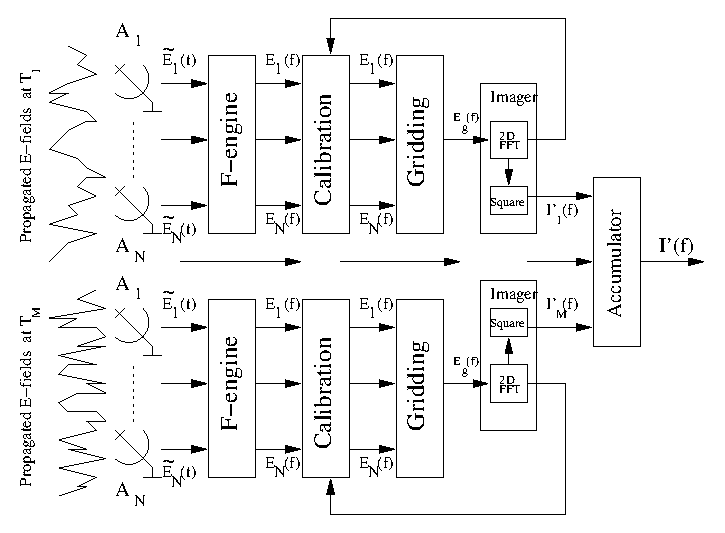
\includegraphics[width=\columnwidth]{figure1}
  % 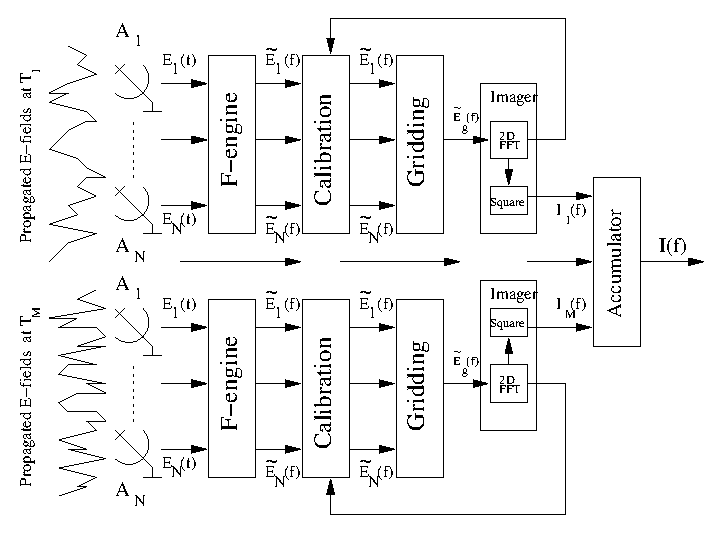
\includegraphics[width=\columnwidth]{MOFF_flowchart}
  % 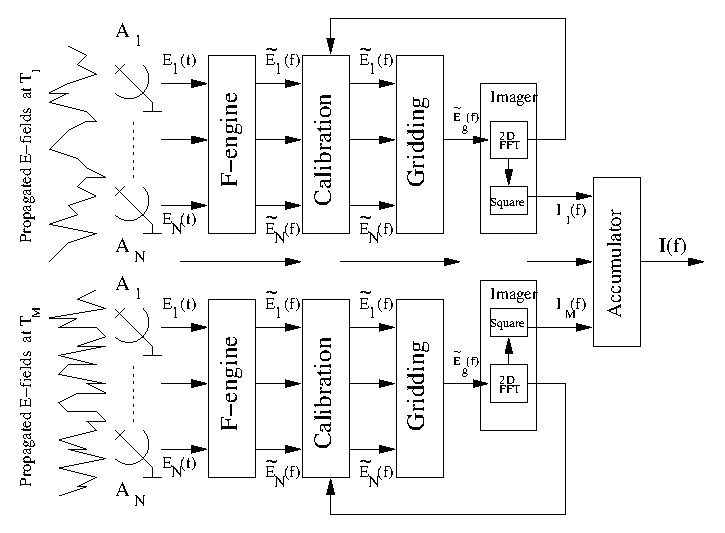
\includegraphics[width=\columnwidth]{MOFF_flowchart.eps}
  \caption{A flowchart of MOFF imaging in EPIC. The propagated electric fields shown on the left are measured as time-series $\widetilde{E}_1(t)\ldots \widetilde{E}_\textrm{N}(t)$ by the antennas $\textrm{A}_1\ldots \textrm{A}_\textrm{N}$ which are then Fourier transformed by the F-engine to produce electric field spectra $E_1(f)\ldots E_\textrm{N}(f)$. They are calibrated and gridded. The gridded electric fields $E_\textrm{g}(f)$ from each time series are imaged to produce images $\mathcal{I}^\prime_1(f)\ldots \mathcal{I}^\prime_\textrm{M}(f)$. These images are time-averaged to obtain the final image $\mathcal{I}^\prime(f)$.}
  \label{fig:MOFF-flowchart}
\end{figure}

Fig.~\ref{fig:FX-flowchart} shows the flowchart for a visibility-based software holographic imaging from a FX correlator. The antenna-based F-engine is identical to that in the MOFF processing. The electric field spectra from each antenna are then cross-multiplied in the X-engine with those from all other antennas to obtain the visibilities $V_\textrm{ab}(f,t)$ ($\mathbf{m}(\mathbf{v})$ in matrix notation). They are calibrated and time-averaged to obtain $\langle V_\textrm{ab}(f)\rangle$ which are then gridded and imaged to obtain the image $\mathcal{I}^\prime(f)$. The $\mathcal{I}^\prime(f)$ obtained from both techniques are theoretically identical as explained in \S\ref{sec:math}.

\begin{figure}
  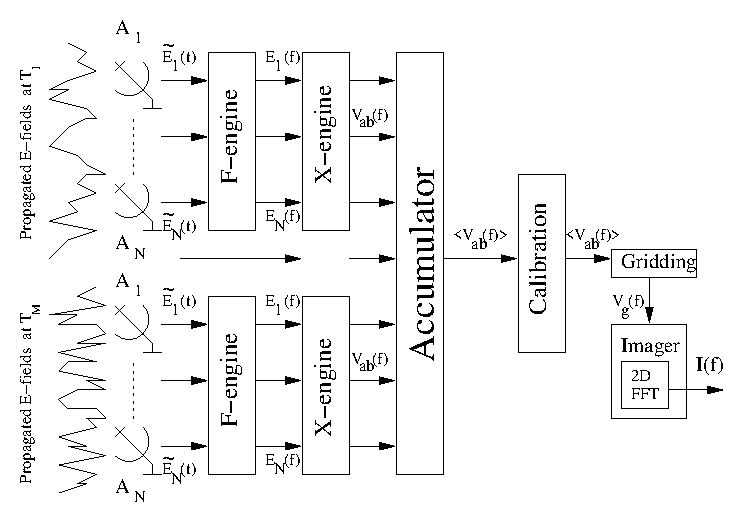
\includegraphics[width=\columnwidth]{figure2}
  % 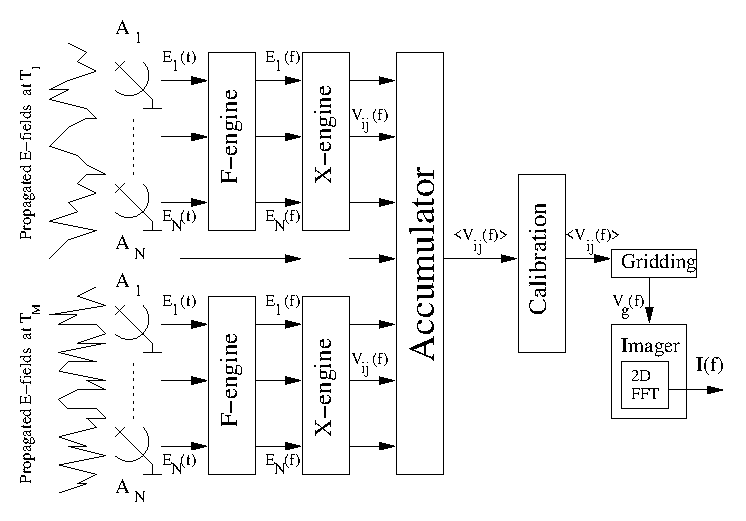
\includegraphics[width=\columnwidth]{FX_flowchart}
  % 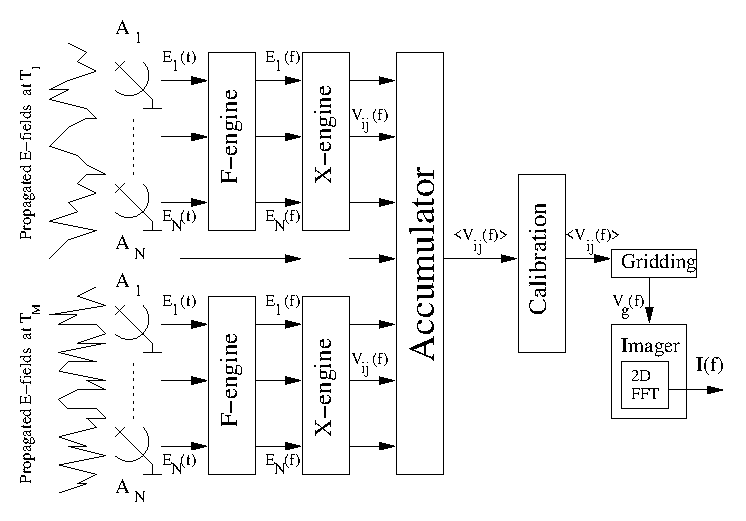
\includegraphics[width=\columnwidth]{FX_flowchart.eps}
  \caption{A flowchart of visibility-based software holographic imaging in EPIC. The FX process flow shares the F-engine with the MOFF process. Following the F-engine, the electric fields pass through the X-engine to produce visibilities $V_\textrm{ab}(f,t)$ which are calibrated and time-averaged. Then they are gridded to obtain the gridded visibilities $V_\textrm{g}(f)$ which are then Fourier transformed to obtain the image, $\mathcal{I}^\prime(f)$.}
  \label{fig:FX-flowchart}
\end{figure}

Here we discuss the components of these architectures in detail. 

\par\medskip
\noindent {\bf Antenna-to-Grid Mapping}
\par\medskip
\noindent A grid is generated on the coordinate system in which antenna 
locations are specified with a grid spacing. The grid spacing can be controlled 
by the user. By default, it is set to be $\le\lambda/2$ even at the 
lowest wavelength to ensure there is no aliasing even from regions of the sky 
far away from the field of view. The number of locations on the grid is 
restricted to be a power of 2 for efficient use of FFT. 

The gridding kernel in the simplest case is given by the antenna aperture
illumination function, $W(\mathbf{r}-\mathbf{r}_a)$, which can
be specified either by a functional form or as a table of values against 
locations around the antennas. A nearest neighbor mapping from all antenna 
footprints to grid locations is created using an efficient k-d tree algorithm 
\citep{man99}. There is no restriction here that the aperture illumination 
function has to be identical across antennas. 

In the most general case, this gridding kernel could contain information on
$w$-projection effects, and other time-dependent ionospheric effects. For a
stationary antenna array in the absence of any time-dependent effects, this
mapping must only be determined once in the antenna array coordinate frame. The
antenna-to-grid mapping matrix, $\mathbf{M}(\mathbf{r},\mathbf{a})$ is described
as a transformation matrix from the space of measured electric fields by the 
antennas ($\mathbf{a}$) to the antenna array grid denoted by the coordinate 
$\mathbf{r}$. Since each antenna occupies a footprint typically the size of its 
aperture, $\mathbf{M}(\mathbf{r},\mathbf{a})$, which is generally of size
$\Ngrid\times \Nant$, reduces to a sparse block-diagonal matrix
with only $\Nant$ blocks and roughly $N_\textrm{k}$ non-zero entries per
block, where $N_\textrm{k}$ is the number of grid points that fall inside an
antenna's footprint. This sparse matrix is stored in a Compressed Sparse Row 
(CSR) format. Fig.~\ref{fig:a2g-mapping} illustrates the antenna-to-grid mapping
matrix and the grid containing the mapped aperture footprints of the antennas.

\begin{figure}
  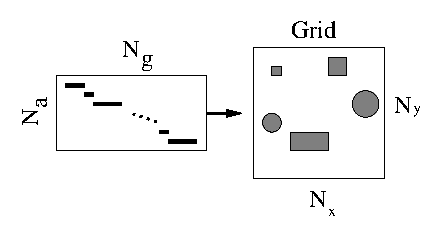
\includegraphics[width=\columnwidth]{figure3}
  % 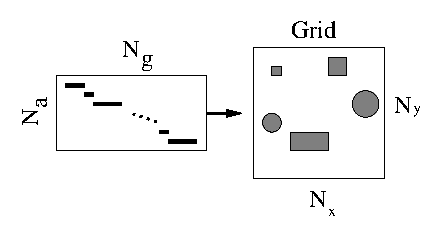
\includegraphics[width=\columnwidth]{a2g_mapping}
  % 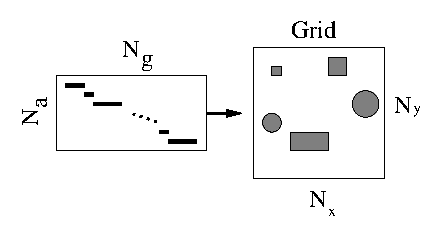
\includegraphics[width=\columnwidth]{a2g_mapping.eps}
  \caption{Block diagram of an antenna-to-grid mapping. A sparse block-diagonal
    matrix of total size $\Ngrid\times \Nant$ is created where each
    block contains roughly the number of pixels covered by the respective kernel.
    The antenna aperture illumination kernels do not have to be identical to each
    other. A discrete set of arbitrarily placed antennas are now placed on to a
    regular grid.}
  \label{fig:a2g-mapping}
\end{figure}

\par\medskip
\noindent {\bf Temporal Fourier transform}
\par\medskip
\noindent This module is common to the MOFF and visibility-based imaging 
techniques. Time samples of electric fields measured by the antenna and 
digitized by the A/D converter is Fourier transformed to generate electric 
field spectra. This step can be parallelized across antennas%  as shown in 
% Fig.~\ref{fig:f-engine}
. The output is then fed to either MOFF or 
visibility-based imaging pipelines.

% \begin{figure}
%   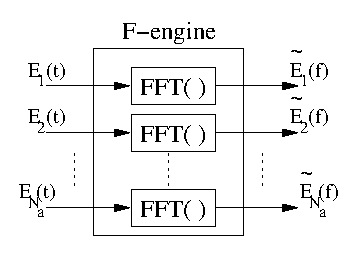
\includegraphics[width=\columnwidth]{figure4}
%   % \includegraphics[width=\columnwidth]{parallel_F_engine}
%   % \includegraphics[width=\columnwidth]{parallel_F_engine.eps}
%   \caption{Block diagram of a F-engine. The electric field data streams from
%     antennas are Fourier transformed in parallel to generate electric field
%     spectra.}
%   \label{fig:f-engine}
% \end{figure}

\par\medskip
\noindent {\bf Calibration}
\par\medskip
\noindent Calibration of direct imaging correlators remains a challenge. Contrary
to the FX data flow, direct imagers mix the signals from all antennas before
averaging and writing to disk. It is therefore essential to apply gain solutions 
before the gridding step. Previous efforts have resorted to applying FX-generated
calibration solutions \citep{zhe14,fos14}, or integrating a dedicated FX 
correlator which periodically forms the full visibility matrix 
\citep{wij09,dev09}. 

In a companion paper \citep{bea16}, we demonstrate a novel calibration 
technique (EPICal) which leverages the data products formed by direct imaging 
correlators to estimate antenna complex gains. This method correlates the antenna 
electric field signals with an image pixel from the output of the correlator in 
the feedback calibration fashion outlined in \citealt{mor11} (illustrated in 
Fig.~\ref{fig:MOFF-flowchart} by the arrow leading from the imager to the 
calibration block). Furthermore it allows for arbitrarily complex sky models, 
and following the MOFF algorithm places no restriction on array layout, and 
accounts for non-identical antenna beam patterns. Direction dependent calibration 
can be achieved by correlating antenna signals with output pixels in the 
direction of $N_\textrm{c}$ calibration sources, then fitting for a functional 
model of the sky. Since antennas are only correlated with calibrator pixels, the 
computational complexity scales as $\sim N_\textrm{a} N_\textrm{c}$. {\bf The calibration performance of EPIC is explored for varying levels of completeness of sky model in \citet{bea16}.}

The calibration module included in EPIC allows for application of pre-determined 
calibration solutions, or can solve for the complex gains using the EPICal 
algorithm.

\par\medskip
\noindent {\bf Gridding Convolution}
\par\medskip
\noindent The antenna array aperture illumination over the entire grid, $W(\mathbf{r})$, is obtained by a projection of the individual antenna aperture illuminations:
\begin{align}\label{eqn:gridding-convolution}
  W(\mathbf{r}) &= \sum_a W_a(\mathbf{r}-\mathbf{r}_a),
\end{align}
or in matrix notation,
\begin{align}
  \mathbf{W}(\mathbf{r}) &= \mathbf{M}(\mathbf{r},\mathbf{a})\,\mathbf{I}(\mathbf{a}),
\end{align}
where, $\mathbf{I}(\mathbf{a})$ is a row of ones denoting coverage of the grid by kernel footprints of antennas. This is achieved by efficient multiplication with the sparse matrix created in the antenna-to-grid mapping process using the sparse matrices module in Python SciPy package. Unless $\mathbf{W}(\mathbf{r})$ includes time-dependent effects of the ionosphere or the instrument, it needs to be computed just once for the entire observation. However, the gridding of electric fields must be computed at every readout of the electric field spectra,
\begin{align}
  \mathbf{E}(\mathbf{r}) &= \mathbf{M}(\mathbf{r},\mathbf{a})\,\mathbf{E}(\mathbf{a}).
\end{align}

\par\medskip
\noindent {\bf Spatial Fourier Transform}
\par\medskip
\noindent Before the spatial Fourier transform, the gridded electric fields are 
padded with zeros in order to match the grid size and angular size of each image 
pixel that would have been obtained with the software holography output from an 
FX correlator. 

In MOFF imaging, these are spatially Fourier transformed followed by a squaring
operation at every time stamp for every frequency channel. In visibility-based 
imaging, the spatial Fourier transform is performed only once per integration 
time-scale and does not include a squaring operation.

\par\medskip
\noindent {\bf Time-averaging}
\par\medskip
\noindent In MOFF imaging, the measured antenna electric fields and the 
corresponding holographic electric field images are zero-mean stochastic 
quantities. Hence, they cannot be time-averaged to reduce noise. The statistical 
quantity stable with time in this case are the square of the holographic 
electric field images. Thus, squared images have to be formed at every instant 
of time before averaging as indicated in equation~\ref{eqn:dirty-image-MOFF}.

In contrast, visibilities measured by an antenna are statistically stable within
an integration time interval. Hence, they are averaged after calibration as shown
in equation~\ref{eqn:cc-vis}. It is advantageous to average them in visibilities
before imaging because the repeated cost of spatial FFT can be avoided. Since 
this averaging has been performed already on the visibilities over an integration 
time-scale, the imaging step has to be performed only once per integration cycle. 

A high level software architecture of the EPIC package is described in the 
appendix \S\ref{sec:software-modules} for the interested reader.

\section{Verification}\label{sec:verify}

In order to verify the accuracy of the EPIC code, we characterize the images 
produced through simulations. We simulate electric field streams from a model 
sky and process the data through both the MOFF and a visibility-based imaging 
algorithm. We then compare the output images to demonstrate their equivalence.

\subsection{Simulations}\label{sec:sim}

We use the EPIC simulator to generate stochastic electric field samples from a sky model consisting of 10 point sources of random flux densities $>10$~Jy each at random locations. In our simulations, we use 64 frequency channels each of width $\Delta f = 40$~kHz. The number of time stamps integrated in one integration cycle was kept at eight where each A/D timeseries is $1/\Delta f=25\,\mu$s long. We use the MWA array layout \citep{bea12} for demonstration. Only the inner 51 tiles within a square bounding box of 150~m on each side were used. We assumed all tiles are identical and have a square shaped electric field illumination footprint 4.4~m on each side. Besides the stochastic sky noise present in the simulated electric fields, no noise from the instrument is added.

\subsection{Antenna auto-correlations}\label{sec:rm-autocorr}

Before the outputs can be compared, we describe the elimination of a distinct difference between the two techniques. The squaring operation under MOFF imaging in the image plane introduces antenna auto-correlations around the zero spacing in the $uv$-plane which are absent in traditional visibility-based imaging. In order to facilitate a robust comparison between MOFF and visibility-based imaging techniques, these auto-correlations are removed from the MOFF algorithm output, which is otherwise not an essential part of the core algorithm. We describe below how they are removed. 

The shape and extent of these auto-correlations can be estimated from the 
antenna aperture illumination pattern. The aperture illumination patterns
are already available from the gridding step. Fig.~\ref{fig:autocorr_wts_PB} 
shows the estimated weights from antenna auto-correlations in the $uv$-plane 
(left) and the corresponding response in the image plane (right). The latter 
is simply the directional antenna power response. 

\begin{figure}
  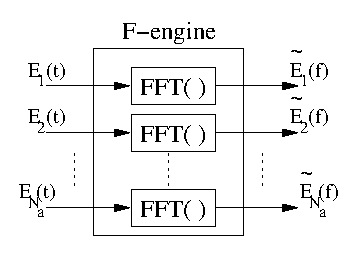
\includegraphics[width=\columnwidth]{figure4}
  % 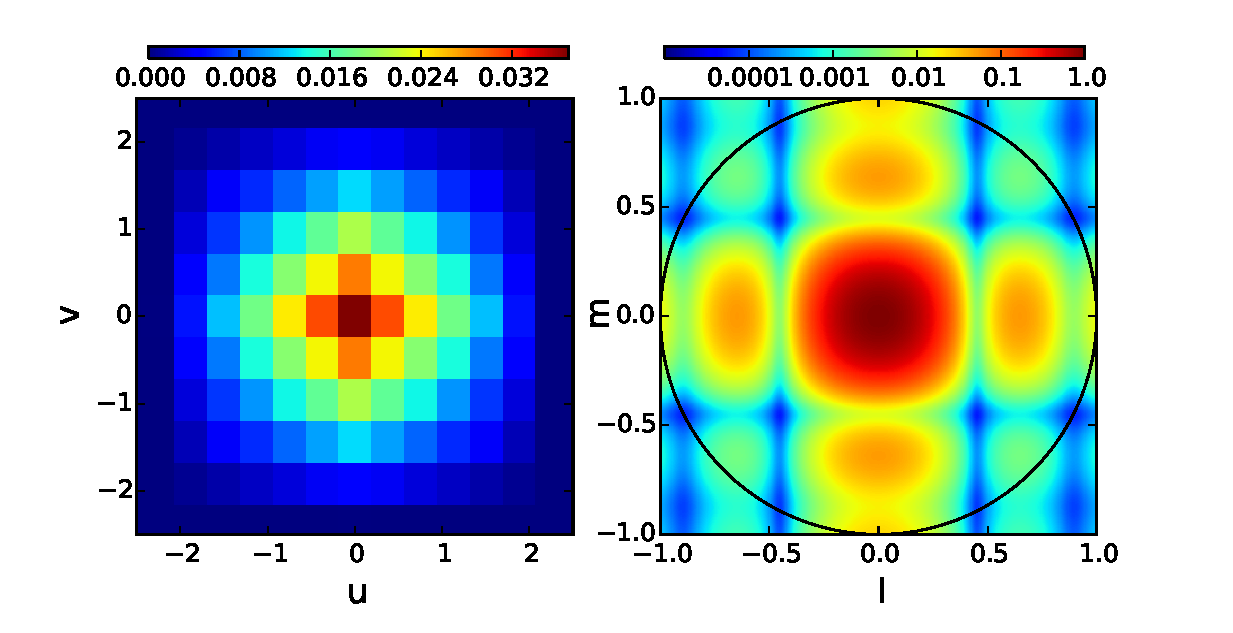
\includegraphics[width=\columnwidth]{autocorr_uvwts_pbeam}
  % 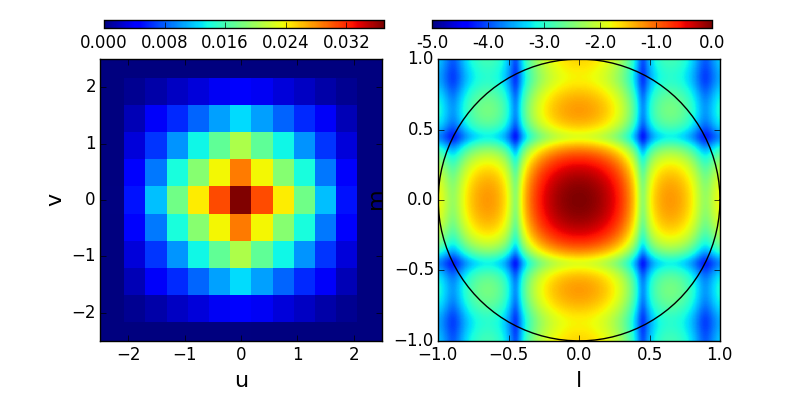
\includegraphics[width=\columnwidth]{autocorr_uvwts_pbeam.png}
  \caption{The auto-correlation of weights of a square shaped antenna aperture
    in the $uv$ plane (left) and the corresponding directional antenna power 
    response on the sky (right) in coordinates specified by direction cosines. 
    The antenna auto-correlation weights are normalized to a sum
    of unity yielding a peak response of unity in the antenna's directional
    power pattern on the sky. The color scale for the directional power 
    pattern is logarithmic. The black circle indicates the sky horizon and
    values beyond it are not physical and hence ignored.}
  \label{fig:autocorr_wts_PB}
\end{figure}

We inverse Fourier transform the squared images and beams back to the $uv$ plane and subtract the estimated auto-correlation kernel scaled to the peak value centred at the zero spacing pixel. The final averaged image is obtained by Fourier transforming the $uv$ plane data and weights with the auto-correlations subtracted to the image plane. These images are now comparable to those obtained from visibility-based imaging. This step of removing auto-correlations needs to be performed only once per integration time-scale and does not add significant cost to the full operation.

\subsection{Comparison of outputs}\label{sec:diff}

We investigate the two imaging algorithms for differences from the point of 
view of the quality of their outputs. We begin by comparing the images produced 
with the two approaches. 

Fig.~\ref{fig:MOFF-FX-image} shows the weighted dirty images (top) and synthesized beams (bottom) obtained with antenna-based MOFF and FX visibility-based imaging algorithms packaged in EPIC. The antenna auto-correlations that correspond to zero spacing have been removed from the correlated weights and data in the $uv$ plane, the MOFF image and the corresponding synthesized beam as described in \S\ref{sec:rm-autocorr}. The reconstructed sky image has the simulated sources at the expected sky positions in either case. Both algorithms result in images and synthesized beams that are well matched with each other. {\bf As expected, their fluxes are attenuated by a weighting proportional to the square of the antenna power pattern corresponding to a uniform square aperture.} 

\begin{figure}
  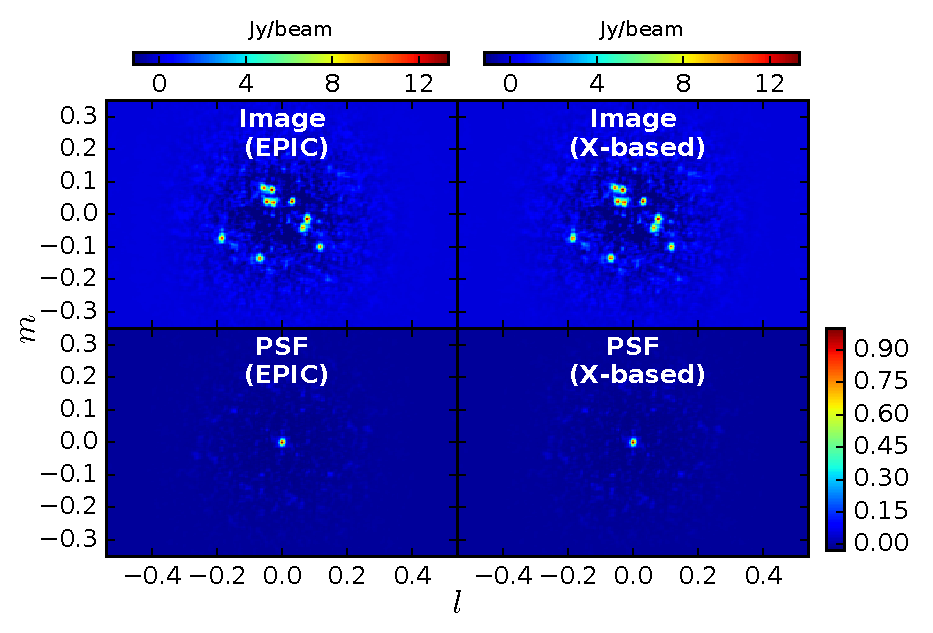
\includegraphics[width=\columnwidth]{figure5}
  % 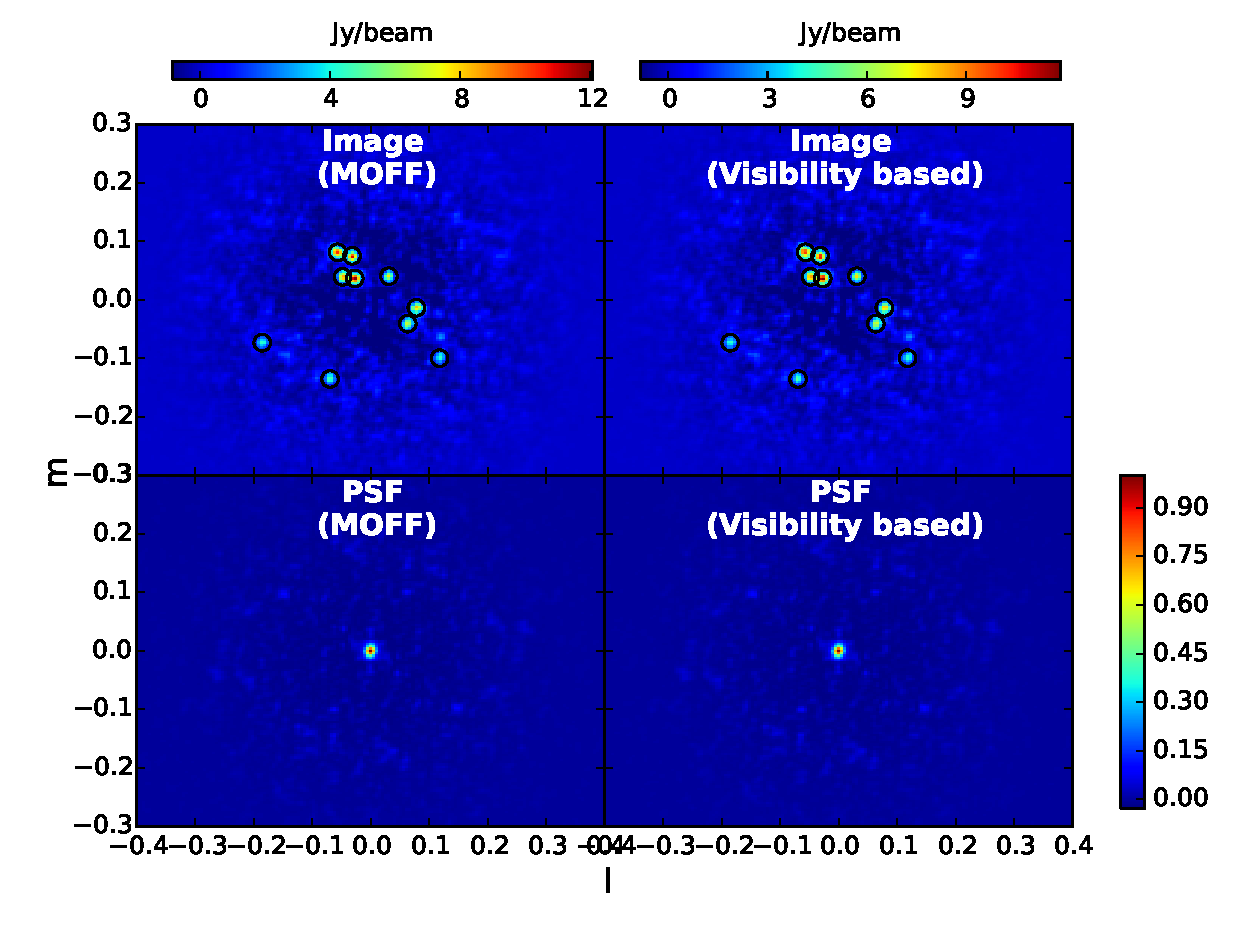
\includegraphics[width=\columnwidth]{MOFF_FX_comparison_10_random_source_positions_4_iterations_test_aperture_zoomed}
  % 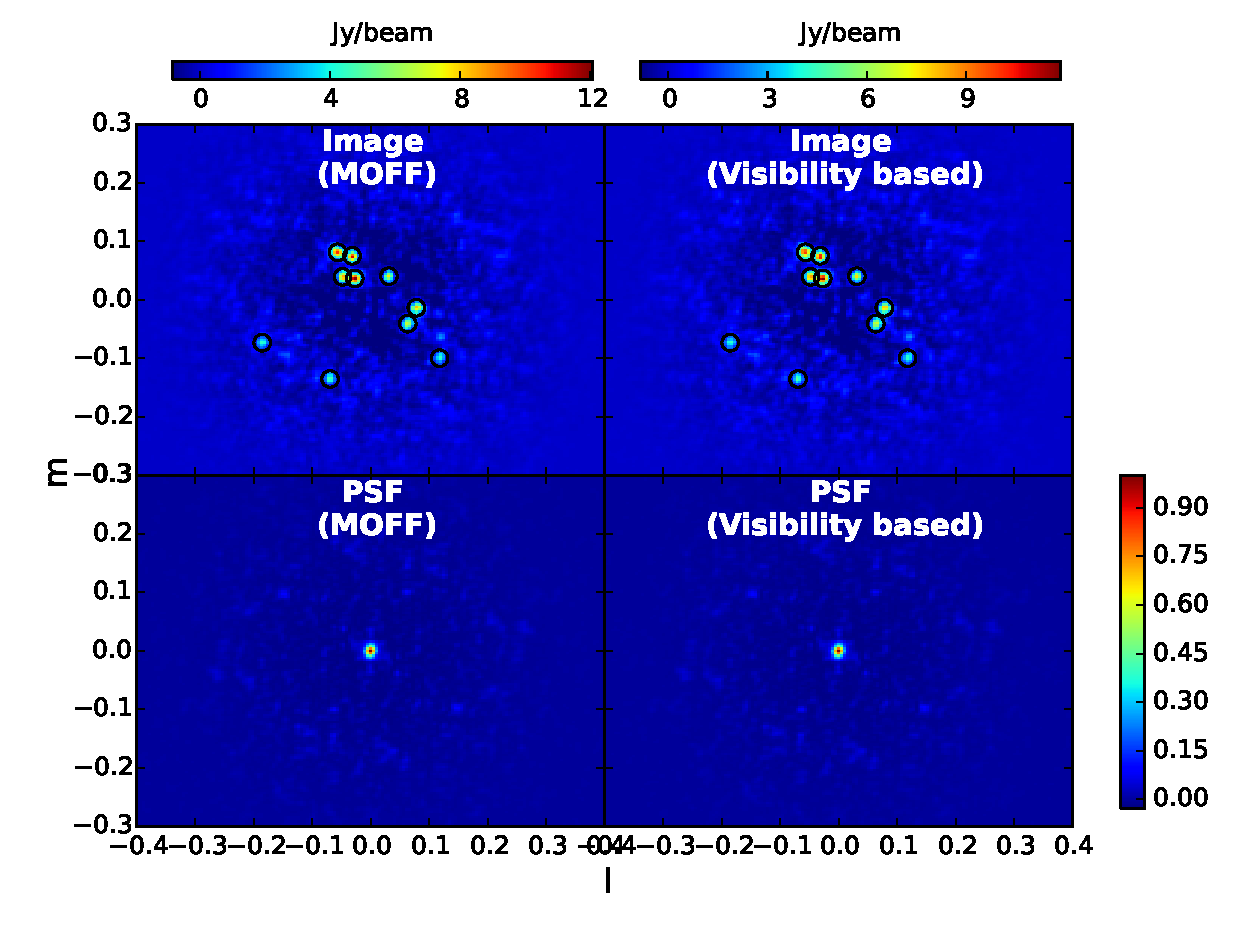
\includegraphics[width=\columnwidth]{MOFF_FX_comparison_10_random_source_positions_4_iterations_test_aperture_zoomed.eps}
  \caption{Weighted dirty images (top) and synthesized beams (bottom) obtained from simulated data using EPIC implementation of antenna-based MOFF algorithm (left) and visibility-based imaging (right). The antenna auto-correlations at zero-spacing have been removed from the MOFF images. The images in either case reconstruct the sources at the right locations with the fluxes attenuated expected after multiplication by the antenna power pattern {\bf squared}. The synthesized beams from the two algorithms are well matched in size and shape. The overall modulation by the power pattern is seen clearly in both images.}
  \label{fig:MOFF-FX-image}
\end{figure}

{\bf We examine in detail the respective synthesized beams in each case in Fig.~\ref{fig:MOFF-FX-psf-diff}. Slices at $m=0$ of the synthesized beams weighted by the antenna power pattern are shown for MOFF method using EPIC (solid black) and visibility-based (dashed gray) imaging. The two are found to match well. A magnified view shows that some differences at the level of $<0.5$\% exist in some regions. These are attributed to differences in the $uv$-plane antenna cross-correlation weights in the two methods which in turn arises due to the amount of coarseness in grid spacing as described below.}

\begin{figure}
  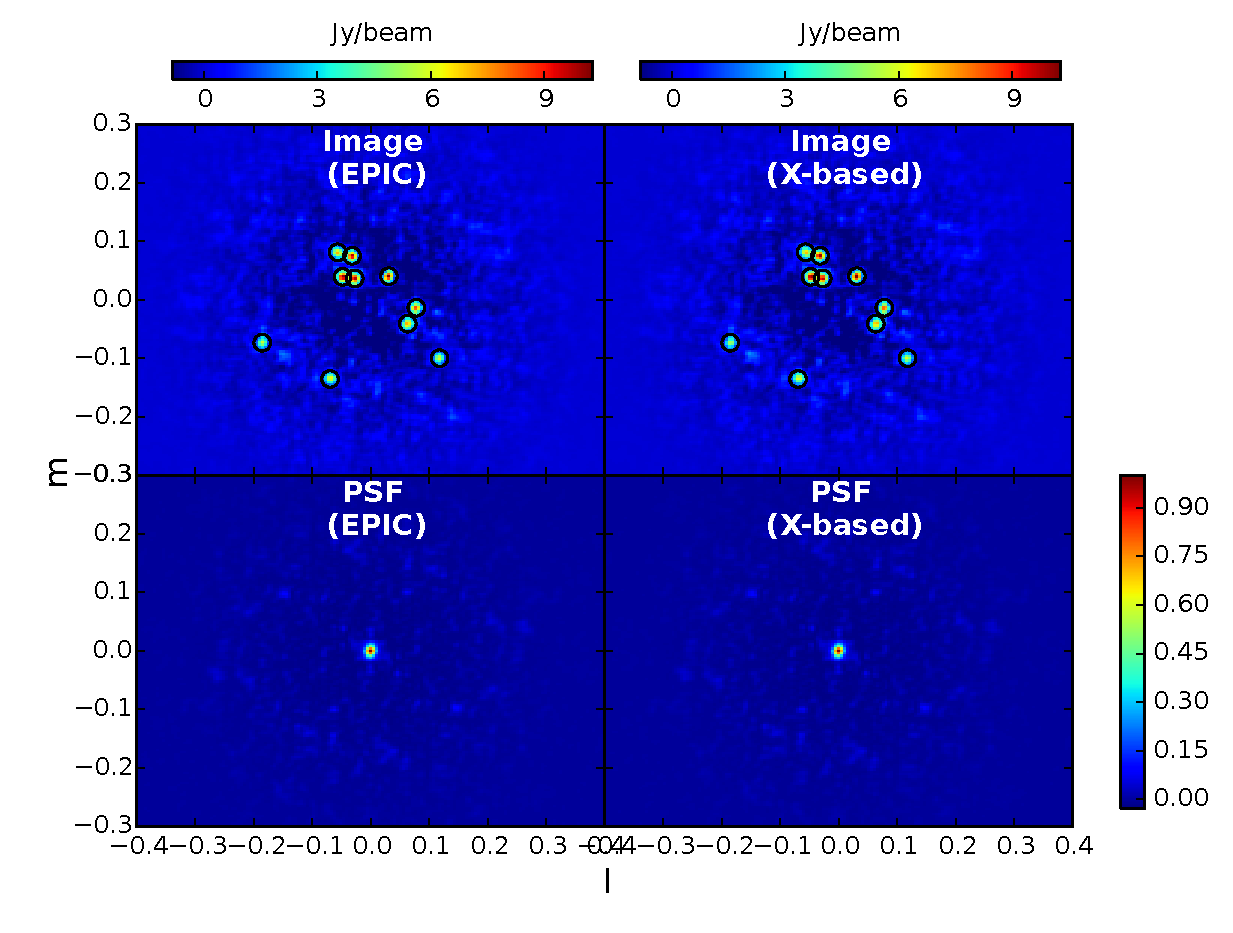
\includegraphics[width=\columnwidth]{figure6}
  \caption{{\bf Synthesized beams weighted by antenna power pattern sliced at $m=0$ obtained with MOFF algorithm using EPIC (solid black line) and visibility-based imaging (dashed gray line). The two appear almost identical. The inset provides a magnified view of differences in the synthesized beam slices between the two techniques at levels $\lesssim 0.5$\% relative to the peak. These are attributed to differences that arise in gridding and depends on the coarseness of the grid.}}
  \label{fig:MOFF-FX-psf-diff}
\end{figure}

{\bf The left panel of Fig.~\ref{fig:MOFF-FX-uvwts-diff} shows differences (in percentage relative to peak) in cross-correlated weights obtained with MOFF imaging in EPIC and visibility-based imaging. The maximum difference appears near the center of the $uv$-plane corresponding to antenna auto-correlations which have not been perfectly removed in the former. In other regions of the $uv$-plane, the differences are of the order of a few percent. The reason for these differences is described below.}

\begin{figure}
  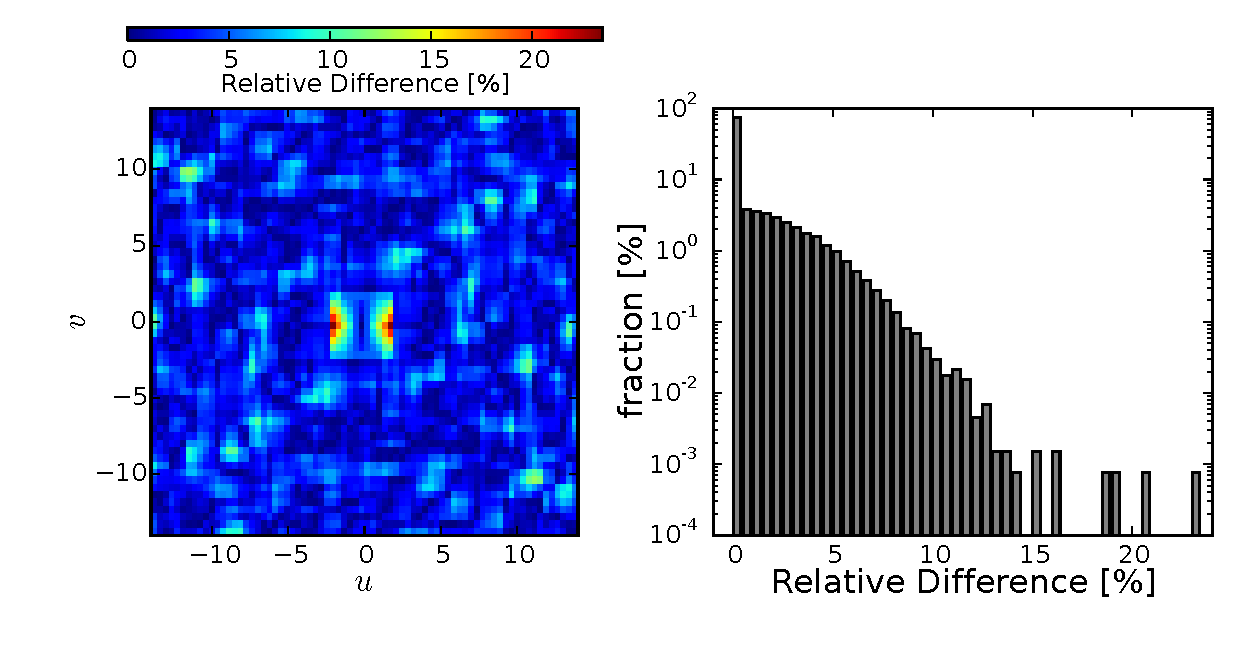
\includegraphics[width=\columnwidth]{figure7}
  % 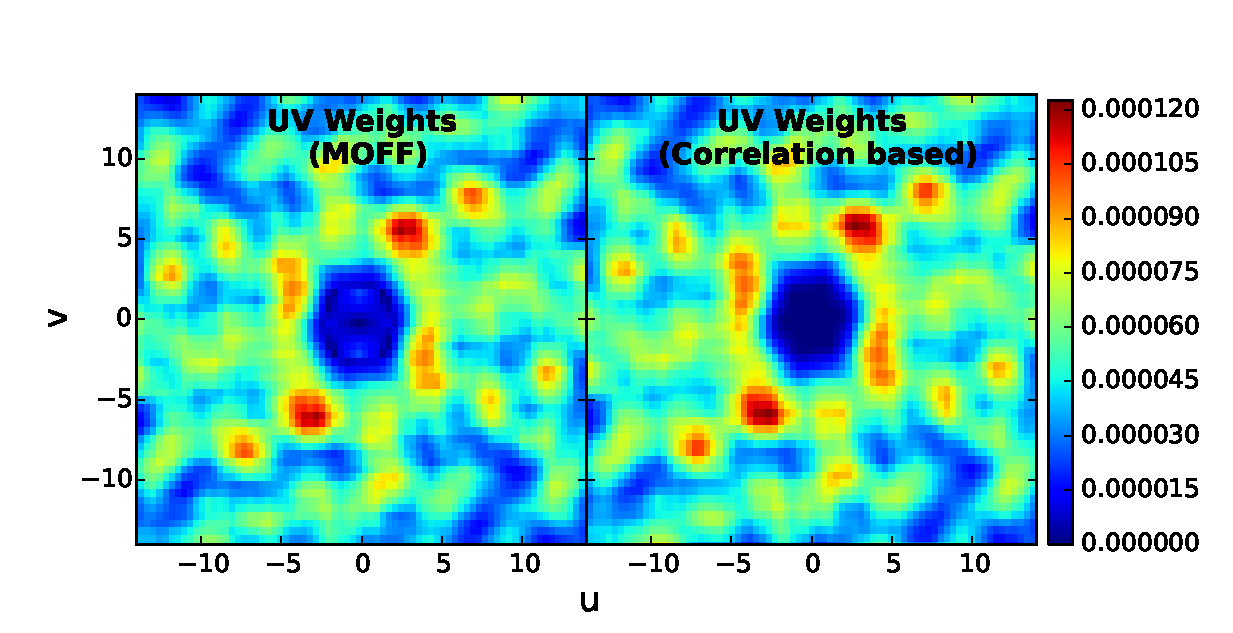
\includegraphics[width=\columnwidth]{MOFF_FX_comparison_uvwts_test_aperture_zero_spacing_removed}
  % 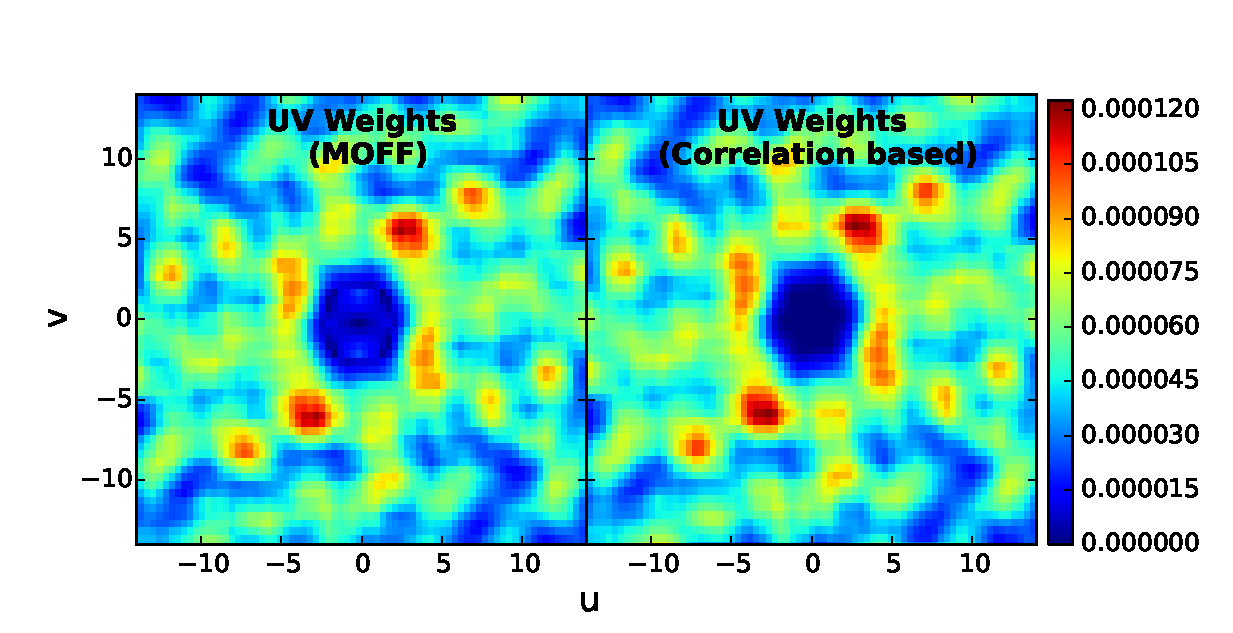
\includegraphics[width=\columnwidth]{MOFF_FX_comparison_uvwts_test_aperture_zero_spacing_removed.eps}
  \caption{{\bf {\it Left}: Differences (in \%) in cross-correlated weights in the $uv$ plane relative to the peak. The biggest difference ($\sim 20$\%) is found around the zero-spacing corresponding to auto-correlations of antenna weights due to gridding differences augmented by the relatively high number density of antenna auto-correlation footprints in that region. In most of the other regions, differences of the order of less than a few percent are seen. {\it Right}: Histogram (expressed as percentage) of the relative differences (in \%) between antenna cross-correlation weights shown on the left binned in intervals of 0.5\%. Over 70\% of the $uv$-cells do not differ by more than 0.5\% and over 90\% of $uv$-cells only differ by $<5$\% for the gridding coarseness used.}} 
  \label{fig:MOFF-FX-uvwts-diff}
\end{figure}

The gridding step in MOFF imaging samples the antenna footprint (either in analytic or lookup table formats) at the grid locations. Coverage of grid pixels by an antenna footprint may be $\sim 1$ pixel narrower particularly at the edge of the footprint along one or both directions relative to that from another identical antenna but with a fractionally different location relative to the grid. This depends on the exact location of the centre of the antenna relative to the grid and the coarseness of grid spacing. This first order loss of precision of the sampled footprint propagates to second order ($\sim 2$ pixels) upon correlation of the discretized weights. In other words, the correlated weights may suffer further loss of precision in their sampled footprint after correlation of two footprints each of which could be less precise to first order. On the other hand, in visibility-based imaging, a directly sampled $uv$ plane antenna power response (which is theoretically identical to the correlation of individual antenna footprints) centred on a baseline has a loss in precision at most to first order. Thus, although in the limit of infinitesimally small grid spacing they should be identical, the coarseness of grid spacing introduces subtle differences between the two.

These differences which are dependent on the coarseness of grid spacing can be mitigated by making the grid spacing finer at the expense of increased computational cost. Residuals centred around zero spacing can also be lowered by subtracting each auto-correlation of antenna weights separately by using the shape and extent of the sampled footprint appropriate for that specific antenna aperture. This is a general solution applicable even in case of heterogeneous antenna arrays and is under active development for EPIC.

We study the effect of the differences in gridded weights on the image plane. Fig.~\ref{fig:image-psf-diff} shows the difference between the synthesized beams obtained with the two methods. A difference map between the two synthesized beams is shown on the {\bf left}. The amplitude of the difference appears to be modulated by the directional power response of the antenna. {\bf On the right}, in radial bins, the rms of the synthesized beam (gray) and the rms of the difference map (black) are plotted in percentage units relative to the peak (to be read using the axis on the left side of the plot). The antenna power pattern (red; to be read using the scale on the right) is plotted for reference. 

\begin{figure}
  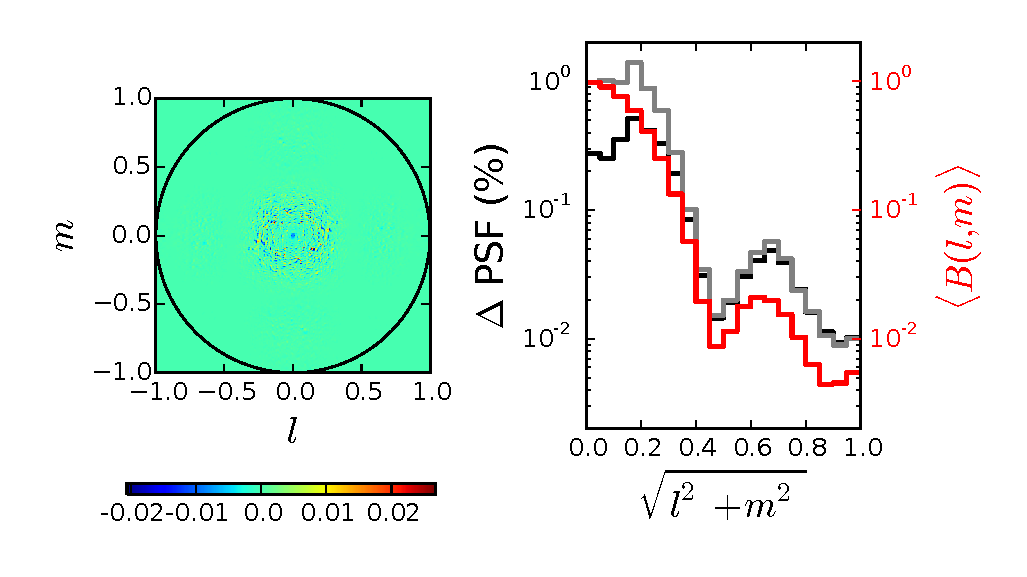
\includegraphics[width=\columnwidth]{figure8}
  % 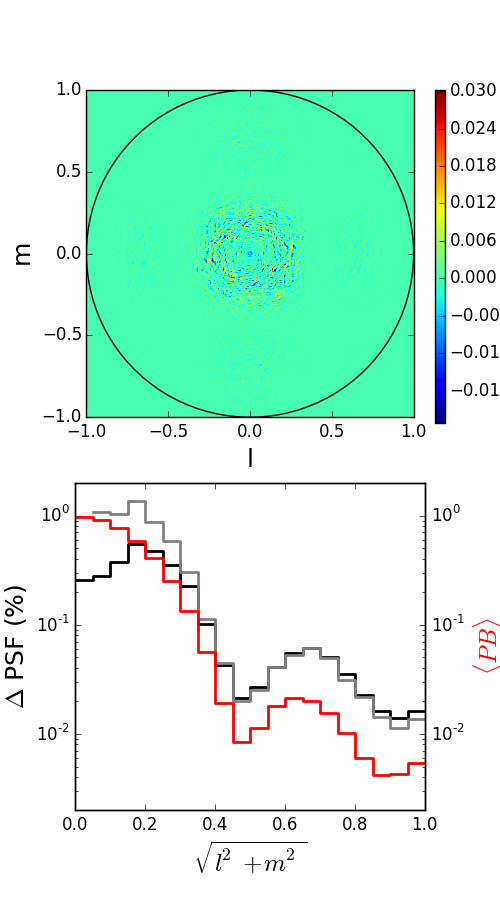
\includegraphics[width=\columnwidth]{diff_psf_MOFF-FX_test_aperture}
  % 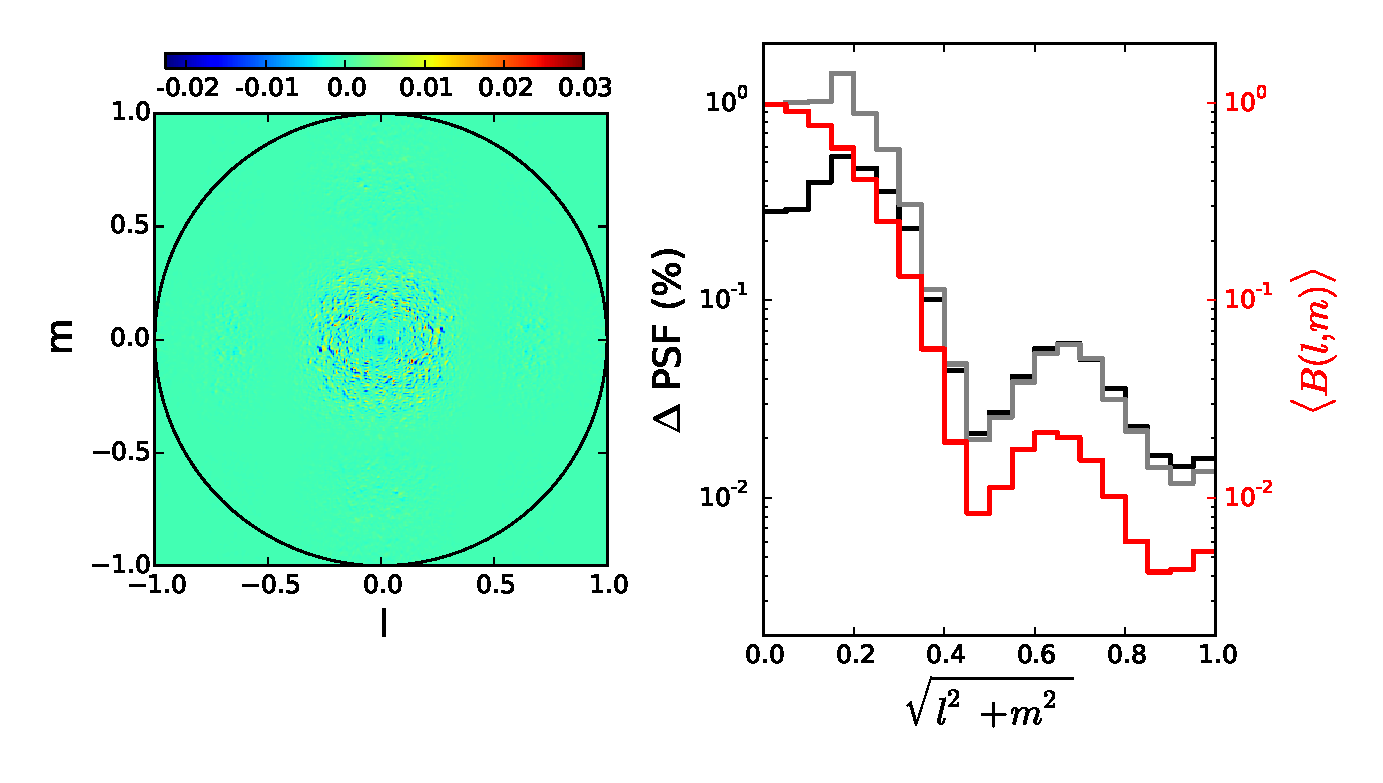
\includegraphics[width=\columnwidth]{diff_psf_MOFF-FX_test_aperture.eps}
  \caption{Map of difference between the synthesized beams obtained with the 
    two methods (left) and radial statistics of the synthesized beams and 
    their differences (right). The radial variations of rms of the synthesized 
    beam (gray) and that of the rms of the difference (black) are shown as 
    percentage of the peak synthesized beam. Radially averaged directional 
    antenna power response in absolute scale is shown in red and is to be read 
    with the scale on the right side of the axis. The maximum difference is of 
    the order of a few percent. Amplitude of the rms of the difference is 
    modulated by the power pattern of the antenna.}
  \label{fig:image-psf-diff}
\end{figure}

The synthesized beam rms is proportional to the antenna power pattern as 
expected from a point spread function uncorrected for the antenna power pattern. 
The rms of differenced synthesized beams is also modulated by the antenna power 
pattern. The rms of the difference is definitely lesser than the rms of the 
synthesized beam in the central regions up to $(l^2+m^2)^{1/2}\lesssim 0.3$. This 
implies that the beams are well matched in the central regions. In the outer 
regions, their mismatch is comparable to the rms of synthesized beams. These findings are consistent with Fig.~\ref{fig:MOFF-FX-psf-diff}. This 
indicates the two synthesized beams are not randomly different from 
each other in which case the rms of the difference would have been 
$\approx \sqrt{2}$ higher than the rms of the each of the synthesized beams. 
This {\bf means} that while differences exist, large fractions of them are still 
well matched to each other even out to the horizon. Thus the rounding errors in 
gridding do not affect the statistics of the images or the synthesized beams.

\subsection{Application to LWA data}\label{sec:LWA-data}

Here we demonstrate our software using narrow band data from the LWA station 
in New Mexico. This data is in LWA narrow-band transient buffer (TBN) format 
from 255 antennas within roughly a diameter of 100~m. The data is centred at a 
frequency of 74.03~MHz, with a sample rate (equal to the bandwidth) of 100~kHz 
with 512 complex time samples per antenna in a A/D writeout time-scale of 
5.12~ms, a frequency resolution of 195.3125~Hz and dual polarization. There are 
391 such writeouts (or time stamps; each contains 512 time samples at 100~kHz 
sampling) yielding a total duration of 2~s. 

We corrected the cable delays, but otherwise assume the data is sufficiently calibrated to image directly. A detailed demonstration of EPICal on this data is presented in \citet{bea16}.

Fig.~\ref{fig:LWA-image} shows the image produced with MOFF imaging 
packaged in EPIC after averaging over $\approx$~20~ms (four writeouts) of data 
and the inner $\approx 80$ per cent of bandwidth (roughly 80~kHz). The image is 
shown in direction cosine coordinates -- $l$ along the horizontal axis and $m$ 
along the vertical axis. The flux scale is arbitrary. Even in this 
proof-of-concept demonstration, we see Cyg~A and Cas~A prominently as annotated, 
thus validating the functionality of EPIC.

\begin{figure}
  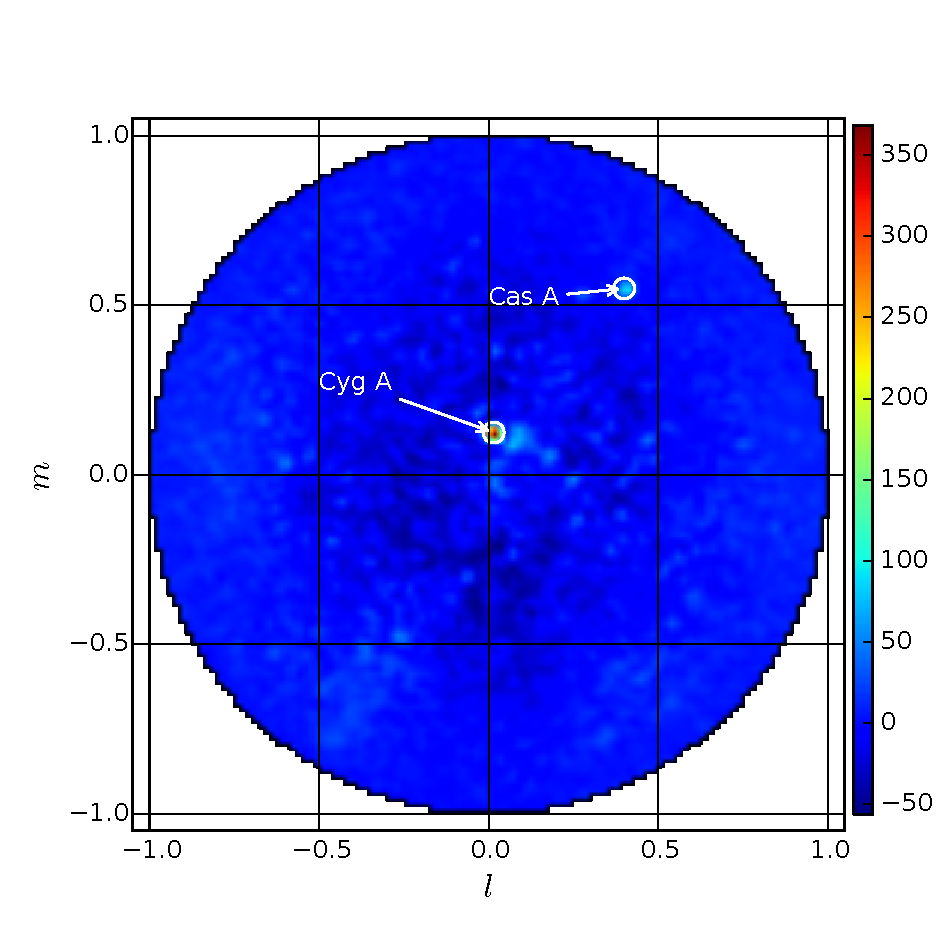
\includegraphics[width=\columnwidth]{figure9}
  % 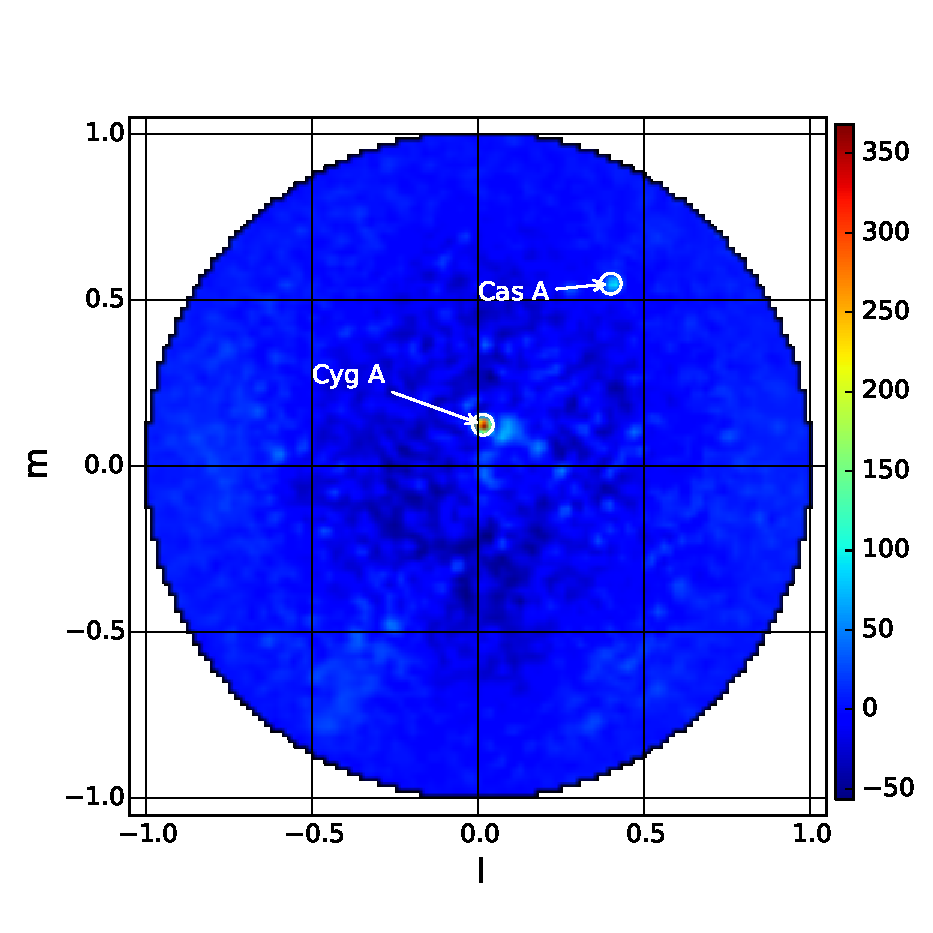
\includegraphics[width=\columnwidth]{LWA_MOFF_bandavg_image_4_iterations_analytic_aperture}
  % 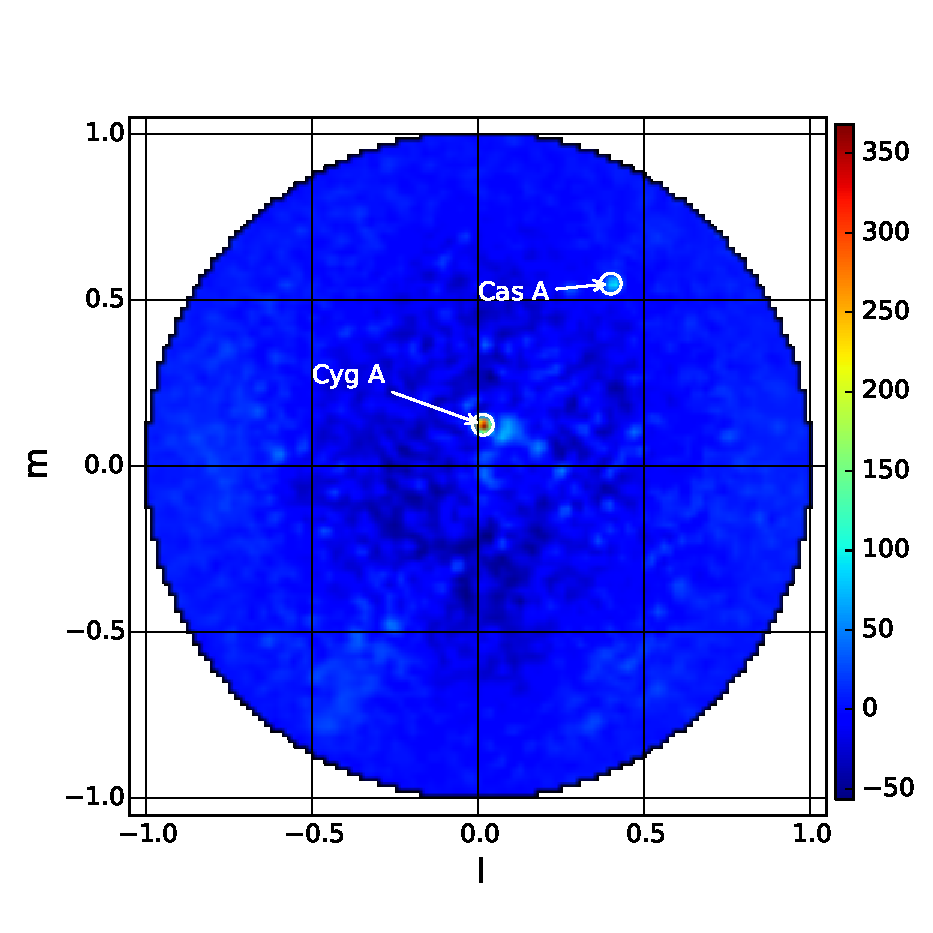
\includegraphics[width=\columnwidth]{LWA_MOFF_bandavg_image_4_iterations_analytic_aperture.eps}
  \caption{Image from LWA TBN data obtained with MOFF imaging using EPIC 
    package after averaging over 20~ms and $\approx 80$~kHz. The x- and y-axes
    denote direction cosines $l$ and $m$ respectively. The antenna voltages
    are compensated for their respective delays. The flux scale is arbitrary.
    Locations of Cyg~A and Cas~A are annotated.}
  \label{fig:LWA-image}
\end{figure}

\section{Imaging with Heterogeneous Antenna Arrays}\label{sec:versatility}

{\bf One of the advanced features of the MOFF algorithm and its implementation via EPIC is the ability to naturally account for heterogeneity of antennas while still producing images with maximal information \citep{mor11}. Unlike the assumption frequently made in standard radio interferometry that all antennas are identical, EPIC can implement the most generic case where no such assumption can be made. In other words, EPIC does not assume $W_a(\mathbf{r}-\mathbf{r}_a)$ or $B_{ab}(\mathbf{r}-\mathbf{r}_{ab})$ for different antennas are identical. However, any {\it a priori} knowledge available that certain sets of antennas have identical illumination patterns can be easily passed on to EPIC to avoid redundant computations and thus increase efficiency.

We present a methodology to understand the effective angular weighting in the image obtained with EPIC from a heterogeneous array and compare it with that from standard interferometry which assumes a homogeneous array (all antennas are identical). We also demonstrate how the assumption in the latter results in a mis-estimation of the recovered sky model.

Dropping the noise term and time dependence, the visibility measured by an antenna pair can be written from equation~\ref{eqn:measurement-eqn-1} as:
\begin{align}\label{eqn:measurement-eqn-2}
  V_{ab}(f) &= \int \mathcal{W}^\textrm{I}_a(\hat{\mathbf{s}},f)\mathcal{W}^{\textrm{I}\star}_b(\hat{\mathbf{s}},f)\,\mathcal{I}(\hat{\mathbf{s}},f)\,e^{-2\pi i f\mathbf{r}_{ab}\!\cdot\,\hat{\mathbf{s}}/c}\,\dif\Omega,
\end{align}
where, superscript `$\textrm{I}$' in the $\mathcal{W}$ term indicates the weighting is inherently introduced by the instrument during the measurement process. The beam-weighted dirty image is:
\begin{align}
  \mathcal{I}_\textrm{D}(\hat{\mathbf{s}},f) &= \frac{1}{\Nant(\Nant-1)/2}\,\sum_{ab}\, V_{ab}(f)\,e^{2\pi i f\mathbf{r}_{ab}\!\cdot\,\hat{\mathbf{s}}/c},
\end{align}
{\bf where, we have assumed equal weighting for each antenna pair}.

When the array is homogeneous, $\mathcal{W}^\textrm{I} \equiv \mathcal{W}^\textrm{I}_a \equiv \mathcal{W}^\textrm{I}_b$ and the above equation reduces to:
\begin{align}\label{eqn:dirty-image-homogeneous}
  \mathcal{I}_\textrm{D}(\hat{\mathbf{s}},f) &= |\mathcal{W}^\textrm{I}(\hat{\mathbf{s}},f)|^2\,\mathcal{I}_\textrm{D}^\textrm{iso}(\hat{\mathbf{s}},f),
\end{align}
where, $\mathcal{I}_\textrm{D}^\textrm{iso}(\hat{\mathbf{s}},f)$ is the dirty image with no beam weighting (isotropic, uniform weighting {\bf of the sky}) determined only by the array layout and $|\mathcal{W}^\textrm{I}|^2$ is the directional power pattern of the antenna pair familiar in standard interferometry.

{\bf In order to understand an image from a heterogeneous array, we start by looking at the contribution to the image from the visibility, $V_{ab}$, from each antenna pair.} While imaging, EPIC introduces a weighting to each antenna during gridding as given by equations~\ref{eqn:dirty-image-FX} and \ref{eqn:e-field-conv}, and equivalently, the weighted visibility from {\bf an} antenna pair $ab$ projected on the grid is:
\begin{align}
  V^\prime_{ab}(\mathbf{r},f) &= B^{\textrm{G}\star}_{ab}(\mathbf{r}-\mathbf{r}_{ab},f)\,V_{ab},
\end{align}
where, $B^\textrm{G}_{ab}(\mathbf{r}-\mathbf{r}_{ab},f)$ is obtained by the spatial cross-correlation of weighting kernels associated with the individual antennas using the definition:
\begin{align}
  B^\textrm{G}_{ab}(\mathbf{r}-\mathbf{r}_{ab},f) &= \int W^\textrm{G}_a(\mathbf{r}^\prime-\mathbf{r}_a)\,W^{\textrm{G}\star}_b(\mathbf{r}^\prime+\mathbf{r}-\mathbf{r}_b)\,\dif^2\mathbf{r}^\prime.
\end{align}
The superscript `$\textrm{G}$' denotes the weighting introduced in analysis during the gridding process. Optimal imaging requires $W^\textrm{G}_a = W^\textrm{I}_a$ \citep{mor09,mor11}. However, we keep the two superscripts separately to describe output images under the wrong assumption that the array is homogeneous when instead it is actually heterogeneous.

The sky response of the weighted visibility is:
\begin{align}
  \mathcal{I}^\prime_{ab}(\hat{\mathbf{s}},f) &= \int V^\prime_{ab}(\mathbf{r},f)\,e^{2\pi i f\mathbf{r}\cdot\,\hat{\mathbf{s}}/c}\,\dif^2\mathbf{r} \nonumber\\
                                              &= \int B^{\textrm{G}\star}_{ab}(\mathbf{r}-\mathbf{r}_{ab},f)\,V_{ab}\,e^{2\pi i f\mathbf{r}\cdot\,\hat{\mathbf{s}}/c}\,\dif^2\mathbf{r} \nonumber\\
                                              &= V_{ab}\,\int \left[\int W^{\textrm{G}\star}_a(\mathbf{r}^\prime-\mathbf{r}_a)\,W^\textrm{G}_b(\mathbf{r}^\prime+\mathbf{r}-\mathbf{r}_a)\,\dif^2\mathbf{r}^\prime\right] \nonumber\\
                                              &\qquad\qquad \times e^{2\pi i f\mathbf{r}\cdot\,\hat{\mathbf{s}}/c}\,\dif^2\mathbf{r} \nonumber\\
                                              &= \mathcal{W}^{\textrm{G}\star}_a(\hat{\mathbf{s}},f)\mathcal{W}^\textrm{G}_b(\hat{\mathbf{s}},f)\,V_{ab}\,e^{2\pi i f\mathbf{r}_{ab}\!\cdot\,\hat{\mathbf{s}}/c},
\end{align}
which denotes the fringe from the weighted visibility. The image output of EPIC is equivalent to averaging these weighted fringes from all antenna pairs:
\begin{align}\label{eqn:wt-dirty-image-EPIC}
  \mathcal{I}^\prime(\hat{\mathbf{s}},f) &= \frac{1}{\Nant(\Nant-1)/2}\,\sum_{\substack{ab\\a\ne b}}\,\mathcal{I}^\prime_{ab}(\hat{\mathbf{s}},f) \nonumber\\
                                         &= \frac{1}{\Nant(\Nant-1)/2}\,\sum_{\substack{ab\\a\ne b}}\,\left[\mathcal{W}^{\textrm{G}\star}_a(\hat{\mathbf{s}},f)\mathcal{W}^\textrm{G}_b(\hat{\mathbf{s}},f)\,V_{ab}\right. \nonumber\\
  &\qquad\qquad\qquad\qquad\qquad\qquad \times \left. e^{2\pi i f\mathbf{r}_{ab}\!\cdot\,\hat{\mathbf{s}}/c}\right].
\end{align}

If all antennas are identically weighted ($W^\textrm{G} \equiv W^\textrm{G}_a \equiv W^\textrm{G}_b$), using equation~\ref{eqn:dirty-image-homogeneous}, equation~\ref{eqn:wt-dirty-image-EPIC} reduces to: 
\begin{align}\label{eqn:wt-dirty-image-homogeneous}
  \mathcal{I}^\prime(\hat{\mathbf{s}},f) &= \frac{\left|\mathcal{W}^\textrm{G}(\hat{\mathbf{s}},f)\right|^2}{\Nant(\Nant-1)/2}\,\sum_{\substack{ab\\a\ne b}}\,V_{ab}\,e^{2\pi i f\mathbf{r}_{ab}\!\cdot\,\hat{\mathbf{s}}/c} \nonumber\\
  &= \left|\mathcal{W}^\textrm{G}(\hat{\mathbf{s}},f)\right|^2\,\mathcal{I}_\textrm{D}(\hat{\mathbf{s}},f) \nonumber\\
  &= \left|\mathcal{W}^\textrm{G}(\hat{\mathbf{s}},f)\right|^2\,\left|\mathcal{W}^\textrm{I}(\hat{\mathbf{s}},f)\right|^2\,\mathcal{I}_\textrm{D}^\textrm{iso}(\hat{\mathbf{s}},f).
\end{align}
Thus, the dirty image, which is already attenuated by the instrumental power pattern, gets further attenuated by the power pattern introduced in the gridding step in EPIC imager. This is consistent with \citet{mor09}. 

{\bf We note that all quantities in the celestial plane (calligraphic fonts) are functions of position, $\hat{\mathbf{s}}$, and frequency, $f$. For convenience, we drop writing this dependence explicitly hereafter.}

{\bf For a heterogeneous array, it is necessary to keep track of antennas and antenna pairs of different types which will determine the final weighting in the synthesized image.} We consider a heterogeneous array consisting of a total of $\Nant$ antennas under $N_\textrm{T}$ different types. And under each antenna type $i$, there are $n_i$ antennas such that $\sum_i n_i = \Nant$. The total number of unique non-zero spacing antenna pairs is $\Nant(\Nant-1)/2$ and there are potentially up to $N_\textrm{T}(N_\textrm{T}+1)/2$ unique antenna pair types obtained by pairwise combination of the $N_\textrm{T}$ antenna types. Thus, the total number of antenna pairs, 
\begin{align}\label{eqn:total-baselines}
  \frac{1}{2}\Nant(\Nant-1) &= \frac{1}{2}\,\sum_{ij} n_{ij}, \\
  \textrm{where}, \quad   n_{ij} &= \begin{cases}
    n_i\,n_j, & i\ne i \\
    n_i(n_i-1), & i=j, 
  \end{cases}
\end{align}
is obtained by counting antenna pairs, $n_{ij}$, in different antenna pair types, $ij$.

Since equation~\ref{eqn:wt-dirty-image-EPIC} is obtained by averaging weighted fringes over all unique antenna pairs, it can be expressed as: 
\begin{align}\label{eqn:wt-dirty-image-EPIC-decomp}
  \mathcal{I}^\prime &= \frac{1/2}{\Nant(\Nant-1)/2}\,\sum_{ij}\sum_{\substack{ab\\a\ne b\\a\in i, b\in j}}\,\mathcal{I}^\prime_{ab}
\end{align}
Here, equation~\ref{eqn:wt-dirty-image-EPIC} has been decomposed as the sum of fringes over all unique antenna pairs in an antenna pair type (inner sum) and subsequently summed over all antenna pair types (outer sum). 

For purposes of demonstration in this study, we make the following simplification. We assume that the spatial distribution of antenna pairs in each antenna pair type are similar and thus result in a similar dirty image, $\mathcal{I}_\textrm{D}^\textrm{iso}$. This usually holds when $\Nant$ is large and antennas under each antenna type are chosen randomly such that differences in the point spread functions are insignificant. Under this assumption, equation~\ref{eqn:wt-dirty-image-EPIC-decomp} can be written as:
\begin{align}\label{eqn:wt-dirty-image-EPIC-decomp-approx1}
  \mathcal{I}^\prime &\approx \frac{\mathcal{I}_\textrm{D}^\textrm{iso}}{\Nant(\Nant-1)}\,\sum_{ij}\sum_{\substack{ab\\a\ne b\\a\in i, b\in j}} \mathcal{W}^{\textrm{G}\star}_a\,\mathcal{W}^\textrm{G}_b\,\mathcal{W}^\textrm{I}_a\,\mathcal{W}^{\textrm{I}\star}_b,
\end{align}
where, $\mathcal{I}_\textrm{D}^\textrm{iso}$ is approximately the same for all terms and has been pulled outside the summations. For all antennas indexed by $a$ that belong to a particular type $i$, we replace $\mathcal{W}_a$ with $\mathcal{W}_{(i)}$ {\bf and is applicable to those arising} from both instrumental (superscript `$I$') and gridding (superscript `$G$') origins. Using arguments similar to those in equation~\ref{eqn:total-baselines}, equation~\ref{eqn:wt-dirty-image-EPIC-decomp-approx1} can be further simplified to:
\begin{align}\label{eqn:wt-dirty-image-EPIC-decomp-approx2}
  \mathcal{I}^\prime &\approx \frac{\mathcal{I}_\textrm{D}^\textrm{iso}}{\Nant(\Nant-1)}\,\sum_{ij}n_{ij}\,\mathcal{W}^{\textrm{G}\star}_{(i)}\,\mathcal{W}^\textrm{G}_{(j)}\,\mathcal{W}^\textrm{I}_{(i)}\,\mathcal{W}^{\textrm{I}\star}_{(j)}.
\end{align}
Then the effective attenuation of the dirty image due to instrumental and gridding weights is:
\begin{align}\label{eqn:effective-weighting}
  \mathcal{W}_\textrm{eff} &= \mathcal{I}^\prime\, / \,\mathcal{I}_\textrm{D}^\textrm{iso}.
\end{align}
This means that the effective attenuation of the dirty image is obtained by combinations of the fourth power of antenna voltage patterns each weighted by the number of antenna pairs in those antenna pair types. In an optimally weighted image, $\mathcal{W}^\textrm{G}_{(i)} \equiv \mathcal{W}^\textrm{I}_{(i)}$ and thus, equation~\ref{eqn:effective-weighting} reduces to:
\begin{align}\label{eqn:effective-weighting-optimal}
  \mathcal{W}_\textrm{eff}^\textrm{opt} &\approx \frac{1}{\Nant(\Nant-1)}\,\sum_{ij} n_{ij}\,\left|\mathcal{W}^\textrm{I}_{(i)}\right|^2\left|\mathcal{W}^\textrm{I}_{(j)}\right|^2,
\end{align}
where the superscript `$\textrm{opt}$' denotes `optimal'.

For purposes of illustration, we consider a simple scenario in which there are two antenna types each containing roughly equal numbers of antennas with similar layouts but the analysis is performed under the wrong assumption that all antennas are identical and are all of the first type. In an optimally weighted image, the optimal effective weighting given by equation~\ref{eqn:effective-weighting-optimal} will be:
\begin{align}\label{eqn:effective-weighting-optimal-example}
  \mathcal{W}_\textrm{eff}^\textrm{opt} &\approx \frac{1}{\Nant(\Nant-1)}\,\left[n_1(n_1-1)\,\left|\mathcal{W}^\textrm{I}_{(1)}\right|^4 \right.\nonumber\\
  &\qquad\qquad\qquad\qquad + n_2(n_2-1)\,\left|\mathcal{W}^\textrm{I}_{(2)}\right|^4 \nonumber\\
  &\qquad\qquad\qquad\qquad \left. + n_1n_2\,\left|\mathcal{W}^\textrm{I}_{(1)}\right|^2\,\left|\mathcal{W}^\textrm{I}_{(2)}\right|^2\right].
\end{align}
On the other hand, $\mathcal{W}^\textrm{G}_{(1)} = \mathcal{W}^\textrm{I}_{(1)}$ and $\mathcal{W}^\textrm{G}_{(2)} = \mathcal{W}^\textrm{I}_{(1)}$ for an image obtained in the erroneous case in which all antennas are assumed to be identical. It will be sub-optimal with effective weighting:
\begin{align}\label{eqn:effective-weighting-suboptimal-example}
  \mathcal{W}_\textrm{eff}^\textrm{sub} &\approx \frac{1}{\Nant(\Nant-1)}\,\left[n_1(n_1-1)\,\left|\mathcal{W}^\textrm{I}_{(1)}\right|^4\right.\nonumber\\
  &\qquad\qquad\qquad\qquad + n_2(n_2-1)\,\left|\mathcal{W}^\textrm{I}_{(1)}\right|^2\,\left|\mathcal{W}^\textrm{I}_{(2)}\right|^2 \nonumber\\
  &\qquad\qquad\qquad\qquad \left. + n_1n_2\,\left|\mathcal{W}^\textrm{I}_{(1)}\right|^2 \,\mathcal{W}^\textrm{I}_{(1)}\,\mathcal{W}^{\textrm{I}\star}_{(2)}\right].
\end{align}
Finally, since no {\it a priori} information will be available about the heterogeneous array in case of the erroneous assumption, the effective weighting in the image will be believed to be $\mathcal{W}_\textrm{eff}^\textrm{err} = \left|\mathcal{W}_{(1)}^\textrm{I}\right|^4$. 

Estimates of the dirty images with uniform, isotropic weighting in the optimal and erroneous cases will be obtained by dividing the respective weighted images by their assumed effective weights $\mathcal{W}_\textrm{eff}^\textrm{opt}$ and $\mathcal{W}_\textrm{eff}^\textrm{err}$ respectively as:
\begin{align}
  \widehat{\mathcal{I}}_\textrm{D}^\textrm{iso} &\approx \begin{cases}
    \mathcal{I}_\textrm{D}^\textrm{iso} &\textrm{, \qquad optimal case} \\
    \mathcal{I}_\textrm{D}^\textrm{iso}\,\frac{\mathcal{W}_\textrm{eff}^\textrm{sub}}{\mathcal{W}_\textrm{eff}^\textrm{err}} &\textrm{, \qquad erroneous case}
  \end{cases}
\end{align}

If $\mathcal{I}_\textrm{M}$ is the sky model, then $\mathcal{I}_\textrm{D}^\textrm{iso}$ can be expressed as:
\begin{align}\label{eqn:img-uncertainties}
  \mathcal{I}_\textrm{D}^\textrm{iso} &= \mathcal{I}_\textrm{M} + \delta\mathcal{I}_\textrm{S} + \delta\mathcal{I}_\textrm{M},
\end{align}
where the second and third terms on the right hand side denote fluctuations due to sidelobes and those intrinsic to the model, respectively. We define the normalized estimates of the sky model $\widehat{\mathcal{I}}_\textrm{M}^\textrm{norm} \equiv \widehat{\mathcal{I}}_\textrm{D}^\textrm{iso} / \mathcal{I}_\textrm{M}$. Ideally, $\widehat{\mathcal{I}}_\textrm{M}^\textrm{norm}$ should be consistent with unity and not exceed beyond levels of uncertainty as determined by equation~\ref{eqn:img-uncertainties}.

In our simulations, the antenna layout, duration of observation, center frequency and bandwidth used are the same as in \S\ref{sec:sim}. Antennas have square apertures. Those of the first and second types, which have roughly equal numbers of antennas with similar layouts, have 1.1~m and 6.6~m on their sides respectively. $\mathcal{I}_\textrm{M}$ consists of point sources of random flux densities brighter than 10~Jy along westward and south-westward directions as seen in Fig.~\ref{fig:nonphysical-image}, which shows an optimally weighted image, $\mathcal{I}^\prime$, obtained with EPIC using the MOFF algorithm after averaging over the entire bandwidth and duration of simulated observation. 

\begin{figure*}
\subfloat[][Optimally weighted EPIC image]{\label{fig:nonphysical-image}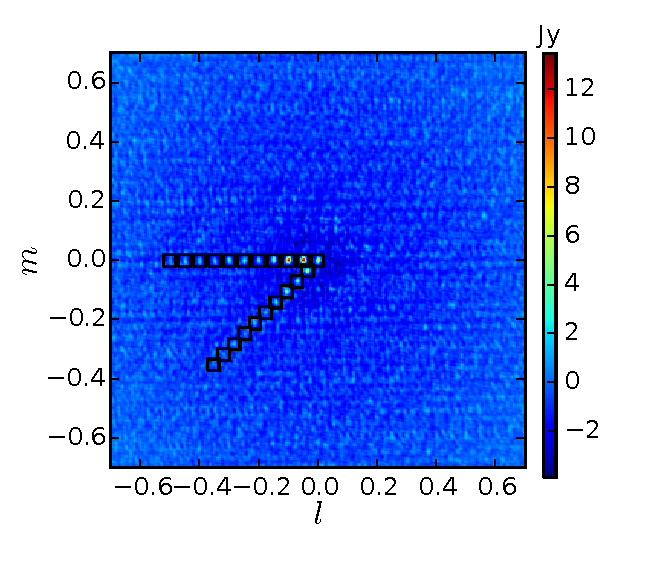
\includegraphics[width=0.5\linewidth]{figure10a.eps}}
\subfloat[][Estimates of normalized radial flux density profile]{\label{fig:norm-flux-density}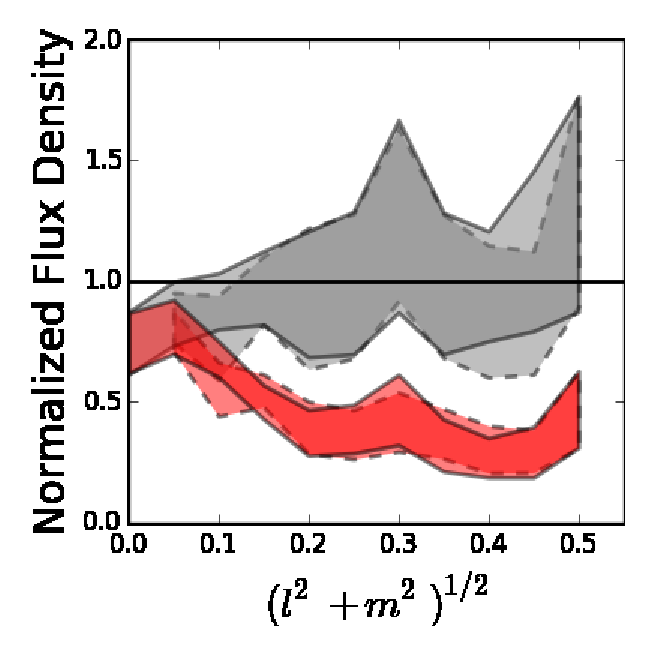
\includegraphics[width=0.42\linewidth]{figure10b.eps}}
\caption{{\bf (a)~Optimally weighted image, $\mathcal{I}^\prime$, of simulated sky model obtained by EPIC using MOFF algorithm after averaging over entire bandwidth and duration of simulated observation. 51 antennas in the inner core of the MWA layout were used with uniformly illuminated square apertures. Roughly half of them were squares with 1.1~m sides (first type) and the rest with 6.6~m (second type). Point sources were simulated along westward and south-westward directions with random flux densities brighter than 10~Jy. Black boxes shown around point sources are for purposes of collecting image statistics. (b)~Normalized flux density estimates, $\widehat{\mathcal{I}}_\textrm{M}^\textrm{norm}$, as a function of distance from image center. Bands indicate an approximate ``$1\sigma$'' uncertainty arising from sidelobe confusion and intrinsic randomness of electric fields simulated for point sources in the sky model. Gray and red bands correspond to optimal and erroneous cases respectively, where in the latter, all antennas were erroneously assumed to be identical and of the first type. The dashed and solid line styles correspond to point sources in the westward and south-westward directions respectively. In the optimal case, the normalized estimates are consistent with unity to within ``$1\sigma$'' in almost all regions of the image, whereas in the erroneous case, they are mis-estimated (underestimated) with high significance ($\gtrsim 5\sigma$) in most regions of the image. There is no significant difference in estimates between the two different directions of point sources studied.}}
\label{fig:versatility}
\end{figure*}

$\widehat{\mathcal{I}}_\textrm{D}^\textrm{iso}$ was estimated at the point source locations while the sidelobe levels were estimated from boxes three times bigger on the side than those shown using the `median absolute deviation' metric which is resistant to outliers (other point sources in the sky model in our case). The intrinsic fluctuations in the modeled point sources were obtained statistically over time. The net uncertainty was determined by adding the levels of sidelobe fluctuations and intrinsic source fluctuations in quadrature. The normalized estimates of the sky model, $\widehat{\mathcal{I}}_\textrm{M}^\textrm{norm}$, and the corresponding ``$1\sigma$'' error bars were obtained by dividing $\widehat{\mathcal{I}}_\textrm{D}^\textrm{iso}$ and the net uncertainty by the respective effective weights in either case. 

Fig.~\ref{fig:norm-flux-density} shows $\widehat{\mathcal{I}}_\textrm{M}^\textrm{norm}$ including the uncertainty as a function of distance from the center of the image. The gray and red bands denote estimates from the optimal and the erroneous cases, respectively. The solid and dashed lines correspond to point sources in the south-westward and westward directions respectively. It can be clearly seen that the estimates in the optimal case in almost all parts of the image are consistent with unity to within $1\sigma$. In complete contrast, in the erroneous case, the estimated values appear to be underestimated and deviate from the ideal value of unity with very high significance ($\gtrsim 5\sigma$) in most parts of the image. The reason for underestimation is because nearly half the antennas are assumed to be smaller than they actually are and thus results in dividing by overestimated $\mathcal{W}_\textrm{eff}^\textrm{err}$. These trends do not seem to be affected by the placement of sources along westward and south-westward directions. 

This demonstrates that images from EPIC can robustly image data from heterogeneous arrays while being mathematically optimal. Besides being sub-optimal, erroneous assumptions about the homogeneity of an array can lead to significant and systematic mis-estimates (in this case, an underestimate) of the sky model.}

\section{Analysis and Feasibility}\label{sec:analysis}

We now investigate the feasibility of implementing the EPIC imager on current
and future radio telescopes. 

\subsection{Processing Volumes}

We have profiled the core routines of EPIC line-by-line for various ranges of 
parameters such as antenna filling fraction, maximum baseline length, bandwidth 
and frequency resolution, integration time-scale, etc. for HERA antenna layouts 
which are highly compact. However, we note that in general, the hardware and 
optimization of routines in place will determine the relative speeds of the 
different stages in the pipeline. 

Of all steps in the MOFF pipeline that are repeated for every writeout from 
the F-engine, the most expensive step even for dense HERA layouts is found to be 
the spatial two-dimensional FFT in the imaging stage relative to applying the 
sparse matrix gridding convolution, squaring or time-averaging. For instance, 
even in the conservative dense array layout scenario that makes these other 
stages even more expensive, the gridding convolution, squaring and time-averaging 
take up only $\lesssim 20$\%, $\lesssim 20$\% and $\lesssim 5$\% respectively 
of the total processing time while the spatial Fourier transform takes up 
$\gtrsim 55$ per cent of the total time. With sparser arrays the gridding process 
will be be even faster. 

In visibility-based imaging, the predominant computational cost is at the 
X-engine requiring $\Nant(\Nant-1)/2$ complex multiplications per channel at 
every A/D writeout time-scale. 

In the following discussions, we will assume that the computational cost for the MOFF imaging is determined by the spatial Fourier transform while that for visibility-based imaging comes from the cross-correlations. However, if non-linearities such as non-coplanarity of baselines \citep{cor08} and wide-field phenomena like the {\it pitchfork} effect \citep{thy15a,thy15b} are to be corrected for, the antenna illumination footprint will become less compact in the measurement plane and can result in a costlier gridding process.

The number of complex multiplications and additions in the spatial Fourier 
transform implemented via FFT is $\approx \beta\,(4\Ngrid)\log_2(4\Ngrid)$ 
where $\Ngrid$ is the number of pixels on the grid, the factor 4 accounts for 
increase in number of pixels as a result of zero-padding before spatial Fourier 
transform, and $\beta$ is a constant that depends on the implementation of 
twiddle FFT algorithms \citep{bri74}. In our study, we set $\beta=5$, a 
value\footnote{http://www.fftw.org/speed/method.html} much more conservative 
than was indicated in \citet{mor11}. We set the number of complex 
multiplications in the X-engine in visibility-based imaging to 
$\Nant(\Nant-1)/2$.

We consider a variety of current and planned radio telescopes. Their antenna 
layouts are summarized in Table~\ref{tab:antenna-layouts}. The size of the 
layout gives the maximum baseline $b_\textrm{max}$. The grid spacing is 
determined by the science goals of the experiment in general. For our 
purpose, we assume a typical requirement that only the field of view of the 
antenna is to be imaged. This sets the grid spacing to be equal to the size 
of the antenna, $A_\textrm{a}$. Hence, 
$\Ngrid\simeq b_\textrm{max}^2/A_\textrm{a}$. 

\begin{table}
  \scriptsize
  \centering
  \caption{Radio telescopes and array layouts.}
  \label{tab:antenna-layouts}
  \begin{threeparttable}
  \begin{tabular}{ccccc} 
    \hline
    Telescope & Core & Number of & Antenna & Frequency \\
              & size & Antennas & size & \\
              & $b_\textrm{max}$ (m) & $\Nant$ & $A_\textrm{a}$ (m$^2$) & $f_0$ (MHz) \\
    \hline
    MWA-112\tnote{a} & 1400 & 112 & 16 & 150 \\
    MWA-240\tnote{a} & 1400 & 240 & 16 & 150 \\
    MWA-496\tnote{a} & 1400 & 496 & 16 & 150 \\
    MWA-112\tnote{a} & 1400 & 1008 & 16 & 150 \\
    LOFAR-LC\tnote{b} & 3500 & 24 & 5809 & 50 \\
    LOFAR-HC\tnote{b} & 3500 & 48 & 745 & 150 \\
    LWA1 & 100 & 256 & 10 & 50 \\
    LWA-OV\tnote{c} & 200 & 256 & 10 & 50 \\
    HERA-19 & 70 & 19 & 154 & 150 \\
    HERA-37 & 98 & 37 & 154 & 150 \\
    HERA-331 & 294 & 331 & 154 & 150 \\
    HERA-6769\tnote{d} & 1330 & 6769 & 154 & 150 \\
    SKA1-LC\tnote{e} & 1000 & 750 & 962 & 150 \\
    SKA1-LCD\tnote{f} & 1000 & 192,000 & 2 & 150 \\
    CHIME & 100 & 1280 & 8 & 600 \\
    HIRAX\tnote{g} & 200 & 1024 & 28 & 600 \\
    \hline
  \end{tabular}
  \begin{tablenotes}
    \item[a] MWA-N denotes N tiles in the specified core diameter
    \item[b] LC and HC denotes low band and high band stations inside the 
      specified core diameter 
    \item[c] Owens Valley LWA
    \item[d] Hypothetically chosen to have a total collecting area of 
      1~km$^2$
    \item[e] This is the number of beamformed stations expected to be in the 
      core, roughly three-fourths of the total number
    \item[f] All dipoles inside the core are used as independent elements 
      without station beamforming
    \item[g] Hydrogen Intensity mapping and Real-time Analysis eXperiment
  \end{tablenotes}
  \end{threeparttable}
\end{table}

Fig.~\ref{fig:parameter-space-computations-instruments} shows the number of 
complex operations per frequency channel per cross-polarization per integration 
time-scale. Telescopes that fall to the left of the solid line indicate MOFF 
imaging is computationally more efficient than visibility-based imaging. All HERA 
layouts except HERA-19 and HERA-37 are in a region of parameter space 
where MOFF imaging holds the advantage. The dashed line showing future trajectory 
of HERA like systems will be clearly favoured by MOFF imaging. The dotted line is 
similarly a hypothetical trajectory for the MWA with more tiles added inside the 
same core diameter. The gray shaded area is for a projected LWA expansion and is 
also predominantly in the region favouring MOFF imaging. It is bounded by the LWA1 
and LWA-OV on the left and right respectively. The current (see 
Table~\ref{tab:antenna-layouts}) and a hypothetical expanded layout with a 
four-fold increase in number of elements over a 50 per cent increase in 
$b_\textrm{max}$ provide the bounds at the bottom and top respectively. Current 
instruments such as MWA and LOFAR lie in parameter space favouring 
visibility-based imaging. 

\begin{figure}
  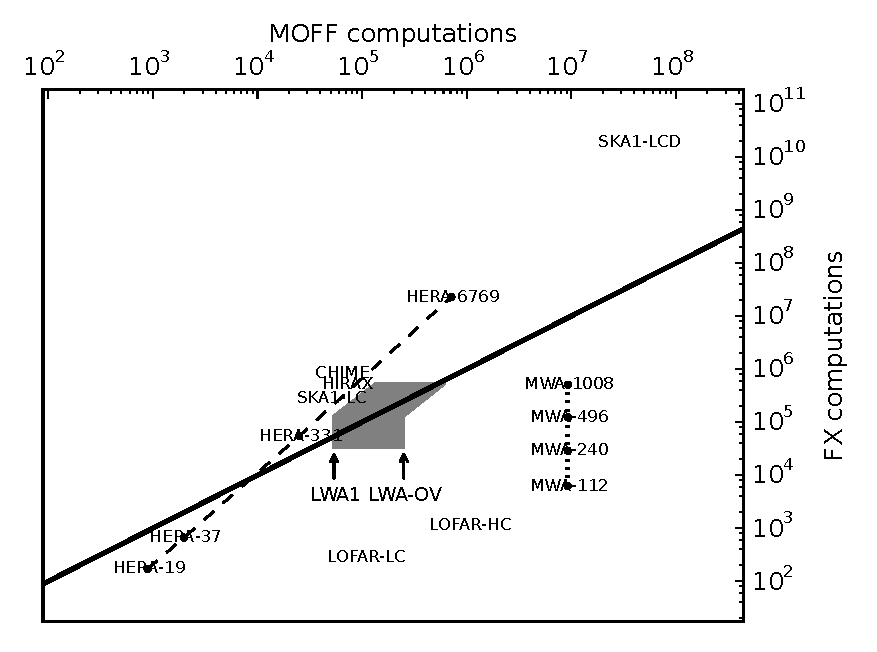
\includegraphics[width=\columnwidth]{figure11}
  % 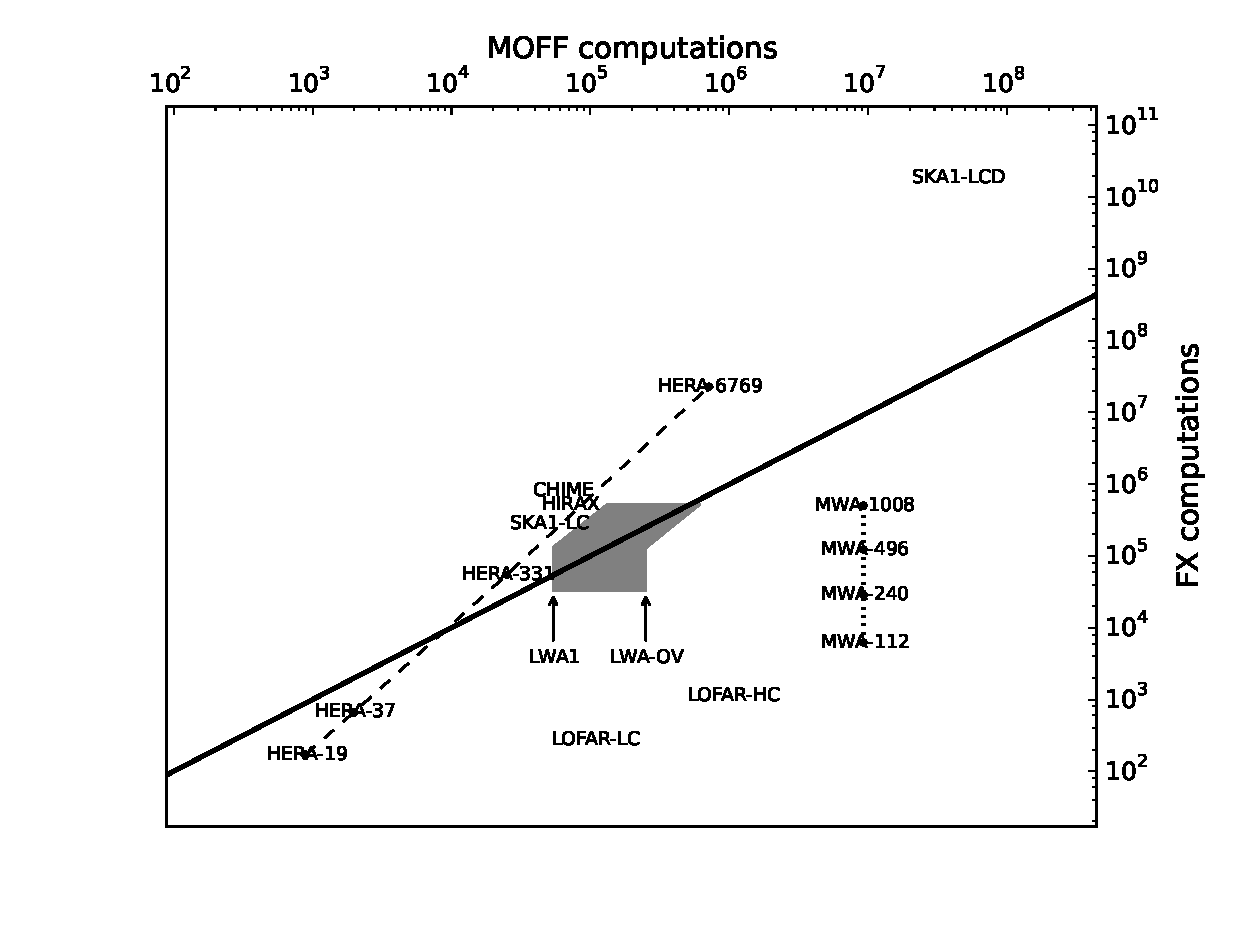
\includegraphics[width=\columnwidth]{MOFF_FX_computations_fov_gridding_annotated}
  % 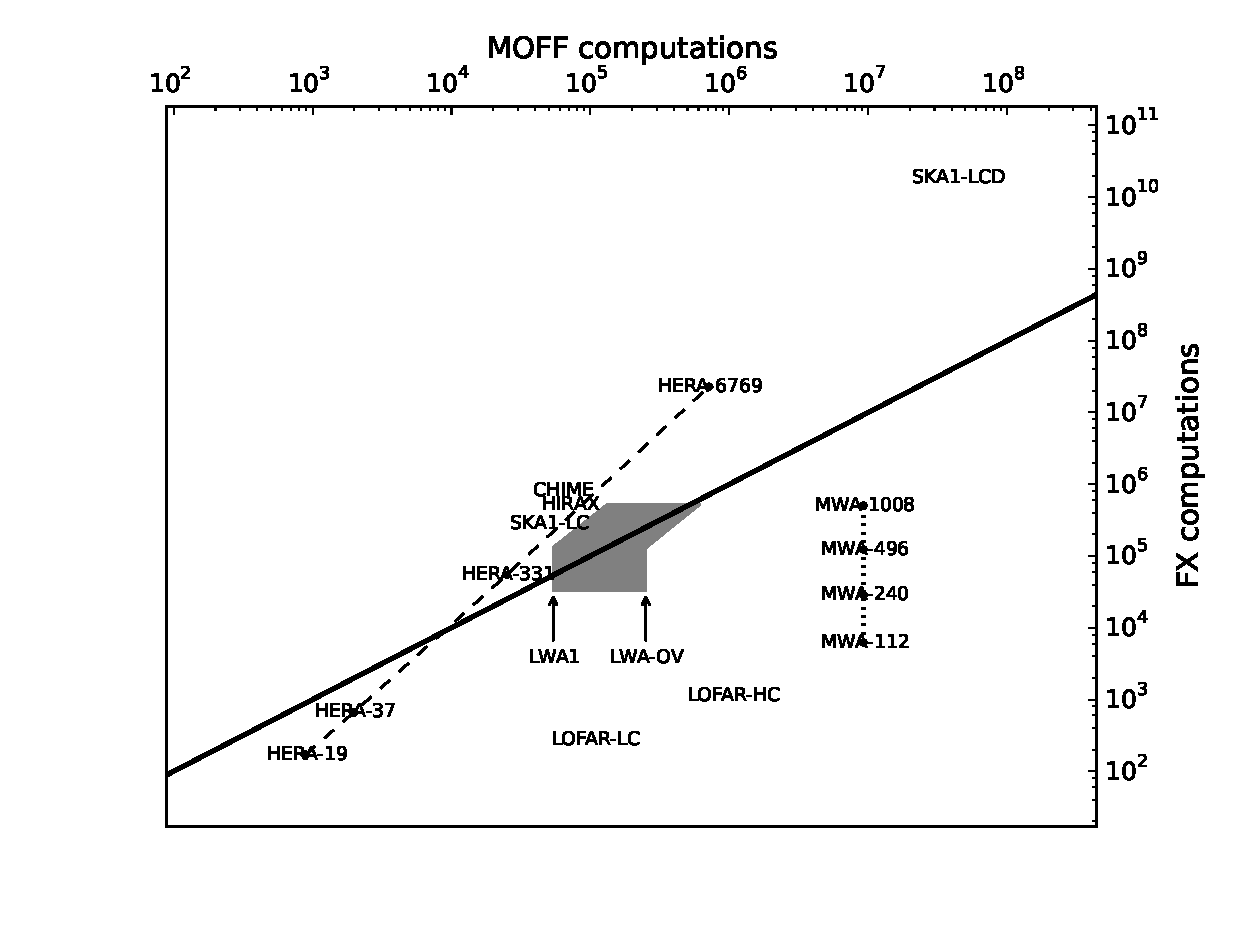
\includegraphics[width=\columnwidth]{MOFF_FX_computations_fov_gridding_annotated.eps}
  \caption{Current and planned instruments in parameter space of
    number of complex multiplies and adds with MOFF and FX. The solid line
    is the boundary at which the number of operations with MOFF and 
    visibility-based imaging are equal. MOFF imaging is more efficient for 
    telescopes occupying the left of this line and vice versa. CHIME, HIRAX, 
    SKA1-LC, SKA1-LCD and all the HERA layouts except HERA-19 and HERA-37 lie 
    in the parameter space favoured by MOFF imaging. The dashed line shows the 
    projected trajectory of hypothetical expanded HERA layouts. The dotted line 
    similarly shows hypothetical expanded MWA layouts with more tiles added in 
    the same core. The gray shaded area denotes the projected trajectory of the 
    LWA bounded by LWA1 (left edge), LWA-OV (right edge), current layout 
    (bottom) and a four-fold increase in the number of elements within a 50 per 
    cent increase in the core size (top). Current instruments such as MWA and 
    LOFAR fall in a region favoured by visibility-based imaging.}
  \label{fig:parameter-space-computations-instruments}
\end{figure}

We now consider antenna array layouts described by three essential quantities in radio interferometry, namely, maximum baseline length, number of antennas, and the size of each antenna. Fig.~\ref{fig:parameter-space-bll-nant-instruments} shows the boundaries where the ratio of the number of computations required with visibility-based imaging relative to MOFF imaging is unity. The different colored lines correspond to different antenna sizes (cyan - 1~m$^2$, blue - 7~m$^2$, purple - 16~m$^2$, green - 28~m$^2$, orange - 150~m$^2$, red - 740~m$^2$, gray - 5900~m$^2$). {\bf Dashed lines of each color denote the boundary to the left of which the MOFF algorithm is favoured for the corresponding antenna size and vice versa for visibility-based imaging.} 

\begin{figure}
  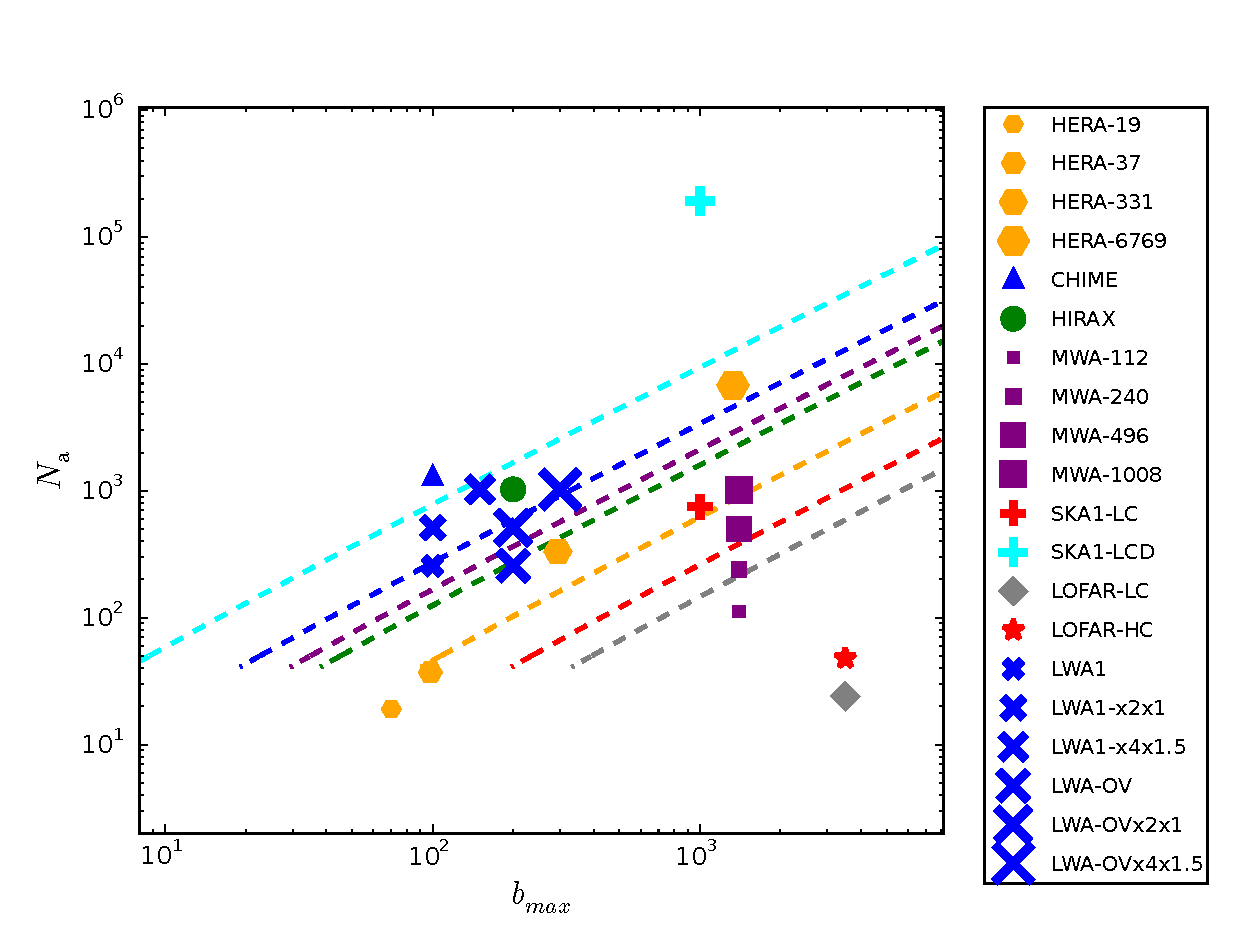
\includegraphics[width=\columnwidth]{figure12}
  % 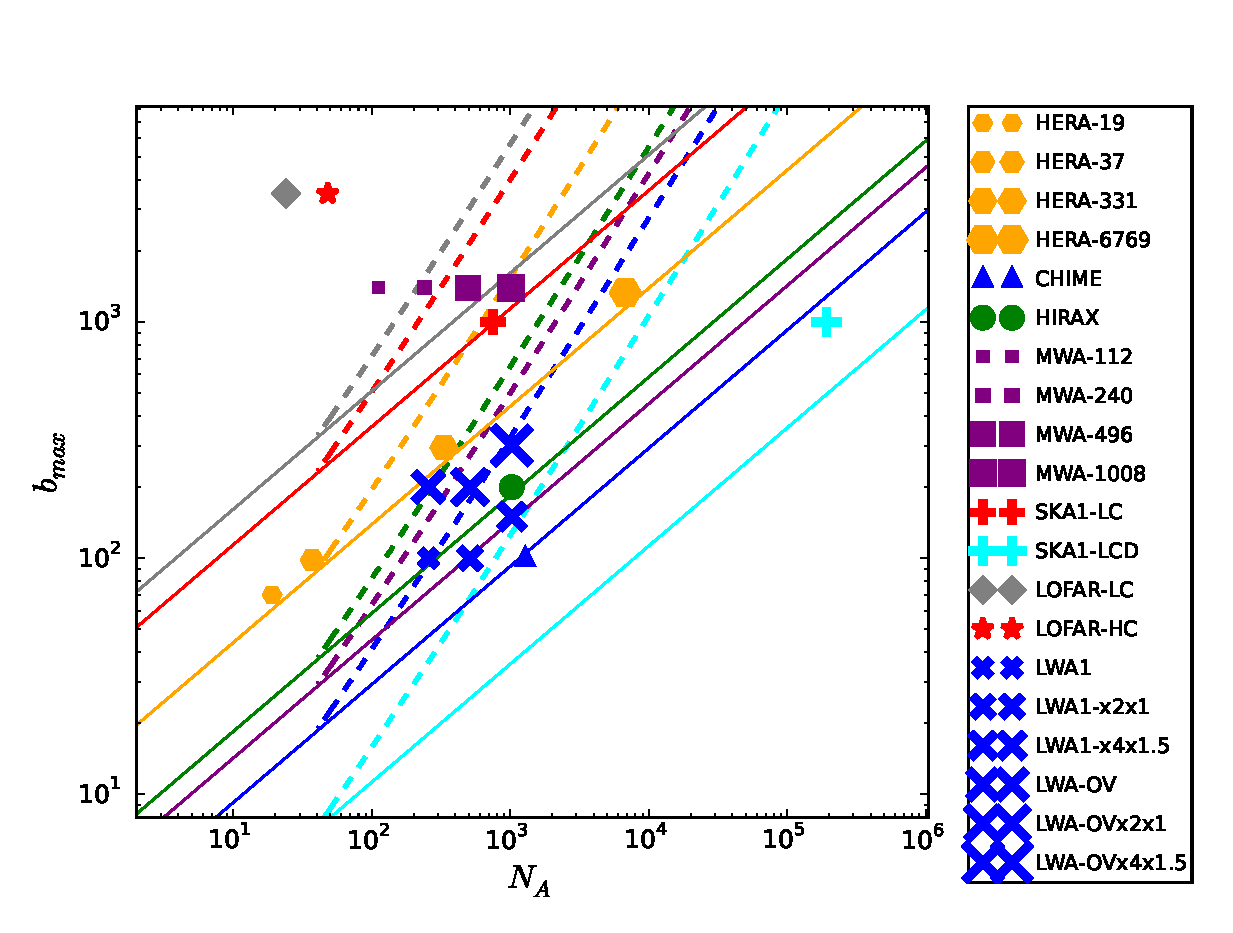
\includegraphics[width=\columnwidth]{MOFF_FX_crossover_baseline_n-antennas_rho_fov_gridding_legended}
  % 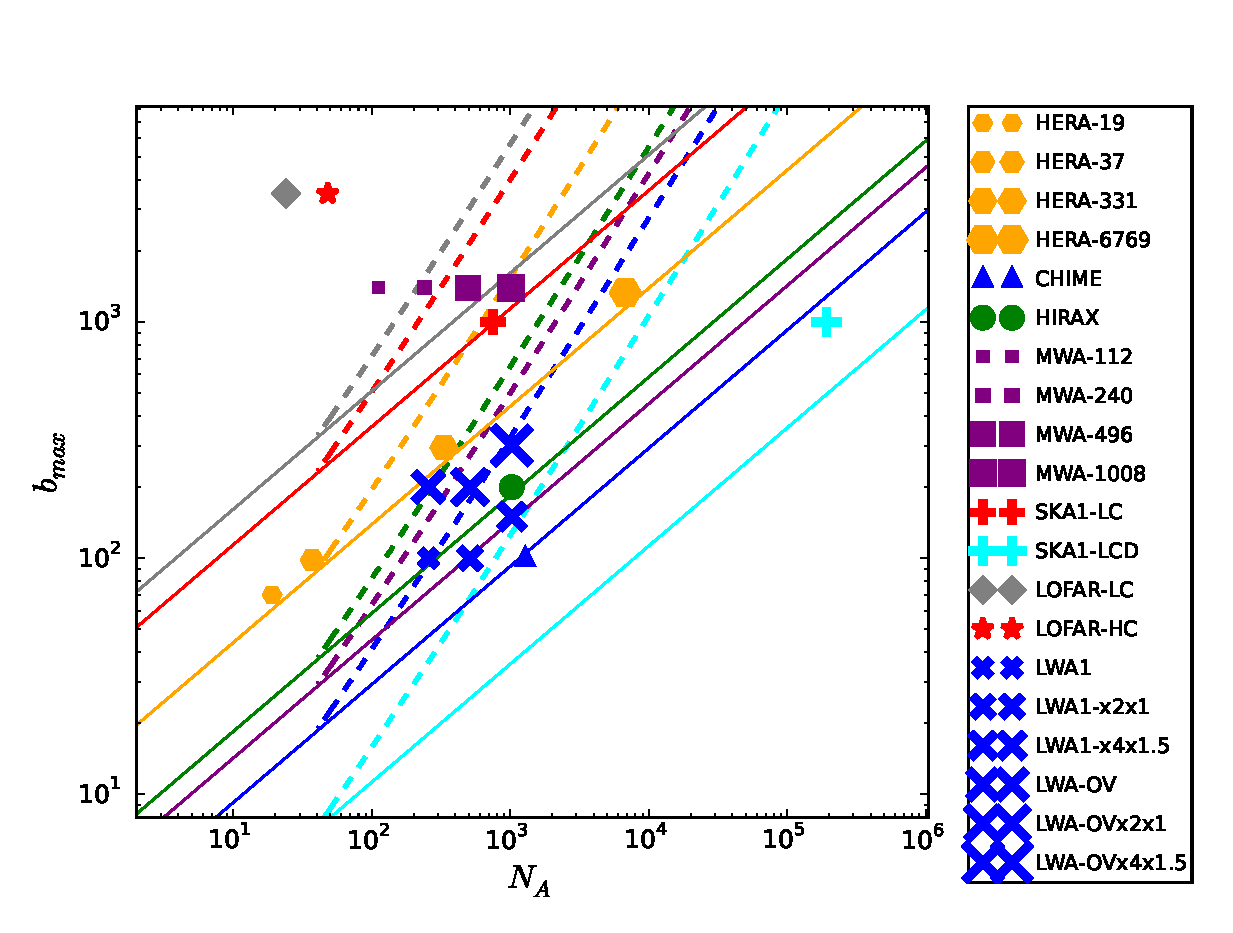
\includegraphics[width=\columnwidth]{MOFF_FX_crossover_baseline_n-antennas_rho_fov_gridding_legended.eps}
  \caption{Current and planned instruments in parameter space of baseline length and number of antennas with MOFF and FX. Lines of different colors denote different classes of antenna sizes (cyan - 1~m$^2$, blue - 7~m$^2$, purple - 16~m$^2$, green - 28~m$^2$, orange - 150~m$^2$, red - 740~m$^2$, gray - 5900~m$^2$). Lines of each color denote the boundary to the left of which MOFF algorithm is favoured for the corresponding antenna size. These lines shift rightward with increasing antenna size. The different antennas are color coded by roughly the class of antenna size they fall into. {\bf Thus symbols of one color falling to the left of a line} of the same color indicate MOFF imaging is advantageous for those telescopes and vice versa. For example, MOFF imaging is favoured in HERA-331 and HERA-6769 because they {\bf lie to the left of the orange line} but not so in cases of HERA-19 and HERA-37.}
  \label{fig:parameter-space-bll-nant-instruments}
\end{figure}

{\bf There is an upper limit set by the maximum number of antennas for each antenna size that can be densely packed inside various baseline lengths but is not shown on this figure to avoid crowding. We note that as antenna size increases the maximum number of antennas for a dense packing as a function of baseline length decreases. Hence, this upper limit shifts rightward as antenna size increases. Similarly, with increase in antenna size, $\Ngrid$ also decreases when field of view imaging is achieved with an increased grid spacing equal to antenna size and hence lowers the amount of computations required with the MOFF algorithm. This shifts the dashed lines rightward as well.}

{\bf The different antennas are color coded by roughly the class of antenna size they fall into. Thus symbols of one color that lie to the left of same colored line indicate MOFF imaging is favoured for those telescopes and vice versa. For e.g., MOFF imaging is favoured in HERA-331 and HERA-6769 because they lie to the left of the orange line but not so in cases of HERA-19 and HERA-37}. A majority of the next-generation radio telescopes, namely, HERA-331 and its future expanded versions, SKA1-LC, SKA1-LCD, HIRAX, and CHIME will fall in the regime where MOFF imaging will be desirable. LWA1 and LWA-OV are already very close to the dividing line. Their hypothetical expansions,\footnote{LWA1-x2x1 and LWA1-x4x1.5, and LWA-OVx2x1 and LWA-OVx4x1.5 denote two-fold and four-fold increase in number of antennas within a core diameter that is 1 and 1.5 times the current size of 100~m and 200~m respectively for LWA1 and LWA-OV.} will be in the computational regime favoured by MOFF. For a fixed baseline length, regions favouring the MOFF algorithm tend to be towards large $\Nant$ indicating large-N dense array layouts with smaller antenna elements are best suited for deploying EPIC.

\subsection{Data Throughput}

We elaborate on the I/O data rates required with the MOFF and visibility-based
algorithms. This is particularly relevant in the context of radio transient 
detection. 

Implementation of the MOFF algorithm with EPIC yields calibrated images on
time-scales of the output generated by the digitizer and is set by the inverse
of the frequency channel width. These calibrated images are accumulated and 
averaged to a certain time-scale depending on science or hardware requirements,
or when the sky has rotated significantly, whichever is lesser. In 
visibility-based algorithms, the visibilities are accumulated and averaged to 
this time-scale before images are produced. Thus the data throughput (in samples 
per second) per cross-polarization with MOFF and X-engine outputs are: 
\begin{align}
  r_\textrm{MOFF} &\sim \frac{4\Ngrid}{\Delta t} \left(\frac{\Delta B}{\Delta f}\right) \\
  r_\textrm{X} &\sim 2\,\frac{\Nant(\Nant-1)/2}{\Delta t} \left(\frac{\Delta B}{\Delta f}\right),
\end{align}
where, the factor 4 in the expression for $r_\textrm{MOFF}$ accounts for imaging
after zero-padding the gridded electric fields, the leading factor of 2 in the
expression for $r_\textrm{X}$ accounts for the real and imaginary parts of the
complex visibilities, $\Delta B$ is the bandwidth, $\Delta f$ is the frequency 
resolution, and $\Delta t$ is the time-scale over which the transient phenomenon
is sampled and the data (images or visibilities) are averaged to.

Though a full understanding of the FRB phenomena is yet to emerge, there are 
indications the time-scales of FRB objects are $\Delta t \sim 1$--10~ms 
\citep{tho13}. For a telescope like HERA, $\Delta B \simeq 100$~MHz, 
$\Delta f \simeq 100$~kHz. For HERA-331, $\Nant=331$ and with a grid 
spacing to image the field of view, $\Ngrid \simeq 441$ or 
$\Ngrid \simeq 1024$ if $\Ngrid$ is preferred as a power of 2 in either 
direction. Using 8 bytes for each floating point sample in the MOFF images and 
4 bytes each for real and imaginary parts of visibility samples, the throughputs 
are $r_\textrm{MOFF} \lesssim 3$~GB~s$^{-1}$ and 
$r_\textrm{X} \simeq 41$~GB~s$^{-1}$. For HERA-37, 
$r_\textrm{MOFF} \lesssim 190$~MB~s$^{-1}$ and 
$r_\textrm{X} \simeq 0.5$~GB~s$^{-1}$. In such a case, The X-engine throughput 
corresponds to an extreme rate of $\simeq 1.8$~TB an hour per 
cross-polarization. Conversely, for the same data throughput, the MOFF algorithm 
can sample even shorter time-scales. 

Table~\ref{tab:data-rates} shows these data rates for some of the current and 
planned telescopes for $\Delta t=10$~ms. In almost all cases listed, even with 
conservative estimates, the MOFF algorithm provides very economic data 
throughput for a majority of next generation radio telescopes with a dense 
layout. The most significant advantage is that calibrated images are also 
available at no extra cost.

\begin{table}
  \centering
  \caption{Data throughput per cross-polarization for various telescopes with 
    MOFF and X-engine outputs on time-scales of $\Delta t=10$~ms assuming 
    $\Delta B=100$~MHz and $\Delta f=100$~kHz.}
  \label{tab:data-rates}
  \begin{threeparttable}
  \begin{tabular}{ccc} 
    \hline
    Telescope\tnote{a} & $r_\textrm{MOFF}$\tnote{b} & $r_\textrm{X}$ \\
              & (GB~s$^{-1}$)\tnote{c} & (GB~s$^{-1}$)\tnote{c} \\
    \hline
    LWA1 & $\simeq 3$ & $\simeq 24.3$ \\
    LWA-OV & $\simeq 12$ & $\simeq 24.3$ \\
    HERA-19 & $\lesssim 0.19$ & $\simeq 0.13$ \\
    HERA-37 & $\lesssim 0.19$ & $\simeq 0.5$ \\
    HERA-331 & $\lesssim 3$ & $\simeq 41$ \\
    CHIME & $\lesssim 6.1$ & $\simeq 610$ \\
    \hline
  \end{tabular}
  \begin{tablenotes}
    \item[a] Antenna layouts are listed in Table~\ref{tab:antenna-layouts}.
    \item[b] $\Ngrid$ is usually greater than true value because of 
      rounding to the next power of 2 in either direction. Thus 
      $r_\textrm{MOFF}$ is usually lesser than the conservative values 
      listed here.
    \item[c] We assume 8 bytes for each real sample from MOFF images, and
      4 bytes each for real and imaginary parts of visibility samples.
  \end{tablenotes}
  \end{threeparttable}
\end{table}

\section{Conclusions}\label{sec:conclusions}

As radio astronomy is entering a new era, advances in instrumentation have to be accompanied by equal advances in processing techniques to manage computational resources. Many future radio telescopes such as the SKA, HERA and LWA are headed towards the large-N dense array layout model for which computational cost from traditional FX/XF correlator-based architecture and visibility-based imaging starts rising steeply. We have provided the first software demonstration of a general purpose imaging algorithm using our generic and efficient EPIC software that is designed to bring this cost down from $\mathcal{O}(\Nant^2)$ to $\mathcal{O}(\Ngrid\log_2 \Ngrid)$. Under the class of direct imaging techniques, ours is one of the most generic -- neither does it place any constraint on the array layout to be on a regular grid nor does it require the antenna array to be homogeneous. {\bf We have demonstrated its natural ability to robustly image data from heterogeneous arrays and shown that wrong assumptions about array homogeneity could result in significant and systematic mis-estimation of the sky model.}

Our EPIC package, now publicly available, written in object oriented Python, is 
highly modularized and parallelizable. It includes an implementation of the 
MOFF algorithm in addition to visibility-based software holography imaging and 
a data simulator for sky models. It is designed to provide a development 
platform to compare different imaging approaches and serve as a stepping stone 
for real-life GPU/FPGA-based implementation on telescopes. It has been 
successfully tested on simulated MWA observations as well as real LWA 
observations {\bf from both imaging and calibration view points}. 

The MOFF algorithm packaged with EPIC is already found to be most suitable 
for many present and planned radio telescopes such as the LWA, HERA, CHIME,
HIRAX and SKA. In general, MOFF is most suited to operate in the region of 
parameter space characterized by dense packing of a large number of antennas 
especially when consisting of a large number of small antenna elements. 

It is seen to have significant savings in data throughput relative to a 
X-engine based pipeline. A unique advantage is the instantaneous availability 
of calibrated time-domain images at no extra cost. Hence, it is a compelling 
candidate for time-domain radio astronomy, e.g. search for and monitoring of 
transients. Potentially, it could allow on-chip processing thus lowering even 
further the already relatively low I/O bandwidth shown in 
Table~\ref{tab:data-rates} except when a transient event is detected. Transient 
detection pipelines at the backend of EPIC can be fine-tuned to target fast 
transients such as the Fast Radio Bursts \citep[FRB;][]{tho13} on millisecond 
time-scales at GHz frequencies or slow transients from planetary and exoplanetary 
origins at frequencies around 100~MHz. 

Thus, EPIC with the MOFF algorithm packaged is uniquely poised to offer a
substantial advantage to imaging with large-N dense arrays typical of 
next-generation radio telescopes as well as push the frontiers of 
time-domain astronomy to fill gaps in understanding the science behind 
phenomena responsible for extreme transient events in the Universe.

In the near future, we plan to {\bf demonstrate speed and precision by upgrading EPIC to a GPU-based implementation} in order to operate on real-time data and develop a transient trigger and monitor backend. {\bf In the meanwhile, we plan to demonstrate imaging with non-coplanar arrays and direction-dependent calibration.} 

\section*{Acknowledgements}

We thank Larry D'Addario, Gregg Hallinan, Joseph Lazio and Harish Vedantham for 
their valuable inputs, and Greg Taylor for providing us with LWA data. This work 
has been supported by the National Science Foundation through award AST-1206552. 
Construction of the LWA has been supported by the Office of Naval Research under 
Contract N00014-07-C-0147. Support for operations and continuing development of 
the LWA1 is provided by the National Science Foundation under grant AST-1139974 
of the University Radio Observatory program.

%%%%%%%%%%%%%%%%%%%% REFERENCES %%%%%%%%%%%%%%%%%%

\bibliographystyle{mnras}
\bibliography{epic} 
% \bibliography{../epic} 
% 
% Basic setup. Most papers should leave these options alone.
\documentclass[a4paper,fleqn,usenatbib]{../mnras}

\usepackage{newtxtext,newtxmath}

% Use vector fonts, so it zooms properly in on-screen viewing software
% Don't change these lines unless you know what you are doing
\usepackage[T1]{fontenc}
\usepackage{ae,aecompl}


%%%%% PACKAGES %%%%%

% Only include extra packages if you really need them. Common packages are:
\usepackage{graphicx}	% Including figure files
\usepackage{amsmath}	% Advanced maths commands
\usepackage{amssymb}	% Extra maths symbols
\usepackage{color}

%%%%% CUSTOM COMMANDS %%%%%

\newcommand{\Nant}{\ensuremath{N_{\mathrm{a}}}}
\newcommand{\Ng}{\ensuremath{N_{\mathrm{g}}}}
\newcommand{\s}{\ensuremath{\hat{\mathbf{s}}}} % s-hat for sine-projected direction
\newcommand{\spix}{\ensuremath{\hat{\mathbf{s}}_{0}}}
\newcommand{\Cna}[1][n]{\ensuremath{\mathcal{C}^{(#1)}_{a,\spix}}}
\newcommand{\ri}{\ensuremath{\mathbf{r}_i}}
\newcommand{\ra}{\ensuremath{\mathbf{r}_a}}
\newcommand{\rb}{\ensuremath{\mathbf{r}_b}}
\newcommand{\beamr}{\ensuremath{\widetilde{W}}}
\newcommand{\beamtheta}{\ensuremath{W}}
\newcommand{\Er}[1]{\ensuremath{\widetilde{E}_{#1}}}
\newcommand{\Erest}[1]{\ensuremath{\widetilde{E}'_{#1}}}
\newcommand{\Ethetaest}{\ensuremath{E'}}
\newcommand{\V}{\ensuremath{\widetilde{V}}}
\newcommand{\dif}{\mathrm{d}}
\newcommand{\caliter}{400}
\newcommand{\damp}{\ensuremath{\gamma}}
\newcommand{\itr}{20}

%%%%%%%%%%%%%%%%%%% TITLE PAGE %%%%%%%%%%%%%%%%%%%

% Title of the paper, and the short title which is used in the headers.
% Keep the title short and informative.
\title[E-field Parallel Imaging Calibration]{An Efficient E-field Parallel Imaging Calibration Algorithm for Next-Generation Radio Telescopes}

% The list of authors, and the short list which is used in the headers.
% If you need two or more lines of authors, add an extra line using \newauthor
\author[Beardsley et al.]{
Adam P. Beardsley,$^{1}$\thanks{E-mail: Adam.Beardsley@asu.edu}
Nithyanandan Thyagarajan,$^{1}$
Judd D. Bowman$^{1}$
\newauthor
and Miguel F. Morales$^{2}$
\\
% List of institutions
$^{1}$Arizona State University, School of Earth and Space Exploration, Tempe, AZ 85287, USA\\
$^{2}$University of Washington, Department of Physics, Seattle, WA 98195, USA\\
}

% These dates will be filled out by the publisher
\date{Accepted XXX. Received YYY; in original form ZZZ}

% Enter the current year, for the copyright statements etc.
\pubyear{2015}

% Don't change these lines
\begin{document}
\label{firstpage}
\pagerange{\pageref{firstpage}--\pageref{lastpage}}
\maketitle

% Abstract of the paper
\begin{abstract}
Abstract here (250 words)
\end{abstract}

\begin{keywords}
instrumentation: interferometers -- techniques: image processing -- techniques: interferometric
\end{keywords}


%%%%%%%%%%%%%%%%% BODY OF PAPER %%%%%%%%%%%%%%%%%%

\section{Introduction}
In order to satisfy the survey speeds required for precision cosmology as well as searches for fast radio transients, radio astronomy is undergoing a paradigm shift toward interferometers consisting of hundreds to thousands of small, widefield antennas. Many arrays with this design are already built or under construction including the Hydrogen Epoch of Reionization Array\footnote{http://reionization.org} (HERA), the Murchison Widefield Array (MWA;\citealt{tin13,bow13}), the Precision Array for Probing the Epoch of Reionization (PAPER; \citealt{par10}), the LOw Frequency ARray (LOFAR; \citealt{van13}), the Canadian Hydrogen Intensity Mapping Experiment (CHIME,\citealt{ban14}), the Long Wavelength Array (LWA, \citealt{ell13}), and the low frequency Square Kilometer Array (SKA1-Low \citealt{mel13}).

Traditional radio correlators cross-multiply the voltage signals from all pairs of antennas, and the computation scales as the number of antennas squared, $\mathcal{O}(\Nant^2)$ \citep{bun04}. As the number of elements in future arrays grows, the computational cost will become prohibitively expensive, and exploring efficient correlator schemes is essential to enable next generation instruments \citep{lon00}. Meanwhile, radio transient monitoring requires access to high time and frequency resolution data. For example, fast radio bursts (FRBs) are highly unexplored at low frequencies (< 1 GHz), but are expected to occur on timescales $\Delta t \sim$ 1--10~ms \citep{tho13}. Recording the full visibility matrix for $\Nant \gtrsim 10^3$ arrays at this timescale leads to extremely high data write rates. 

Direct imaging correlators are a new variety of radio correlator which aim to alleviate both the computational strain of forming $\Nant^2$ correlations and the high data throughput associated with short timescale science. This is done by performing a spatial fast Fourier transform (FFT) to image the antenna voltages, then squaring and averaging in time. This process scales as $\mathcal{O}(\Ng \log_2 \Ng)$, where \Ng~is the number of grid points in the FFT \citep{mor11, teg09, teg10}. For certain classes of telescopes, significantly those envisioned for next generation cosmology experiments, this scaling is a large improvement over the $\Nant^2$ scaling of traditional methods. Furthermore, because images are generated online, the native output bandwidth will be lowered (assuming $\Ng < \Nant^2$), and has the potential to be lowered even further with online transient processing.

A handful of prototype direct imaging correlators have been tested on arrays including the Basic Element for SKA Training II (BEST-2) array \citep{fos14}, the Omniscope \citep{zhe14}, and an earlier pulsar timing experiment at GHz frequencies \citep{oto94, dai00}. Each of these are examples of so-called FFT correlators -- a subclass of direct imaging correlators which rely on identical antennas with restricted placement, which allows the FFT to be performed without gridding. We recently released the E-field Parallel Imaging Correlator \citep[EPIC;][]{thy15c}, which is a software implementation of the Modular Optimal Frequency Fourier \citep[MOFF;][]{mor11} imaging algorithm. This architecture leverages the software holography/A-transpose framework to grid electric field data streams before performing the spatial FFT, allowing for an optimal map without placing constraints on array layout or requiring identical antennas \citep{mor09,bha08,teg97a}.

A challenge common to all direct imaging algorithms is calibration of the antenna gains. Traditionally, pair-wise visibilities are written to disk and used to calibrate offline. However, a direct imaging correlator mixes the signals from all antennas before averaging and writing to disk, making calibration a requirement at the front end. Previous solutions have involved applying calibration solutions generated from a parallel FX correlator \citep{zhe14, fos14}, or integrating a dedicated FX correlator which periodically formed the full visibility matrix to solve for gains \citep{wij09,dev09}. While these solutions were sufficient to enable the exploration of FFT correlators and beamformers, they will not scale to future arrays with $\Nant \gtrsim 10^3$.

Here we present the E-field Parallel Imaging Calibration (EPICal) algorithm -- a novel solution to the calibration problem, which can be integrated into direct imaging correlators and scales only as the number of antennas, $\mathcal{O}(\Nant)$. This method uses a correlation of the uncalibrated antenna signal stream with an output image pixel from the backend of the correlator to solve for the complex gains of the antennas. Because the calibration must be applied before gridding and imaging, our solution requires an iterative approach where the data from one time series is used to update the gains which are applied to the following time series. An example implementation of the algorithm is available with the EPIC software package\footnote{http://github.com/nithyanandan/EPIC}.

We establish the mathematical framework and derive the calibration algorithm in \S \ref{sec:math}. We then demonstrate the algorithm in simulations in \S \ref{sec:sim}, and apply to a sample LWA data set in \S \ref{sec:data}. Then we discuss the noise properties of the resulting gain solutions in \S \ref{sec:noise}. Finally we conclude and discuss potential extensions to the algorithm in \S \ref{sec:discussion}.

\section{Mathematical Framework}\label{sec:math}
We begin by establishing the mathematical framework for the calibration problem. We derive the calibration solutions for the MOFF algorithm (adopting the notation of \citealt{thy15c}), but note the result is easily extended to FFT correlator algorithms by removing the gridding step.

The electric field incident on the ground, $\Er{}(\mathbf{r},f,t)$, is related to the sky electric field, $E(\hat{\mathbf{s}},f,t)$, through a Fourier transform.
\begin{equation}
\Er{}(\mathbf{r},f,t) = \int E(\hat{\mathbf{s}},f,t) e^{-2\pi i \mathbf{r}\cdot \hat{\mathbf{s}}}\, \dif^2 \hat{\mathbf{s}}
\end{equation}
Here $\hat{\mathbf{s}}$ denotes the sine-projected unit vector for the sky angle, $\mathbf{r}$ is the observer's location (measured in wavelengths relative to an arbitrary origin), and $f$ and $t$ denote the frequency and time dependence, respectively. We will encounter several quantities which we attempt to estimate. We distinguish the ``true" values with a superscript $T$, while the estimates are denoted with a prime. We define the true antenna signal as a convolution of the antenna voltage pattern, $\beamr$, with the electric field on the ground.
\begin{equation}
\Er{a}^T(f,t) \equiv \int \beamr_a(\mathbf{r}-\ra) \Er{}(\mathbf{r},f,t) \, \dif^2 \mathbf{r}
\end{equation}
The subscript $a$ labels the antenna, and $\mathbf{r}_a$ is the location of antenna $a$.

We next model the measured, uncalibrated electric field as a multiplicative complex gain and an additive noise term applied to the true antenna electric field. 
\begin{equation}\label{eq:apply_gain}
\Er{a}(f,t) = g^T_a(f,t) \Er{a}^T(f,t) + \widetilde{n}_a(f,t)
\end{equation}
Note that this quantity is neither a true or estimated value. The noise term is strictly receiver noise -- noise introduced by the instrument. Any sky noise is implicitly included in the time dependence of the sky electric field. As the noise of modern low frequency arrays is heavily dominated by sky noise, we will neglect $\widetilde{n}_a$ for now, but will inspect its effects at the end of this section.

The goal of our calibration algorithm will be to estimate the antenna gains. We will assume the gains have no time dependence within the timescale of finding our solutions. \textcolor{red}{cite someone about gain stability}. Furthermore, we will treat each frequency channel independently, and drop the $f$ to simplify notation.

The MOFF algorithm next calls for a calibration. We will assume we have formed an estimate of the gains after $n$ iterations of a calibration loop, and derive an updated $n+1$ estimate. Typically calibration amounts to dividing the measured fields by the gain (in the case of sky noise dominance), or multiplying by the complex conjugate of the gain (receiver noise dominance). We will abstain from this choice for now, and instead use a multiplicative factor $h^{(n)}_a$ to represent the application of our $n^{\mathrm{th}}$-loop estimate of the gain for antenna $a$:
\begin{equation}
\Erest{a} = h^{(n)}_a \Er{a}
\end{equation}
where,
\begin{equation}
h^{(n)}_a=\begin{cases}
1/g^{(n)}_a & \mbox{sky noise dominated} \\ 
g^{*(n)}_a & \mbox{receiver noise dominated}.
\end{cases}
\end{equation}

A dirty image is next formed by gridding the calibrated fields with the antenna voltage pattern, Fourier transforming, squaring, and averaging in time. The estimated value for a pixel, $\s_i$, can be expressed as
\begin{equation}
I'(\s_i) = \left<\left| \frac{1}{\Nant}\sum_i e^{2\pi i \mathbf{r}\cdot \s_i} \sum_a \beamr_a(\ri - \ra) h^{(n)}_a g^T_a \Er{a}^T(t) \right|^2 \right>_t.
\end{equation}
This is the final output of the MOFF correlator. However, for calibration purposes we will be interested in the electric field image just prior to squaring and averaging.
\begin{equation}
\Ethetaest (\s_i,t) = \frac{1}{\Nant} \sum_i e^{2\pi i \ri \cdot \s_i} \sum_a \beamr_a(\ri - \ra) h^{(n)}_a g^T_a \Er{a}^T(t)
\end{equation}
We can simplify this expression by exchanging the sums to transform the beam term into sky coordinates.
\begin{align}\label{eq:epix}
\Ethetaest(\s_i,t) & = \frac{1}{\Nant} \sum_a h^{(n)}_a g^T_a\Er{a}^T(t) e^{2\pi i \s_i \cdot \ra}\sum_i \beamr_b(\ri-\ra)e^{2\pi i \s_i \cdot (\ri-\ra)} \nonumber\\
& = \frac{1}{\Nant} \sum_a h^{(n)}_a g^T_a\Er{a}^T(t) e^{2\pi i \s_i \cdot \ra}\beamtheta_a(\s_i)
\end{align}

Next we move toward the feedback calibration outlined in \citealt{mor11}. The calibration loop described there assumed a simple sky of a single point source, but we aim for a more generalized solution for arbitrarily complex sky models. As such the quantity we wish to inspect is a correlation of the uncalibrated antenna signals input to the correlator with the holographic electric field image output from the correlator. We define the quantity,
\begin{equation}\label{eq:Cna}
\Cna \equiv \left<\Er{a}(t) E'^*(\spix,t)\right>_t,
\end{equation}
where the superscript $n$ again represents the quantity formed in the $n^\mathrm{th}$ calibration loop, and \spix\, is the pixel center nearest a bright calibrator of interest. The following will hold for any chosen pixel, \spix, though it is advantageous to choose a pixel which contains a bright source to achieve a high signal to noise. 

Plugging equation \ref{eq:epix} into equation \ref{eq:Cna}, we find,
\begin{align}\label{eq:cna}
\Cna & = \left<g^T_a \Er{a}^T(t) \frac{1}{\Nant} \sum_b h^{*(n)}_b g^{T*}_b\Er{b}^{T*}(t) e^{-2\pi i \spix \cdot \rb} \beamtheta^*_b(\spix)\right>_t \nonumber \\
& = \frac{g^T_a}{\Nant} \sum_b h^{*(n)}_b g^{T*}_b \beamtheta^*_b(\spix) e^{-2\pi i \spix \cdot \rb} \left<\Er{a}^T \Er{b}^{*T} \right>_t \nonumber \\
& = \frac{g^T_a}{\Nant} \sum_b h^{*(n)}_b g^{T*}_b \beamtheta^*_b(\spix) e^{-2\pi i \spix \cdot \rb} \V^T_{ab}
\end{align}
where in the second step we group time-dependent terms, and in the third we define the true visibilities as the correlation between true antenna electric field measurements. It is easy to see from here that the net effect of including the receiver noise term, $\widetilde{n}_a(f,t)$, will result in added noise on the true visibilities. In principle this can include any noise correlations between antennas. The implementation included in the EPIC software package restricts the noise term to include only the auto-correlation noise bias, and assumes baseline dependent noise is zero mean.

Finally, we find an update to our gain solution by assuming our current estimate of the gains, $g^{(n)}_b$, is approximately correct and substitute into the sum for the true gains. We also require model visibilities formed from sky and primary beam models in place of true visibilities.
\begin{equation}\label{eq:cal_solution}
g'^{(n+1)}_a = \Cna \Nant \left[ \sum_b h^{*(n)}_b g^{*(n)}_b \beamtheta^*_b(\spix) e^{-2\pi i \spix \cdot \rb} \V^T_{ab} \right]^{-1}
\end{equation}
This equation is our prescription for estimating the antenna gains of a direct imaging array. The approach is iterative in nature, and requires a sky model. However, the sky model can be precomputed offline, and the online computation complexity scales only as $\mathcal{O}(\Nant)$ as we form a $\Cna$ for each antenna. In the case where $h_b = 1/g_b$ (typical calibration procedure for sky-noise dominated systems), this simplifies slightly.
\begin{equation}\label{eq:cal_solution_simple}
g'^{(n+1)}_a = \Cna \Nant \left[ \sum_b \beamtheta^*_b(\spix) e^{-2\pi i \spix \cdot \rb} \V^T_{ab} \right]^{-1}
\end{equation}

While testing we found equation~\ref{eq:cal_solution} resulted in oscillatory gain solutions as it was iterated, as is often the case in iterative minimization methods. To mitigate this we introduce a damping factor, $0 \leq \damp <1$, which is used to attenuate the gain update, effectively giving the solutions memory of previous iterations.
\begin{equation}
g^{(n+1)}_a = (1-\damp) g'^{(n+1)}_a + \damp g^{(n)}_a
\end{equation}
We found that while equation~\ref{eq:cal_solution} does indeed converge on good solutions, the process is faster by tuning the damping factor. We note the small difference between $g^{(n+1)}_a$ and $g'^{(n+1)}_a$, where the prime indicates our current best estimate of the true gain, while no prime is actually used in the iterative calibration loop. Once the loop converges the difference is a longer effective integration for the non-primed version (lower thermal noise). 

We show schematically the process of calibrating a direct imaging correlator in figure~\ref{fig:schematic}. Computationally expensive steps that must be performed ``on-chip" are shown inside the gray box. The uncalibrated antenna signals are tapped out after the F-engine and correlated against the output image pixel of interest. The correlated values are then passed off-chip to estimate the gains using equation~\ref{eq:cal_solution}, and additional fitting if desired. The gains are then passed back to the correlator to update the calibration for subsequent data streams. 

\begin{figure}
\begin{center}
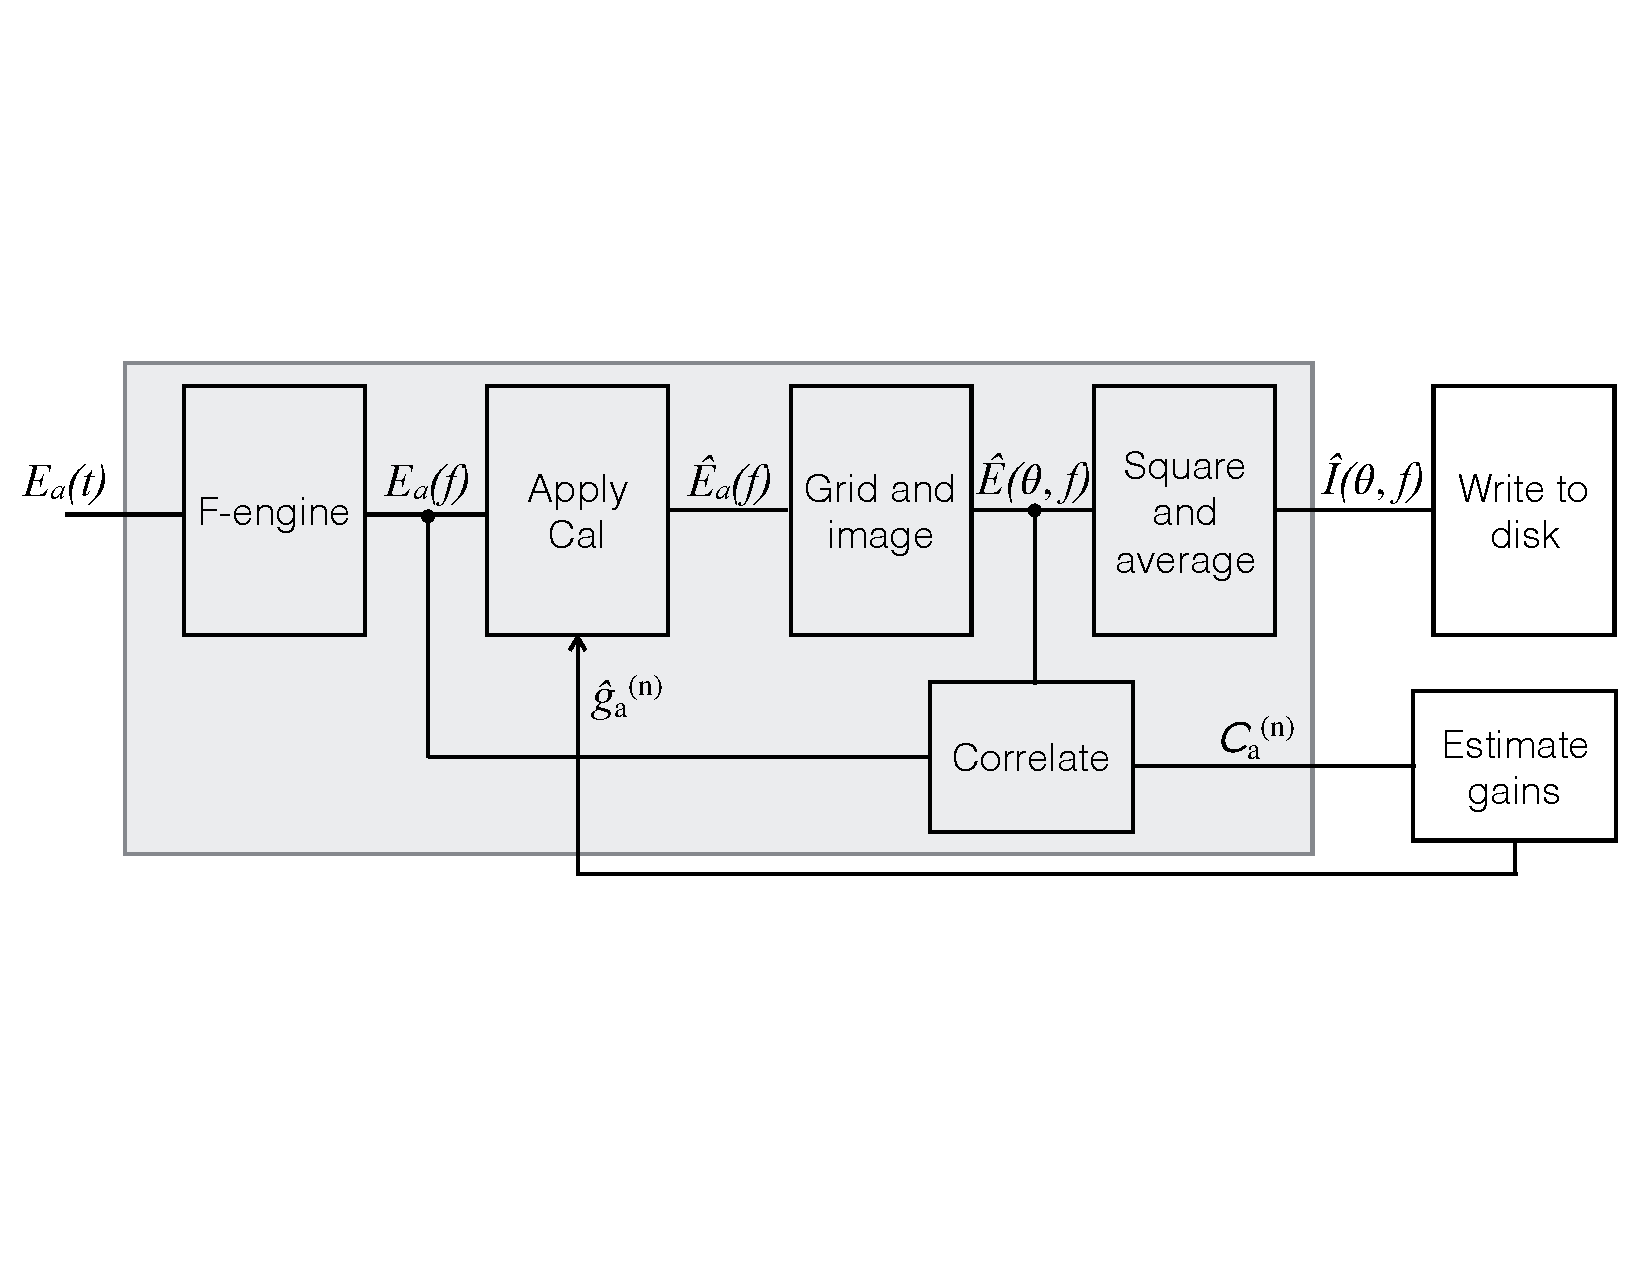
\includegraphics[width=\columnwidth]{figures/schematic.pdf}
\caption{The general data flow of the MOFF correlator, with a feedback calibration loop. A pixel from the (unsquared) image is tapped out and correlated against the input antenna electric field signals to form $\Cna$ coefficients, which are used to estimate the antenna gains. These gain estimates are then fed back into the correlator to be applied to subsequent data, and the process is repeated. The gray box shows operations which must be done at high speed (before averaging in time), which white boxes show operations which can be performed ``off-chip".}
\label{fig:schematic}
\end{center}
\end{figure}

An important feature to note is that, like the MOFF-generated images themselves, equations~\ref{eq:cal_solution} and~\ref{eq:cal_solution_simple} include the antenna auto-correlations (the sum is over \emph{all} $b$, not excluding $a$). It can be difficult to perfectly model the noise bias from auto-correlations, which can often times be far brighter than the visibilities themselves. It can therefore be beneficial to subtract this term directly from \Cna, and exclude the $b=a$ term in the sum.
\begin{equation}
\Cna \rightarrow \Cna - \frac{1}{\Nant} h^{*(n)}_a\beamtheta^*_a e^{-2\pi i \spix \cdot \ra} \left<|\Er{a}|^2\right>_t
\end{equation}
This requires generating these correlations, which again only scale as $\mathcal{O}(\Nant)$, and are generally useful for array diagnostics.

We conclude this section by connecting our calibration expression to that found in a visibility framework. In the limit of a single bright calibrating source at phase center, we can greatly simplify equations~\ref{eq:cna} and~\ref{eq:cal_solution}. We will assume the beams are normalized such that $\beamtheta(0)=1$. We can further drop the exponential phase terms because $\spix=0$. We then absorb the true gains and gain corrections into the true visibilities in equation~\ref{eq:cna} to express as a sum of measured visibilities.
\begin{equation}
\mathcal{C}^{(n)}_{a,0} \rightarrow \frac{1}{\Nant}\sum_b h^{*(n)}_b \V_{ab}
\end{equation}

We next plug this expression into equation~\ref{eq:cal_solution} to find our simplified calibration solution for a single bright point source. Because our sky is a single bright point source, the model visibilities are simply the flux of the source, $S_{\mathrm{src}}$.
\begin{equation}
g'^{(n+1)}_a \rightarrow \left[\sum_b h^{*(n)}_b \V_{ab}\right] \times \left[S_{\mathrm{src}}\sum_b h^{*(n)}_b g^{*(n)}_b\right]^{-1}
\end{equation}
This is simply a gain-weighted sum of the measured visibilities over the flux of the source, which is indeed the limiting result from a visibility approach, for example seen in \citealt{mit08}. The ability to recover the equivalent expression despite not actually forming the visibilities is a result of the fact that only sums over visibilities come into the FX solution, as was described in \citealt{mor11}. We have confirmed the limiting case equivalence here, and will explore the more general case in more detail in \S~\ref{sec:noise}.


\section{Simulation}\label{sec:sim}
We first demonstrate our calibration method through a controlled simulation. A complex gain is created for each antenna with random phase and amplitude, which is used to corrupt the simulated data stream, then we attempt to recover the gains using our calibration routine. The simulation software used is included in the EPIC package.

Our simulated signal consists of 10 random point sources with flux densities 0.5~Jy~$\lesssim S \lesssim 1$~Jy. For an antenna array we use the inner 51 antennas of the MWA layout \citep{bea12}, within a bounding box of 150~m. The antenna voltage pattern used is a 4.4~m square tophat on the ground. Because our algorithm treats frequency channels independently, we simulate only one channel. For context we treat this channel as a single 40 kHz, meaning each subsequent timestep is separated by 25~$\mu$s.

For our unknown gains, we create a set of random numbers with amplitude $1\pm0.25$, and completely random phase. These are our ``true gains", and we apply them to the frequency-domain simulated antenna electric fields as in equation~\ref{eq:apply_gain}. Our analysis is blind to these values until the end of the process to check accuracy. The gain estimates are initialized with unity, $g^{(0)}_a=1$.

We next process and image \caliter~time steps (10~ms). We also form the correlations, \Cna[0], used in our calibration loop. The pixel used for the correlation is the source with the largest apparent flux (intrinsic flux attenuated by the primary beam). These correlation values are used to update the gain estimates, which in turn are used to calibrate the following \caliter~time steps. Through experimentation we found a damping factor of $\damp=0.35$ resulted in the quickest convergence in this simulation.

The calibration loop continues by updating the gain estimates every \caliter~time steps. The phases of our gain estimates are shown in figure~\ref{fig:sim_phase} for 20 such iterations. The phase error plotted is the phase relative to the true gain for each antenna (various colored lines). One antenna was used as a reference to fix the absolute phase, so has zero phase error. The other 50 antennas are shown to have error spanning $2\pi$ initially, and after about 10 iterations lock into a solution, settling down to noise levels around iteration 15 (0.15~s). We stop the simulation when the updated gains trace the thermal noise of the simulated sources, which can be seen by the coherence of the 50 antenna gains after iteration 15.

\begin{figure}
\begin{center}
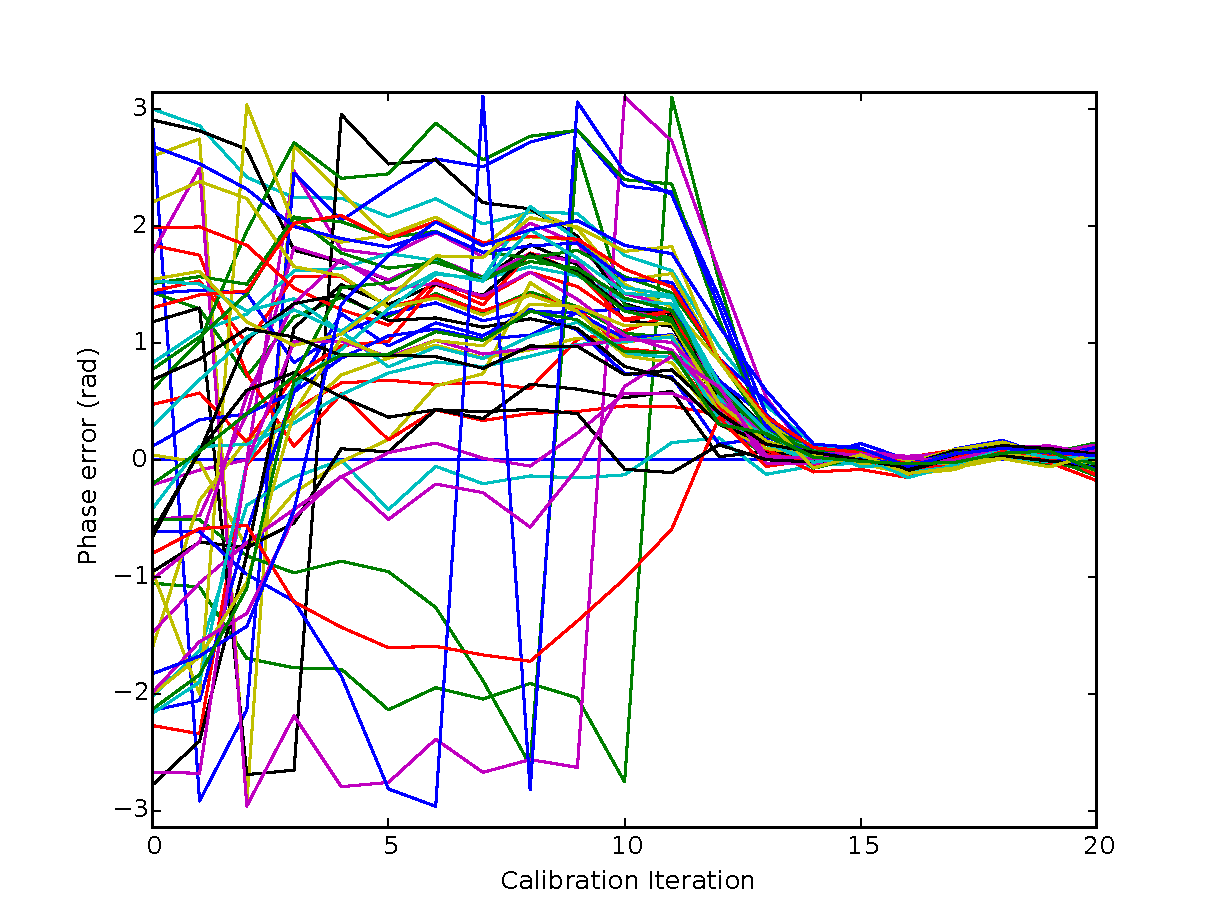
\includegraphics[width=\columnwidth]{figures/cal_paper_sim_phase.pdf}
\caption{Phase error of gain estimates as a function of iteration for simulated calibration. The gains were initialized with random phases, but the calibration loop was able to recover the correct phases after about 15 iterations. Each line represents an antenna in our 51 MWA antenna sample.
}
\label{fig:sim_phase}
\end{center}
\end{figure}

The estimated gain amplitudes for the simulations are shown in figure~\ref{fig:sim_amp}. The quantity plotted is the magnitude of the estimated gains over the true gains, $\left|g^{(n)}_a/g^T_a\right|$, which places all antennas on the same scale. We can see the amplitudes converge toward their true values around the same time as the phases (iteration $\sim$15). At the beginning of calibration we can see the value of the damping factor. At $n=0$, a couple of gains are shown to have abnormally high amplitude estimates, notably one about 3.3 times its true value (red line). These unbalanced high estimates caused the entire set of gains to be under estimated at $n=1$, even with a damping factor of 0.35. By $n=5$ the unbalanced amplitudes have been damped out and the calibration continues. Without the damping factor, the oscillation seen in the first couple iterations would have been significantly larger and taken much longer to fade out.

\begin{figure}
\begin{center}
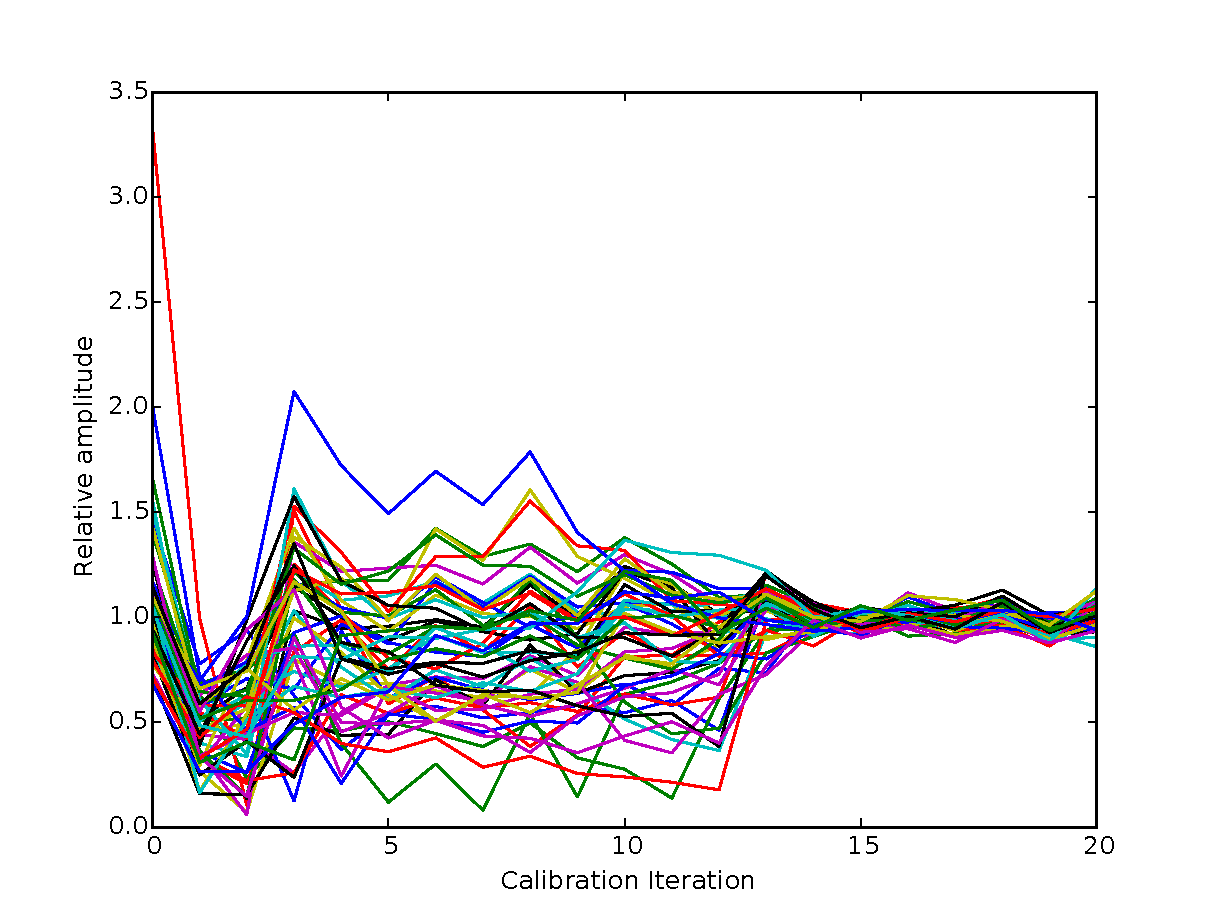
\includegraphics[width=\columnwidth]{figures/cal_paper_sim_amps.pdf}
\caption{Gain estimate amplitudes as a function of iteration for simulated calibration. Again, each line represents an antenna in the 51 MWA antenna sample. The gain estimates were initialized randomly, while the true values were unity. After about 15 iterations we see the calibration loop has settled around the correct values, with only noise remaining.}
\label{fig:sim_amp}
\end{center}
\end{figure}

Images created at the beginning of calibration and at the end are shown in figure~\ref{fig:sim_images}. Each image is 10~ms integration, corresponding to all snapshot images created with a given set of gain estimates. The top panel shows the image produced with our initialized unity gains. Because the phases are completely random, the image is essentially noise with the primary beam evident. After 20 iterations, the image is far more clear, shown in the bottom panel. Each of the ten simulated sources are clearly visible, indicated with red circles. 



\begin{figure}
\begin{center}
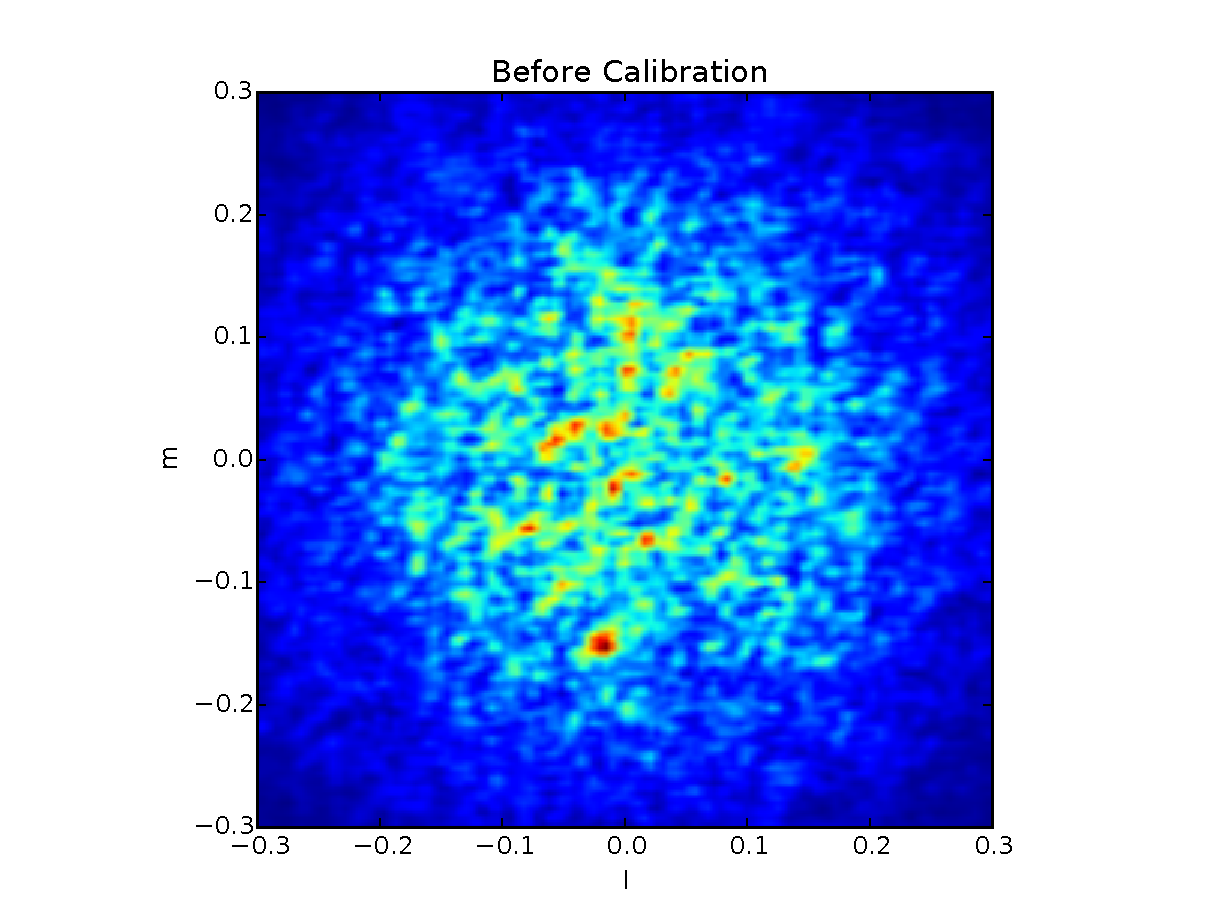
\includegraphics[width=\columnwidth]{figures/cal_paper_sim_image_before.pdf}
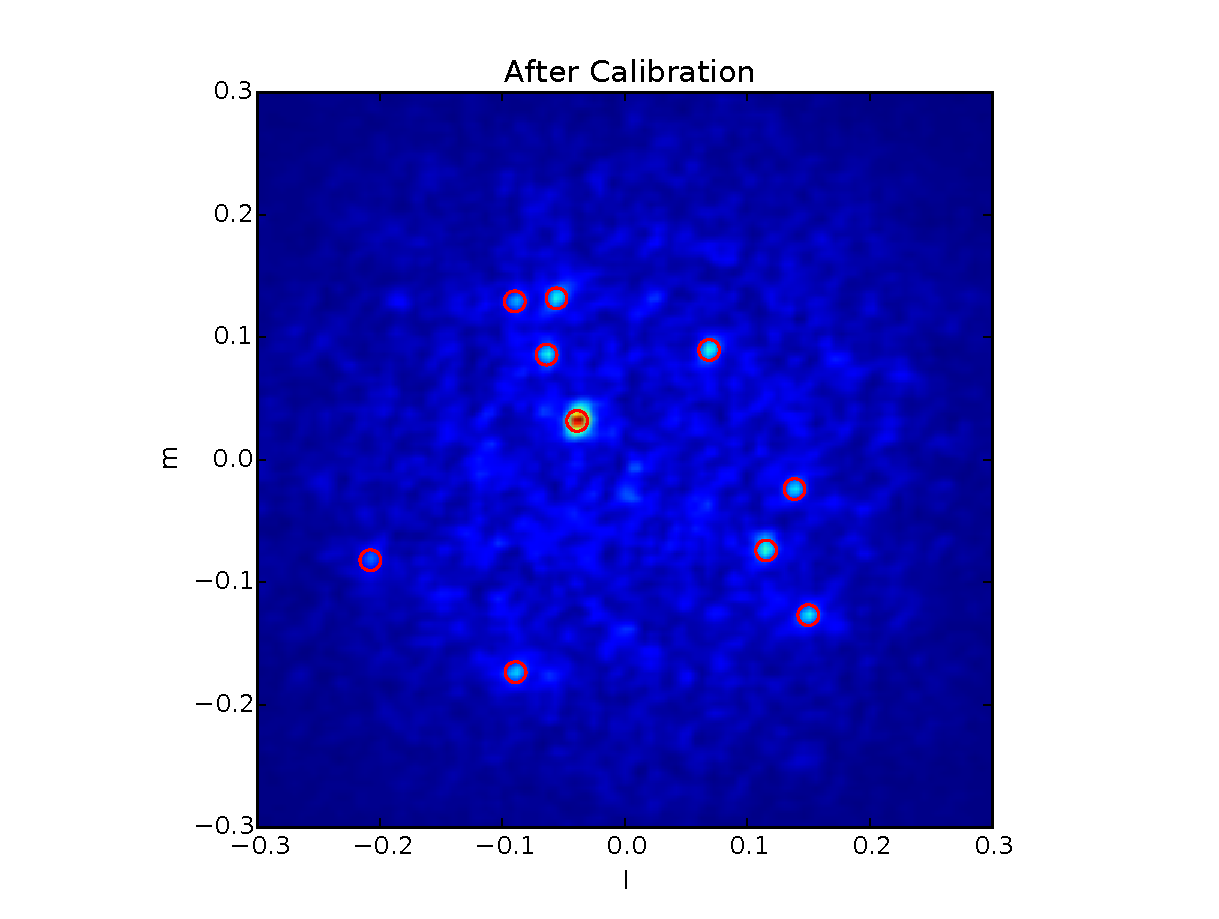
\includegraphics[width=\columnwidth]{figures/cal_paper_sim_image_after.pdf}
\caption{Images formed during simulated calibration. \emph{Top:} An image generated from a single frequency channel and 10 ms integration after the gain estimates are randomized. As expected with random phases, the image is completely noisy, with the shape of the primary beam evident. \emph{Bottom:} An image formed after calibration, again with a single frequency channel and 10 ms integration. The ten simulated (and modeled) point sources are easily visible, and highlighted with red circles.
}
\label{fig:sim_images}
\end{center}
\end{figure}

\section{Application to LWA data}\label{sec:data}
We next demonstrate our calibration algorithm using an observation from the LWA station in New Mexico. The data is from the LWA narrow-band transient buffer (TBN), with time ordered voltage data from 255 antennas within a core radius of 100~m. The central frequency is 74.03 MHz, and a bandwidth of 100 kHz and writeout timescale of 5.12 ms (frequency channel resolution of 195.3125 Hz). For this demonstration we limit ourselves to a single polarization.

After correcting for geometric cable delays, the instrument is naturally well calibrated, as was seen in the demonstration of the EPIC imager in \citealt{thy15c}. However, we will aim to improve yet on this calibration using our algorithm.

We proceed by forming model visibilities. We model only two bright objects as point sources: Cyg A with flux 16611.68 Jy \citep{coh07}; and Cas A with flux 17693.9 Jy \citep{kas07}. Because the raw data is attenuated by the primary beam of the instrument, we also account for this in our model using beam values consistent with \cite{hic12}.

We made several choices while studying the behavior of the LWA data to improve our calibration. We inspected the amplitudes of the voltages to be roughly consistent with average gain amplitudes of 0.25, so we initialized our gains at this level to allow the calibration to converge quickly. We also found a boost in signal to noise is achieved easily by averaging frequency channels and assuming the gains are constant within a sub-band. Here we average solutions across 150 channels, or about 29 kHz. With a fractional bandwidth $B/f_0 = 3.9 \times 10^{-4}$, we felt safe assuming a smooth bandpass. Because there is still a fair amount of noise in the data, a damping factor of $\gamma = 0.7$ was adopted.

Finally, we found that seven antennas\footnote{LWA antenna IDs 48, 85, 124, 148, 203, 217, and 244 were flagged.} produced unstable gain solutions, and in fact corrupted the ensemble. We therefore flagged these antennas for our analysis, resulting in a total of 248 antennas to calibrate. In each calibration loop, we form our feedback correlations and update our gain estimates over 10 timestamps (51.2 ms). We iterate the loop 30 times for a total of 1.536 seconds. The results of this experiment are shown in figures~\ref{fig:data_phase}~--~\ref{fig:data_images}.

Figure~\ref{fig:data_phase} shows the phase of our gain estimates over our 30 calibration iterations, again with each colored line representing a different antenna. Given the quality of uncalibrated image demonstrated in \cite{thy15c}, it is a bit surprising to see the phase variation in our solutions. However, the phases are relatively flat after about 15 iterations (modulo noise), and exhibit a central ``trunk" where the majority of phases are congregated. This behavior is suggestive that while the uncalibrated voltages were able to produce a viable image, the minor changes from our solutions will focus the image and improve the quality. The actual location of the ``trunk" (slightly negative) is simply determined by the reference antenna chosen to have identically zero phase, but happens to be slightly more positive than the bulk of antennas. We also note that some phases appear to exceed $\pm \pi$ radians, this is due to the unwrapping done for plotting clarity.

\begin{figure}
\begin{center}
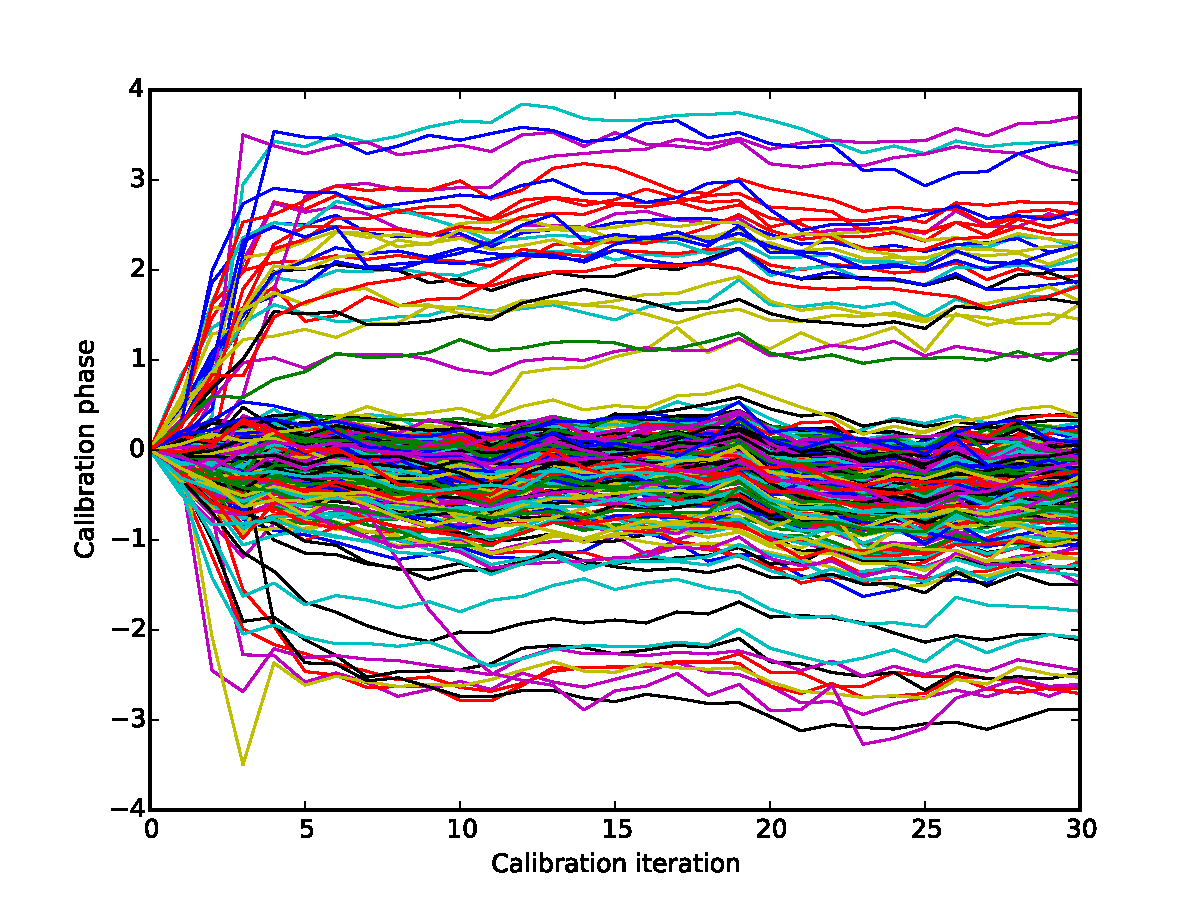
\includegraphics[width=\columnwidth]{figures/cal_paper_data_phases.pdf}
\caption{Gain phase solutions as a function of calibration iteration for an LWA TBN observation. The gain estimates are initialized with zero phase, but quickly span a $2\pi$ range, and settle into relatively flat, albeit noisy, solutions. The majority of phases congregate near zero, which is not surprising given the fairly good quality image produced from uncalibrated data.
}
\label{fig:data_phase}
\end{center}
\end{figure}

The gain amplitudes as a function of calibration iteration are shown in figure~\ref{fig:data_amp}. There is a fairly wide range in gain amplitudes (from 0.12 to 0.59). However, this is not surprising due to the non-uniformity in the cables from the antennas to the receivers. Again, the amplitudes are noisy by relatively flat.

\begin{figure}
\begin{center}
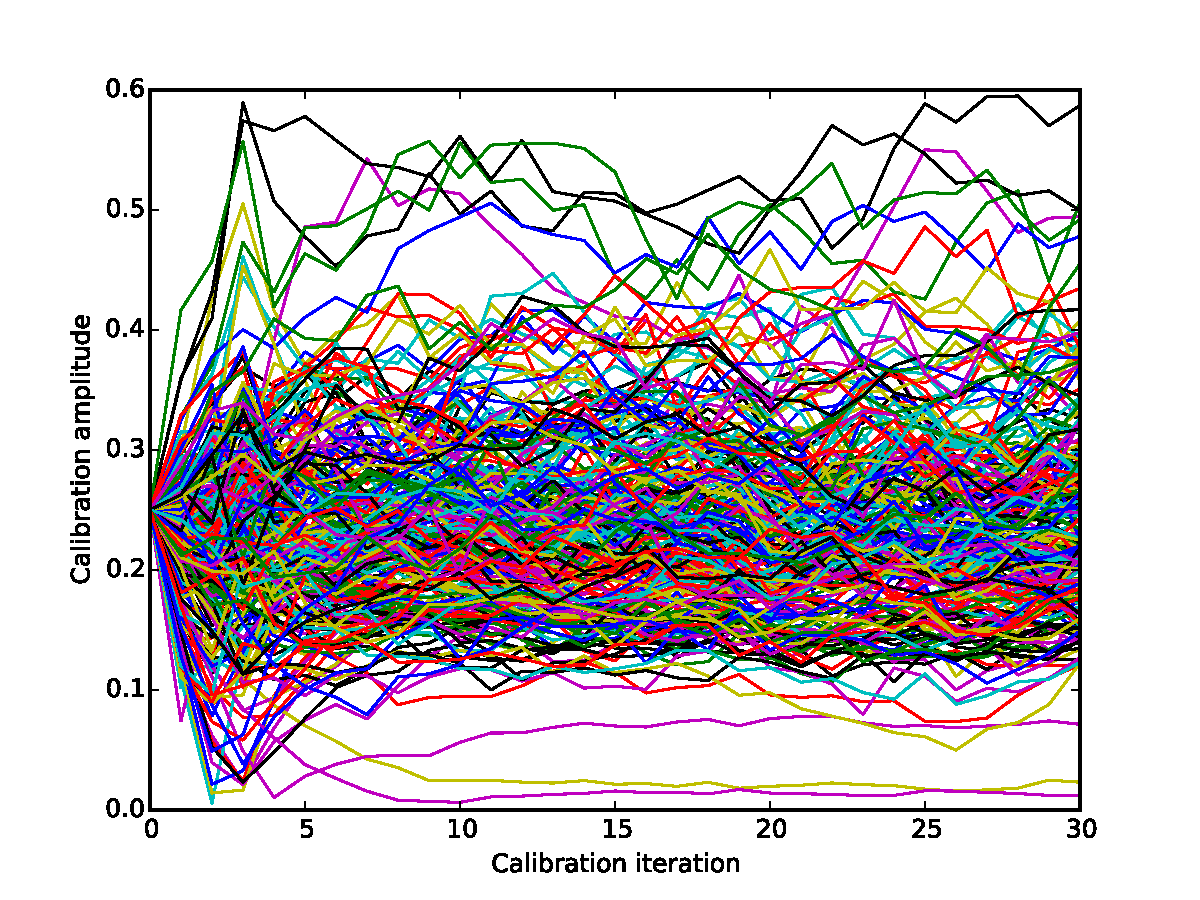
\includegraphics[width=\columnwidth]{figures/cal_paper_data_amps.pdf}
\caption{Gain amplitudes as a function of calibration iteration for an LWA TBN observation. The gains estimates were initialized with amplitude 0.25 after inspection of the electric field values compared to our model sky. The solutions are noisy, but flat. The range in amplitudes is due to the non-uniformity of cables between the LWA antennas and receivers.
}
\label{fig:data_amp}
\end{center}
\end{figure}

Figure~\ref{fig:data_images} shows the improvement in the images due to our calibration. The left panel shows the uncalibrated image integrated over 51.2 ms, 29 kHz. Cyg~A is prominent near the center of the image, and Cas~A is also clearly visible in the upper right. The middle panel shows the image produced after calibration with identical integration time and bandwidth. The sidelobes throughout the image are significantly suppressed, and the galactic plane is much more evident. We also note that the feature just to the right of Cyg~A is dimmer in the calibrated image, better matching the expected flux from the global sky model (GSM, \citealt{deo08}). We show the GSM modulated by two factors of the LWA primary beam in the right panel of figure~\ref{fig:data_images} for reference.

\begin{figure*}
\begin{center}
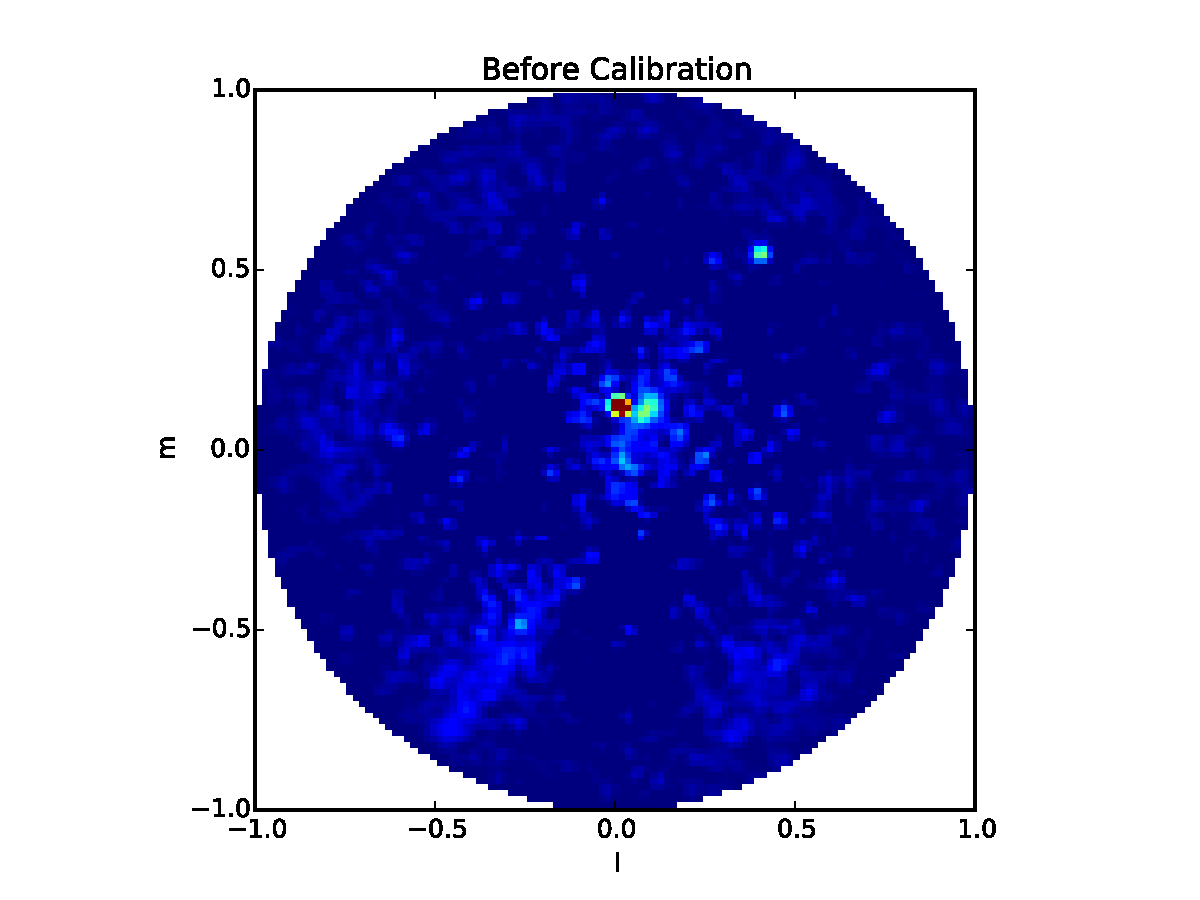
\includegraphics[width=0.33\linewidth]{figures/cal_paper_data_image_before.pdf}
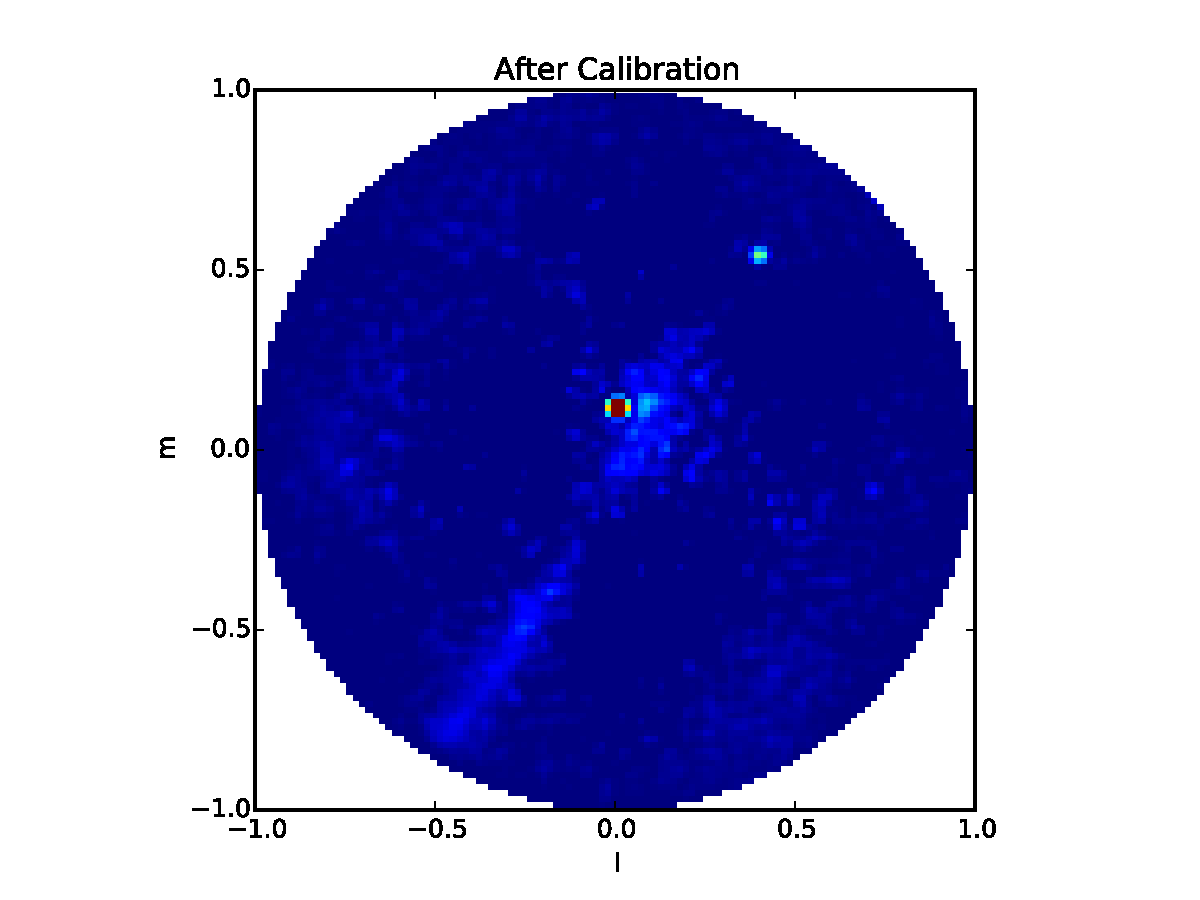
\includegraphics[width=0.33\linewidth]{figures/cal_paper_data_image_after.pdf}
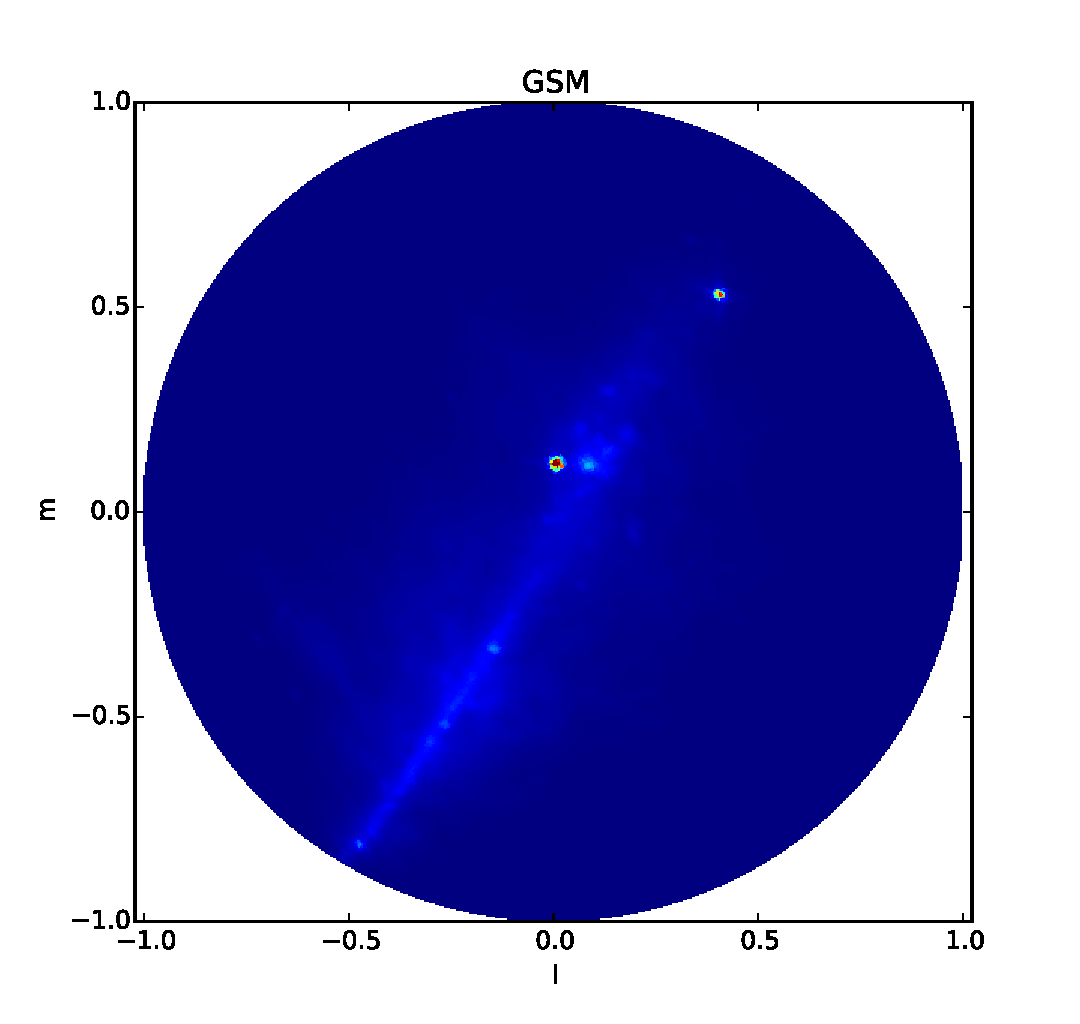
\includegraphics[width=0.33\linewidth]{figures/cal_paper_gsm_beam_weighted.pdf}
\caption{Images produced before (left) and after (middle) calibrating LWA data. These images were produces with 29 kHz bandwidth and 51.2 ms integration. The calibrated image shows significant reduction in sidelobe rumble throughout, while retaining the prominent Cyg~A and Cas~A sources. The galactic plane is also substantially more evident after calibration. For reference, the GSM is shown in the same coordinates and weighted by two factors of the LWA primary beam in the right panel.
}
\label{fig:data_images}
\end{center}
\end{figure*}

To compare the image qualities quantitatively we compute the dynamic range, defined as the peak of the image over the noise level. We estimate the noise level as the median of the absolute deviation of the image. With this metric we find the calibrated image to have a 55\% dynamic range improvement over the uncalibrated image.

\section{Noise analysis}\label{sec:noise}

Here we study the properties of our calibration solutions with respect to noise in the system. In order to compare to solutions from visibility-based calibration, we first derive the theoretical lower bound of the error in these solutions, given a set of measured visibilities, $\mathbf{V}$. We will do this through the Fischer information formalism and employ the Cram\'er-Rao lower bound 

Assume we did form visibilities with some integration time. Assuming the noise on each visibility, $\sigma_{ab}$, is independent, we can write the likelihood function of measuring $V_{ab}$ given the true value, the gains, and the noise.
\begin{equation}
\mathcal{L}(V_{ab};\mathbf{g}) = \frac{1}{2\pi \sigma_{ab}^2}\exp\left[-\frac{\left|V_{ab} - g_a g_b^* V_{ab}^T\right|^2}{2\sigma_{ab}^2}\right]
\end{equation}
Then the likelihood of the set of all visibilities is the product of all individual likelihoods.
\begin{equation}
\mathcal{L}(\mathbf{V};\mathbf{g}) = \prod_a \prod_{b > a} \mathcal{L}(V_{ab};\mathbf{g})
\end{equation}
The Fischer information matrix for the set of gain parameters is
\begin{equation}
\mathbf{F}^g_{ij} = \left<\left. \frac{\partial \ln \mathcal{L}(\mathbf{V};\mathbf{g})}{\partial g_i} \frac{\partial \ln \mathcal{L}(\mathbf{V};\mathbf{g})}{\partial g_j}\right|_\mathbf{g}\right>,
\end{equation}
where the expectation is taken over all possible visibility measurements.
We next evaluate the derivate of the log-likelihood.
\begin{equation}
\frac{\partial \ln \mathcal{L}(\mathbf{V};\mathbf{g})}{\partial g_i} = 
\sum_{a \ne i} \frac{g_a^* V_{ai}^{T*} (V_{ai} - g_a g_i^* V_{ai}^T)}{2 \sigma_{ai}^2}
\end{equation}

In order to find the Cram\'er-Rao lower bound on the variance of the complex parameter, $g_i$, we consider the term of the Fischer matrix where the first derivative is taken with respect to $g_i$, and the second with $g_i^*$. The result is
\begin{align}
\mathbf{F}^g_{ii} = & \left<\left[ \sum_{a \ne i} \frac{g_a^* V_{ai}^{T*} (V_{ai} - g_a g_i^* V_{ai}^T)}{2 \sigma_{ai}^2} \right] \right. \times \nonumber \\
& \left. \left[ \sum_{b \ne i} \frac{g_b V_{bi}^{T} (V_{bi}^* - g_b^* g_i V_{bi}^{T*})}{2 \sigma_{bi}^2} \right] \right> \nonumber \\
= &\sum_{a\ne i} \sum_{b \ne i} \frac{g_a^* g_b V_{ai}^{T*} V_{bi}^T}{4 \sigma_{ai}^2 \sigma_{bi}^2} \left< V_{ai}V_{bi}^* - g_i g_b^* V_{ai}V_{bi}^{T*}\nonumber \right.\\
&\left. - g_a g_i^* V_{ai}^T V_{bi}^* + g_a g_b^* |g_i|^2 V_{ai}^T V_{bi}^{T*}\right>
\label{eq:Fischer_before_expect}
\end{align}

The expected values are easy to evaluate. Each visibility will average to the ``true" value times the respective gains. The term with two visibilities will include a noise bias on autocorrelation terms.
\begin{equation}
\left<V_{ai}V_{bi}^*\right> = |g_i|^2 g_a g_b^* V_{ai}^T V_{bi}^{T*} + \sigma_{ai}^2 \delta_{ab}
\end{equation}
Here $\delta_{ab}$ is the Kronecker delta selecting the term where $a=b$ and the noise correlates. Plugging in the expectation values, equation \ref{eq:Fischer_before_expect} simplifies greatly to
\begin{equation}
\mathbf{F}^g_{ii} = \sum_{a \ne i} \frac{\left|g_a V_{ia}^T \right|^2}{4\sigma_{ai}^2}
\end{equation}

Finally we relate our result to the theoretical best uncertainty we can place on our unknown gain parameter using the Cram\'er-Rao lower bound.
\begin{equation}\label{eq:cramer_rao}
\sigma_{g_i}^2 \ge \left[ \mathbf{F}^g_{ii} \right]^{-1} = \left[ \sum_{a \ne i} \frac{\left|g_a V_{ia}^T \right|^2}{4\sigma_{ai}^2} \right]^{-1}
\end{equation}

We next run a set of EPICal simulations to compare the noisy results to the theoretical lower bound given a set of equivalent visibilities. Each simulation is run with a simple sky of a single point source with flux 1 Jy. We add noise to the system by adding a Gaussian-random complex value to each channelized electric field antenna measurement as in equation~\ref{eq:apply_gain}. The ``true" gains in our simulation are unity, as well as our initial estimate. This emulates a system where the initially volatile gain correction has been suppressed and only noise remains to corrupt our estimation, allowing us to run many simulations on a shorter timescale.

We vary two parameters in our simulations: the amount of noise added to our measurements, and the length of integration in each calibration loop. 

\section{Discussion}\label{sec:discussion}

\section*{Acknowledgements}
This work has been supported by the National Science Foundation through award AST-1206552.


%%%%%%%%%%%%%%%%%%%% REFERENCES %%%%%%%%%%%%%%%%%%

% The best way to enter references is to use BibTeX:

\bibliographystyle{../mnras}
\bibliography{../epic} % if your bibtex file is called example.bib



%%%%%%%%%%%%%%%%% APPENDICES %%%%%%%%%%%%%%%%%%%%%

%\appendix

%\section{Some extra material}

%If you want to present additional material which would interrupt the flow of the main paper,
%it can be placed in an Appendix which appears after the list of references.

%%%%%%%%%%%%%%%%%%%%%%%%%%%%%%%%%%%%%%%%%%%%%%%%%%


% Don't change these lines
\bsp	% typesetting comment
\label{lastpage}
\end{document}

% End of mnras_template.tex

%%%%%%%%%%%%%%%%% APPENDICES %%%%%%%%%%%%%%%%%%%%%

\appendix

\section{Software Architecture}\label{sec:software-modules}

EPIC is built using object oriented programming in Python and is built on
carefully crafted modules which closely represent real-life entities in radio 
interferometer arrays and observations. The essential modules along with their
key attributes and methods are illustrated in Fig.~\ref{fig:software-modules}.
These modules are described below.

\begin{figure*}
  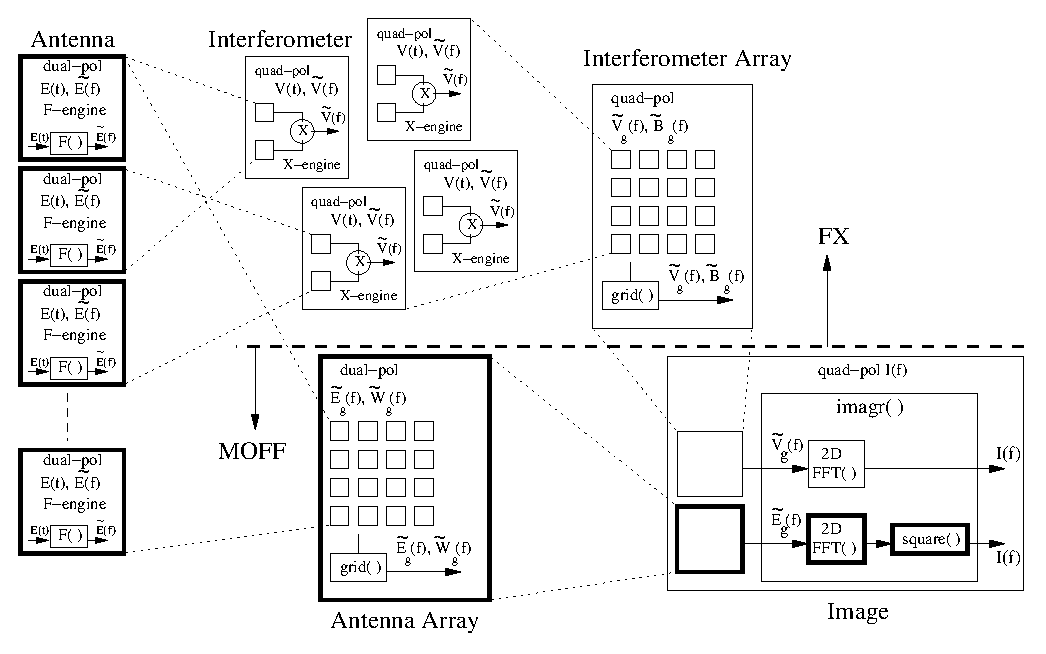
\includegraphics[width=\linewidth]{figureA1}
  % 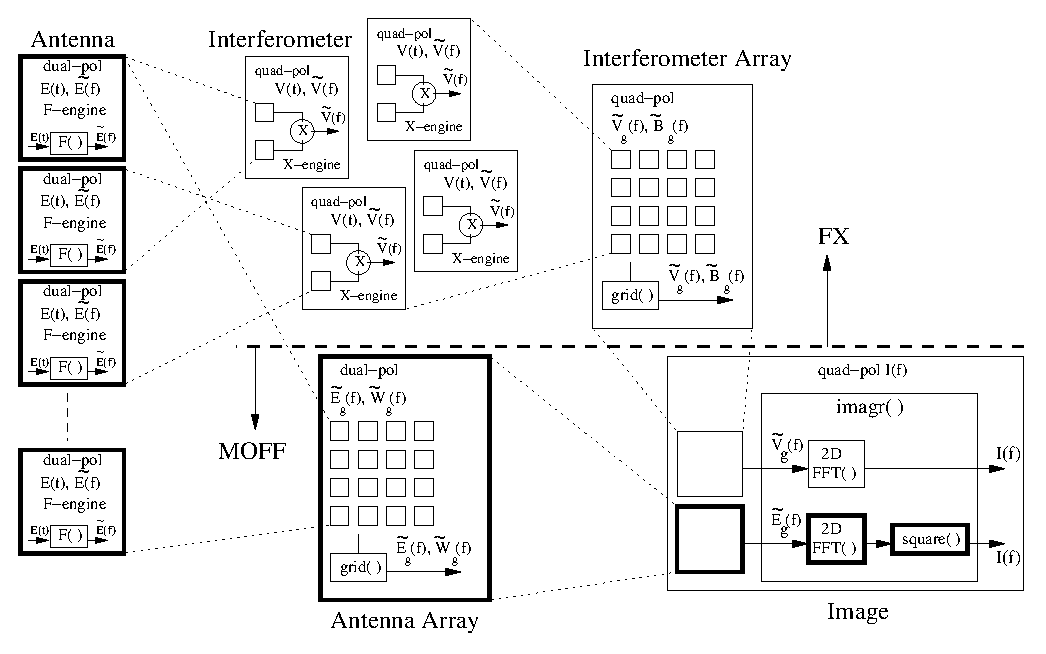
\includegraphics[width=\linewidth]{EPIC-modules}
  % 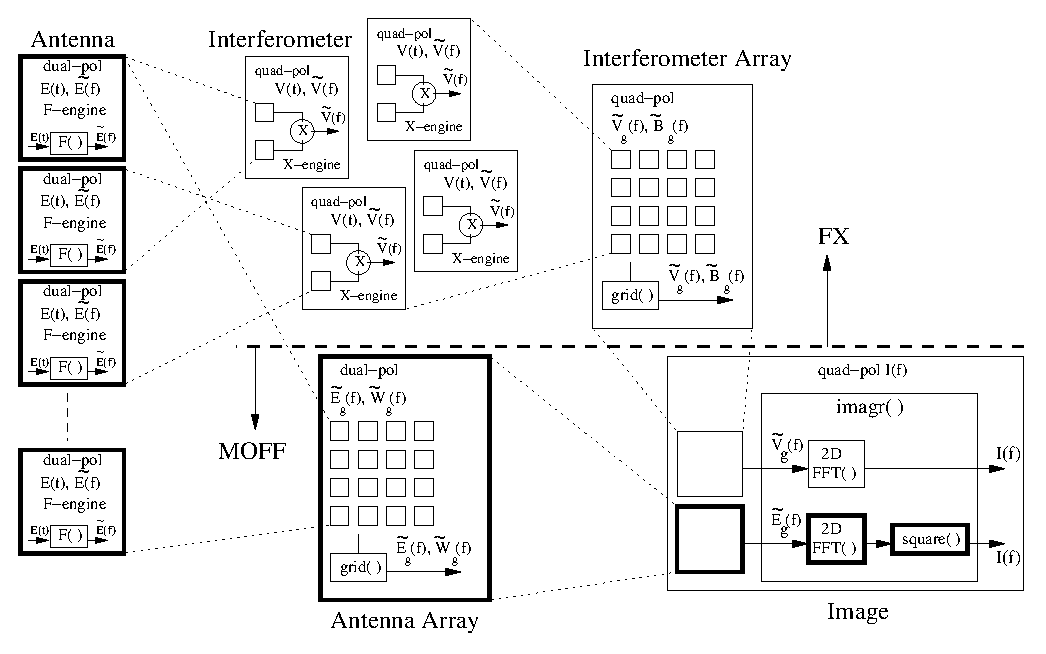
\includegraphics[width=\linewidth]{EPIC-modules.eps}
  \caption{Software architecture of EPIC with core modules, their essential
    attributes and functions. The antenna module forms the fundamental building 
    block. It consists of electric field time-series and spectra and the 
    F-engine that performs a temporal FFT to obtain electric field spectra from 
    the time-series. The interferometer module is made of a pair of antenna 
    modules. Its main function is the X-engine (FX or XF) to produce visibility 
    spectra. The antenna array module is made of all individual antenna modules
    as its components and contains collective properties about the antenna 
    subsystems. Its core function is the creation of antenna-to-grid mapping, 
    gridded aperture weights and electric fields. The interferometer array 
    module is very similar in principle to the antenna array module except it 
    operates on cross-correlations and produces gridded visibilities. The image 
    module takes gridded electric fields or visibilities and performs a 
    two-dimensional spatial FFT (and squares the intermediate image in case 
    of the former) to produce output images. Broadly, the MOFF algorithm is 
    implemented by modules below the horizontal dashed line while the 
    visibility-based imaging uses modules above the line. The exact processing 
    pathway implementing the MOFF algorithm is shown in bolded modules.}
  \label{fig:software-modules}
\end{figure*}

\subsection{Antenna Module}

The antenna module is a fundamental building block upon which all the other modules are built. There is one antenna module per antenna each having attributes -- the propagated electric field time-series, $\widetilde{E}(t)$, and spectrum $E(f)$ for both polarizations. The most important function inside this module is the F-engine that Fourier transforms time-series electric field data into spectra. 

The other function (not shown in the figure) is to update the data as new data 
streams in. This can also be parallelized. Another important attribute consists 
of antenna flags (not shown in the figure) for each polarization appropriate 
for the data stream being held by the module. 

\subsection{Interferometer Module}

The interferometer module holds the attributes and functions pertaining to a pair of antennas and represents the cross-correlation information obtained from the pair. Its primary attributes are the two antenna modules. It also contains four cross-polarized visibility time-series (even for the FX correlator for diagnostic purposes) and spectra. 

The critical component of the interferometer module is the X-engine. This is essentially a software analog of hardware correlators of real telescope systems. The X-engine can be toggled between two states of operation, namely, the FX and XF modes. The FX mode obtains the electric field spectra, $E(f)$ from the individual antenna modules inside this module and multiplies the two to obtain visibility spectra, $V(f)$. On the other hand, the XF mode cross-correlates the electric field time-series from its Antenna modules to obtain the visibilities as a function of lags, $V_t(\tau)$, which is then Fourier transformed to obtain $V(f)$. Both modules can operate on dual-polarizations to obtain all four cross-polarizations.

The other attributes (not shown in the figure) are the flags applicable for each
cross-polarization for the current data stream. Similar to the antenna module,
it has an update function that can update the visibilities $V_t(\tau)$ 
or $V(f)$ directly rather than through the electric fields of its 
component antennas. This functionality is to allow EPIC to operate while 
attached to the backend of traditional correlator systems. This feature is not 
utilized for purposes of this paper.

This module forms the fundamental unit for the interferometer array module 
(to be discussed below) and in general for visibility-based correlator and 
imaging systems. 

\subsection{Antenna Array Module}

The antenna array module consists of all the antenna modules as its attributes
and represents the collective properties of its component antennas. By virtue of 
holding each antenna data independently in their respective modules, the F-engine 
for the entire array can be distributed to the F-engines of the component 
antenna modules thus achieving a highly parallelized F-engine while emulating 
real telescope systems.

The primary attributes held by this module are the antenna aperture 
illumination weights and electric fields projected on the grid using the 
gridding convolution method described above and implemented by the gridding 
function in this module. Significant parts of the antenna-to-grid mapping and 
gridding convolution are parallelizable across antennas and frequencies.

Individual antenna flags are carried over as additional weights to be applied
to the gridded aperture illumination and electric fields. A series of data 
streams can be stacked up to take advantage of the array optimization available 
in Python. This module is also equipped to manage dual-polarization. 

\subsection{Interferometer Array Module}

Similar to the antenna array module, the interferometer array module consists of
individual interferometer modules. It can parallelize the correlator operations
by distributing the X-operation over the X-engines of its component 
interferometer modules. The interferometer-to-grid mapping and gridding 
convolution are very similar in nature to that of the antenna array module. 
Flag-based grid weights, stacking and ability to handle all four 
cross-polarizations are built into this module. 

\subsection{Image Module}

The image module is built as a general purpose module that can switch between 
operating on gridded electric fields or visibilities. At its heart, it consists
of a two-dimensional spatial FFT where the padding can be specified by the user 
to control the resolution in the output images. In case of MOFF imaging, there 
is an additional step of squaring the holographic electric field images. 

Besides its core functions of spatial Fourier transform and squaring, it can 
stack, accumulate and average images, and optionally remove the antenna
auto-correlations centred around the zero-spacing pixel in the $uv$ plane. 
It also handles all four cross-polarization products. Currently, it supports 
writing data out in standard FITS format. 

% \section{Some extra material}

% If you want to present additional material which would interrupt the flow of the main paper,
% it can be placed in an Appendix which appears after the list of references.

%%%%%%%%%%%%%%%%%%%%%%%%%%%%%%%%%%%%%%%%%%%%%%%%%%


% Don't change these lines
\bsp	% typesetting comment
\label{lastpage}
\end{document}

% End of mnras_template.tex
